%! Author = J. Villing
%! Date = 24.07.21

% Preamble
\documentclass[final]{fhnwreport}
% Packages
\usepackage{amsmath}
\usepackage{lipsum}
\usepackage[german]{babel}
\usepackage[style=ieee,urldate=comp,backend=biber]{biblatex}
\usepackage{listings}
\usepackage{pdflscape}
\usepackage{xcolor}
\usepackage{dirtree}
\usepackage{textcomp}
\usepackage{tabularx}
\usepackage{blindtext}
\usepackage{import}
\addbibresource{main.bib}

% Custom JS Listing support
\definecolor{mygreen}{rgb}{0,0.6,0}
\definecolor{mygray}{rgb}{0.5,0.5,0.5}
\definecolor{mymauve}{rgb}{0.58,0,0.82}
%Customize a bit the look
\lstset{ %
    backgroundcolor=\color{white}, % choose the background color; you must add \usepackage{color} or \usepackage{xcolor}
    basicstyle=\footnotesize, % the size of the fonts that are used for the code
    breakatwhitespace=false, % sets if automatic breaks should only happen at whitespace
    breaklines=true, % sets automatic line breaking
    captionpos=b, % sets the caption-position to bottom
    commentstyle=\color{mygreen}, % comment style
    deletekeywords={...}, % if you want to delete keywords from the given language
    escapeinside={\%*}{*)}, % if you want to add LaTeX within your code
    extendedchars=true, % lets you use non-ASCII characters; for 8-bits encodings only, does not work with UTF-8
    frame=single, % adds a frame around the code
    keepspaces=true, % keeps spaces in text, useful for keeping indentation of code (possibly needs columns=flexible)
    keywordstyle=\color{blue}, % keyword style
% language=Octave, % the language of the code
    morekeywords={*,...}, % if you want to add more keywords to the set
    numbers=left, % where to put the line-numbers; possible values are (none, left, right)
    numbersep=5pt, % how far the line-numbers are from the code
    numberstyle=\tiny\color{mygray}, % the style that is used for the line-numbers
    rulecolor=\color{black}, % if not set, the frame-color may be changed on line-breaks within not-black text (e.g. comments (green here))
    showspaces=false, % show spaces everywhere adding particular underscores; it overrides 'showstringspaces'
    showstringspaces=false, % underline spaces within strings only
    showtabs=false, % show tabs within strings adding particular underscores
    stepnumber=1, % the step between two line-numbers. If it's 1, each line will be numbered
    stringstyle=\color{mymauve}, % string literal style
    tabsize=2, % sets default tabsize to 2 spaces
    title=\lstname % show the filename of files included with \lstinputlisting; also try caption instead of title
}
%END of listing package%

\definecolor{darkgray}{rgb}{.4,.4,.4}
\definecolor{purple}{rgb}{0.65, 0.12, 0.82}

%define Javascript language
\lstdefinelanguage{JavaScript}{
    keywords={typeof, new, true, false, catch, function, return, null, catch, switch, const, let, var, if, in, while, do, else, case, break},
    keywordstyle=\color{blue}\bfseries,
    ndkeywords={class, export, boolean, throw, implements, import, this},
    ndkeywordstyle=\color{darkgray}\bfseries,
    identifierstyle=\color{black},
    sensitive=false,
    comment=[l]{//},
    morecomment=[s]{/*}{*/},
    commentstyle=\color{purple}\ttfamily,
    stringstyle=\color{red}\ttfamily,
    morestring=[b]',
    morestring=[b]"
}

\lstset{
    language=JavaScript,
    extendedchars=true,
    basicstyle=\footnotesize\ttfamily,
    showstringspaces=false,
    showspaces=false,
    numbers=left,
    numberstyle=\footnotesize,
    numbersep=9pt,
    tabsize=2,
    breaklines=true,
    showtabs=false,
    captionpos=b
}



\title{Peer-to-Peer Kommunikation für Sprachübertragung in einem Praxisrufsystem}  %Project Title
\author{IP6 - Bachelor Thesis}                      %Document Type => Technical Report, ...

\begin{document}
    \maketitle

    \vspace*{\fill}

    \begin{center}
        \renewcommand\arraystretch{2}
        \begin{tabular}{l l}
            Studenten & Joshua Villing \\
            Fachbetreuer & Daniel Jossen\\
            Auftraggeber & Daniel Jossen\\
            Studiengang & Informatik\\
            Hochschule & Hochschule für Technik
        \end{tabular}
    \end{center}

    \clearpage


%%---ABSTRACT----------------------------------------------------------------------------
    \pagenumbering{Roman}
    \section*{Management Summary}

''Ärzte und Zahnärzte haben den Anspruch in Ihren Praxen ein Rufsystem einzusetzen.
Dieses Rufsystem ermöglicht, dass der behandelnde Arzt über einen Knopfdruck Hilfe anfordern oder Behandlungsmaterial bestellen kann.
Heute kommerziell erhältlichen Rufsysteme beruhen meistens auf proprietären Standards und veralteten Technologien.''\cite{aufgabenstellung}
Mit dem Projekt ''IP5 Cloudbasiertes Praxisrufsystem'' wurde ein modernes Rufsystem ''Praxisruf'' mit reduziertem Funktionsumfang umgesetzt.
Die Problemstellung für dieses Projekt besteht darin, das bestehende Praxisrufsystem zu erweitern und fehlende Funktionen zu ergänzen.

Das erweiterte Praxisrufsystem hat zwei Hauptfunktionen.
Es kann als Gegensprechanlage verwendet werden und bietet die Möglichkeit Benachrichtigungen in einer Praxis zu versenden.
Das Rufsystem wird von Endbenutzern über IPads bedient.
Die dazu entwickelte Applikation ermöglicht es, Sprachverbindungen zwischen zwei oder mehr Teilnehmern aufzubauen und Benachrichtigungen zu versenden.
Der Inhalt von empfangenen Benachrichtigungen kann bei entsprechender Konfiguration automatisch vorgelesen werden.
Welche Sprachverbindungen und Benachrichtigungen zur Verfügung stehen, wird von Administratoren über eine Weboberfläche konfiguriert.

Nach Projektabschluss stehen drei Optionen für das weitere Vorgehen offen:

\textbf{1. Produktiver Einsatz}

Mit den Erweiterungen, die in diesem Projekt umgesetzt wurden, erfüllt Praxisruf die Mindestanforderungen an ein modernes Praxisrufsystem.
Dementsprechend könnte das System bereits heute als produktives Rufsystem in einem Praxisumfeld eingesetzt werden.
Praxisruf allerdings noch nicht in einem produktiven Umfeld getestet.
Es muss verifiziert werden, dass das System mit der Last, die in einem produktiven Umfeld entsteht umgehen kann und den Qualitätsansprüchen von Praxismitarbeitenden entspricht.
Weiter hat das System noch Lücken in den Bereichen Benutzerfreundlichkeit und Konfigurierbarkeit.
Aufgrund dieser Einschränkung wird davon abgeraten, Praxisruf produktiv einzusetzen.

\textbf{2. Test in Pilotbetrieb}

Um Praxisruf in einem produktiven Umfeld zu testen, könnte es als Pilotprojekt in einzelnen Praxen eingesetzt werden.
In diesem Pilotprojekt könnten Rückmeldung von Praxismitarbeitenden gesammelt und Performancemetriken gemessen werden.
Aufgrund dieser Ergebnisse kann evaluiert werden, welche Erweiterungen an Praxisruf vorgenommen werden müssen.

\textbf{3. Weiterentwicklung für kommerzielle Nutzung}

Praxisruf ist heute darauf ausgelegt, in genau einer Praxis eingesetzt zu werden.
Um es als kommerziell erhältliches System anbieten zu können muss es um Mandantenfähigkeit erweitert werden.
Es muss möglich sein mehrere Systemkonfigurationen zu verwalten, wobei diese strikt voneinander getrennt bleiben.
Weiter wird empfohlen die Berechtigungsprüfung in Praxisruf zu erweitern und einen externen Identity-Provider anzubinden.

\textbf{Empfehlung}

Es wird empfohlen mit der Option zwei ''Test in Pilotbetrieb'' fortzufahren.
Durch Pilotbetrieb in einem realistischen Umfeld, kann garantiert werden, dass Praxisruf den Qualitätsanspruchen der Anwender enstpricht.
Weiter kann die Verwendung des Systems beobachtet werden und in hinsicht Performance und Benutzerfreundlichkeit wo nötig verbessert werden.
Sollte Praxisruf als kommerzielles System angeboten werden, wird zudem empfohlen die Option drei ''Weiterentwicklung für kommerzielle Nutzung'' zu verfolgen.
Die Erweiterung um Mandantenfähigkeit und Anbindung eines externen Identity-Providers sind für die kommerzielle Nutzung des Systems unerlässlich.

\clearpage



%%---TABLE OF CONTENTS-------------------------------------------------------------------
    \setcounter{tocdepth}{2}
    \tableofcontents
    \clearpage

%%---TEXT--------------------------------------------------------------------------------
    \pagenumbering{arabic}
    \section{Einleitung}

''Ärzte und Zahnärzte haben den Anspruch in Ihren Praxen ein Rufsystem einzusetzen.
Dieses Rufsystem ermöglicht, dass der behandelnde Arzt über einen Knopfdruck Hilfe anfordern oder Behandlungsmaterial bestellen kann.''\cite{aufgabenstellung}
Mit diesem Projekt wurde ein cloudbasiertes Praxisrufsystem konzipiert und umgesetzt.
Dazu wurde das im Vorgängerprojekt ''IP5 Cloudbasiertes Praxisrufsystem'' umgesetzte Praxisrufsystem erweitert.
Das erweiterte System ermöglicht es Benachrichtigungen zu versenden und Sprachverbindungen zwischen Teilnehmern aufzubauen.
Als Benutzeroberfläche dient dabei eine native iOS Applikation.
Folgende Abbildungen zeigen die Startseite der iOS Applikation (Abbildung 1.1) sowie die Ansicht während eines aktiven Gruppenanrufs (Abbildung 1.2).

\begin{figure}[h]
    \centering
    \begin{minipage}[b]{0.4\textwidth}
        \fbox{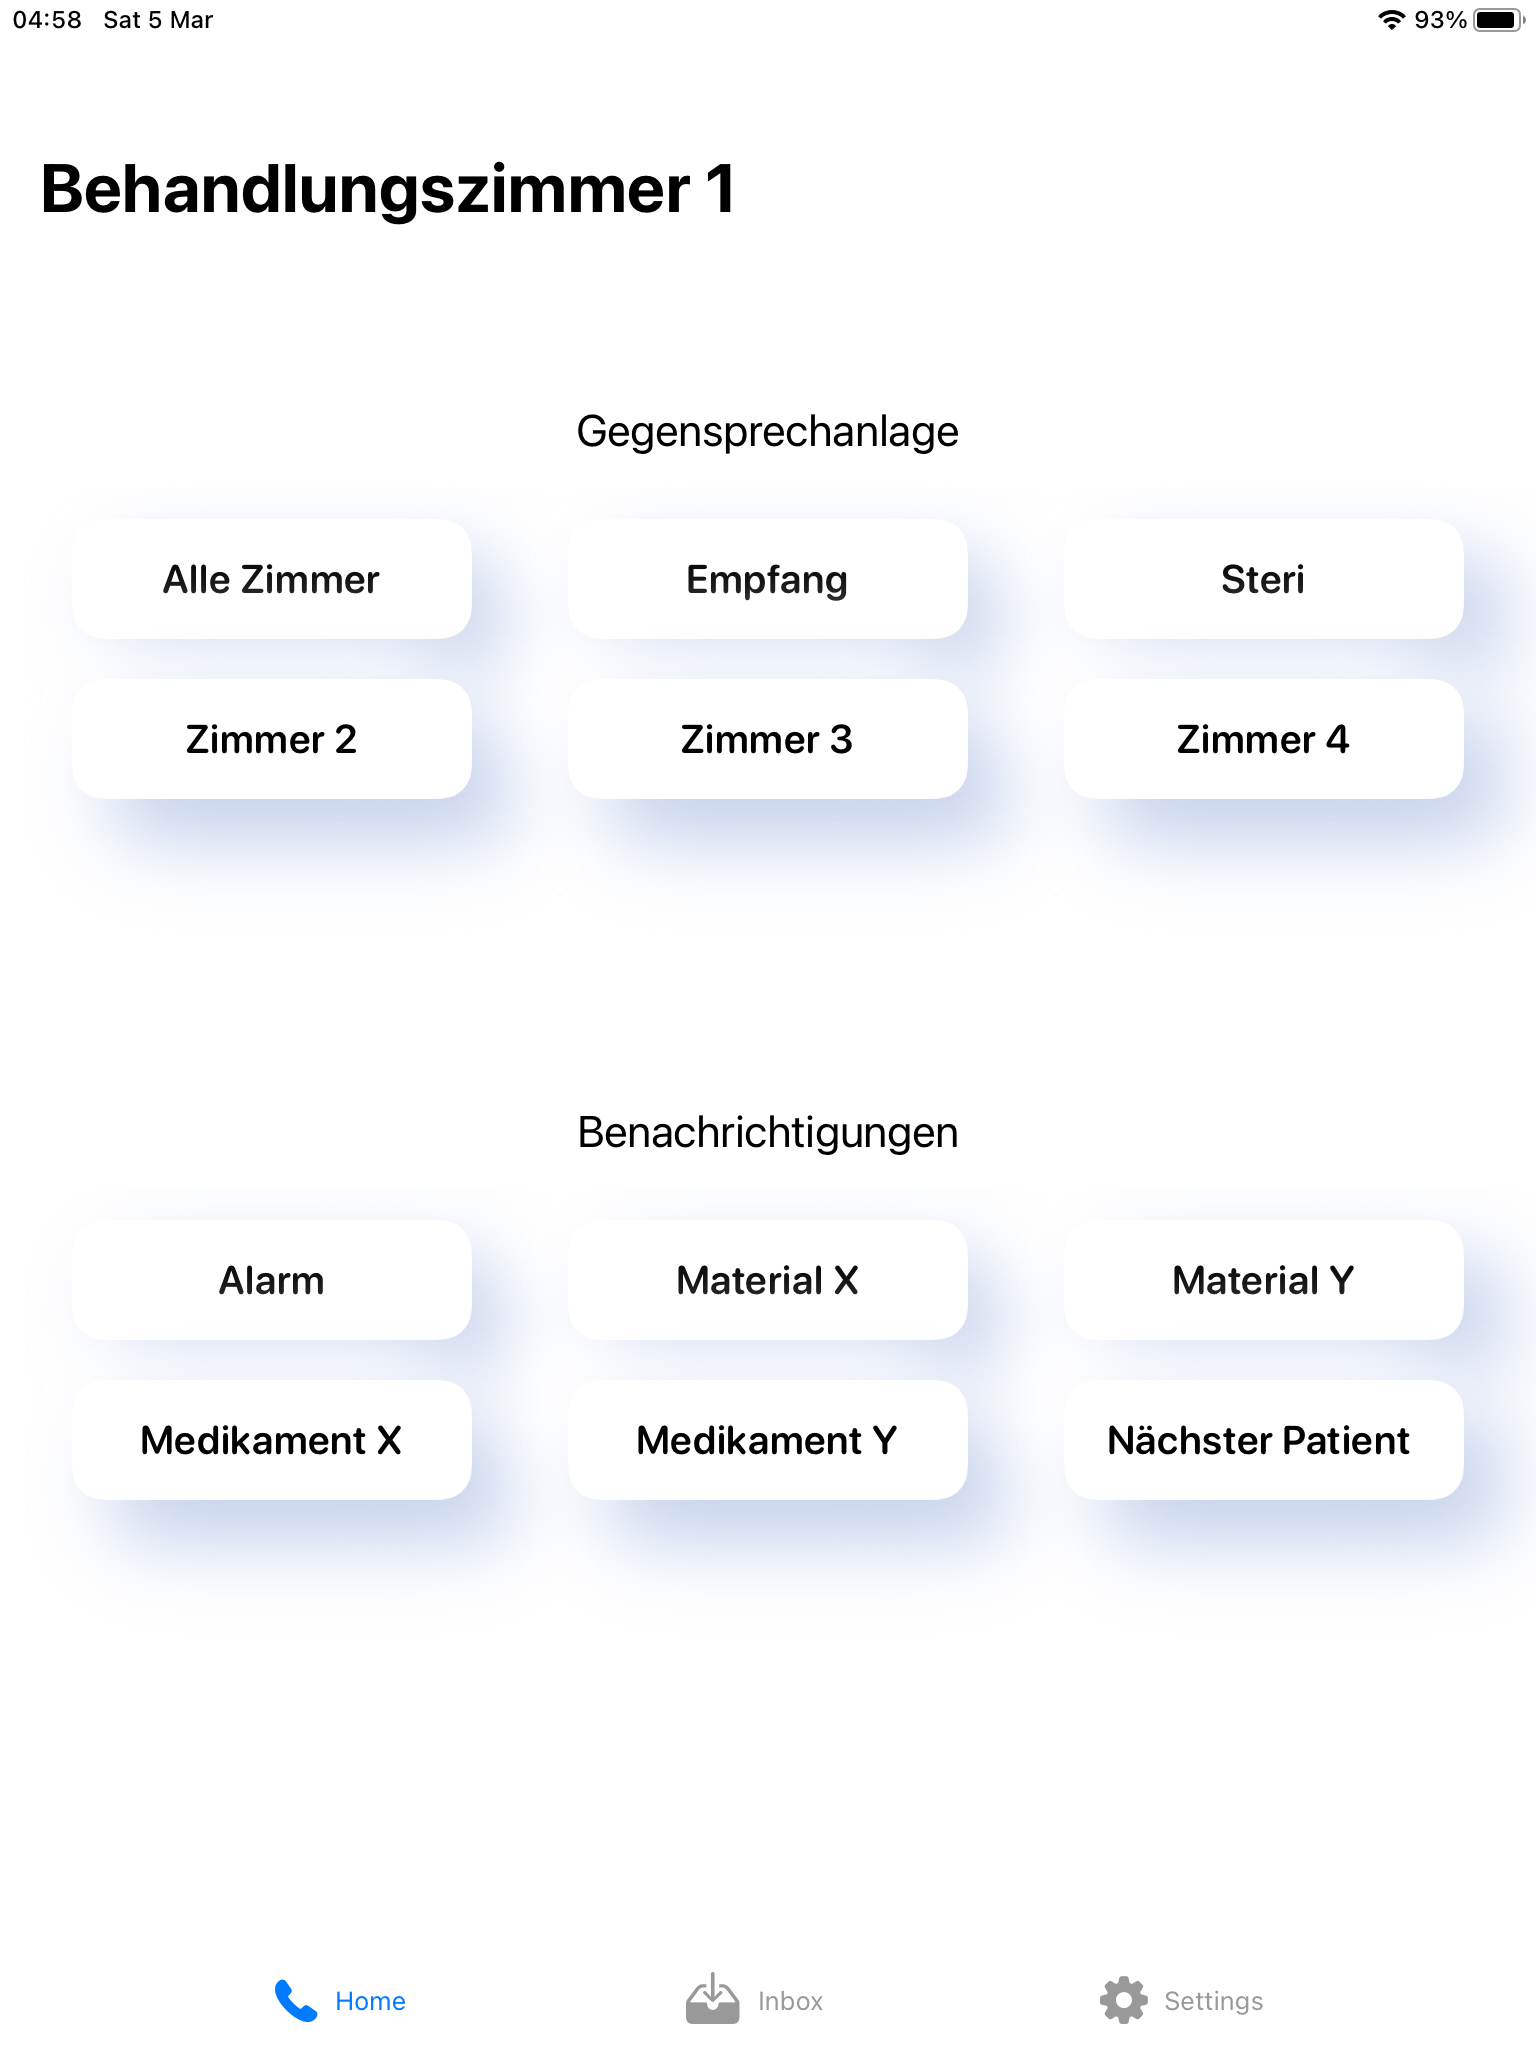
\includegraphics[width=\textwidth]{graphics/screenshots/app/home}}
        \caption{Praxisruf Startseite}
    \end{minipage}
    \hfill
    \begin{minipage}[b]{0.4\textwidth}
        \fbox{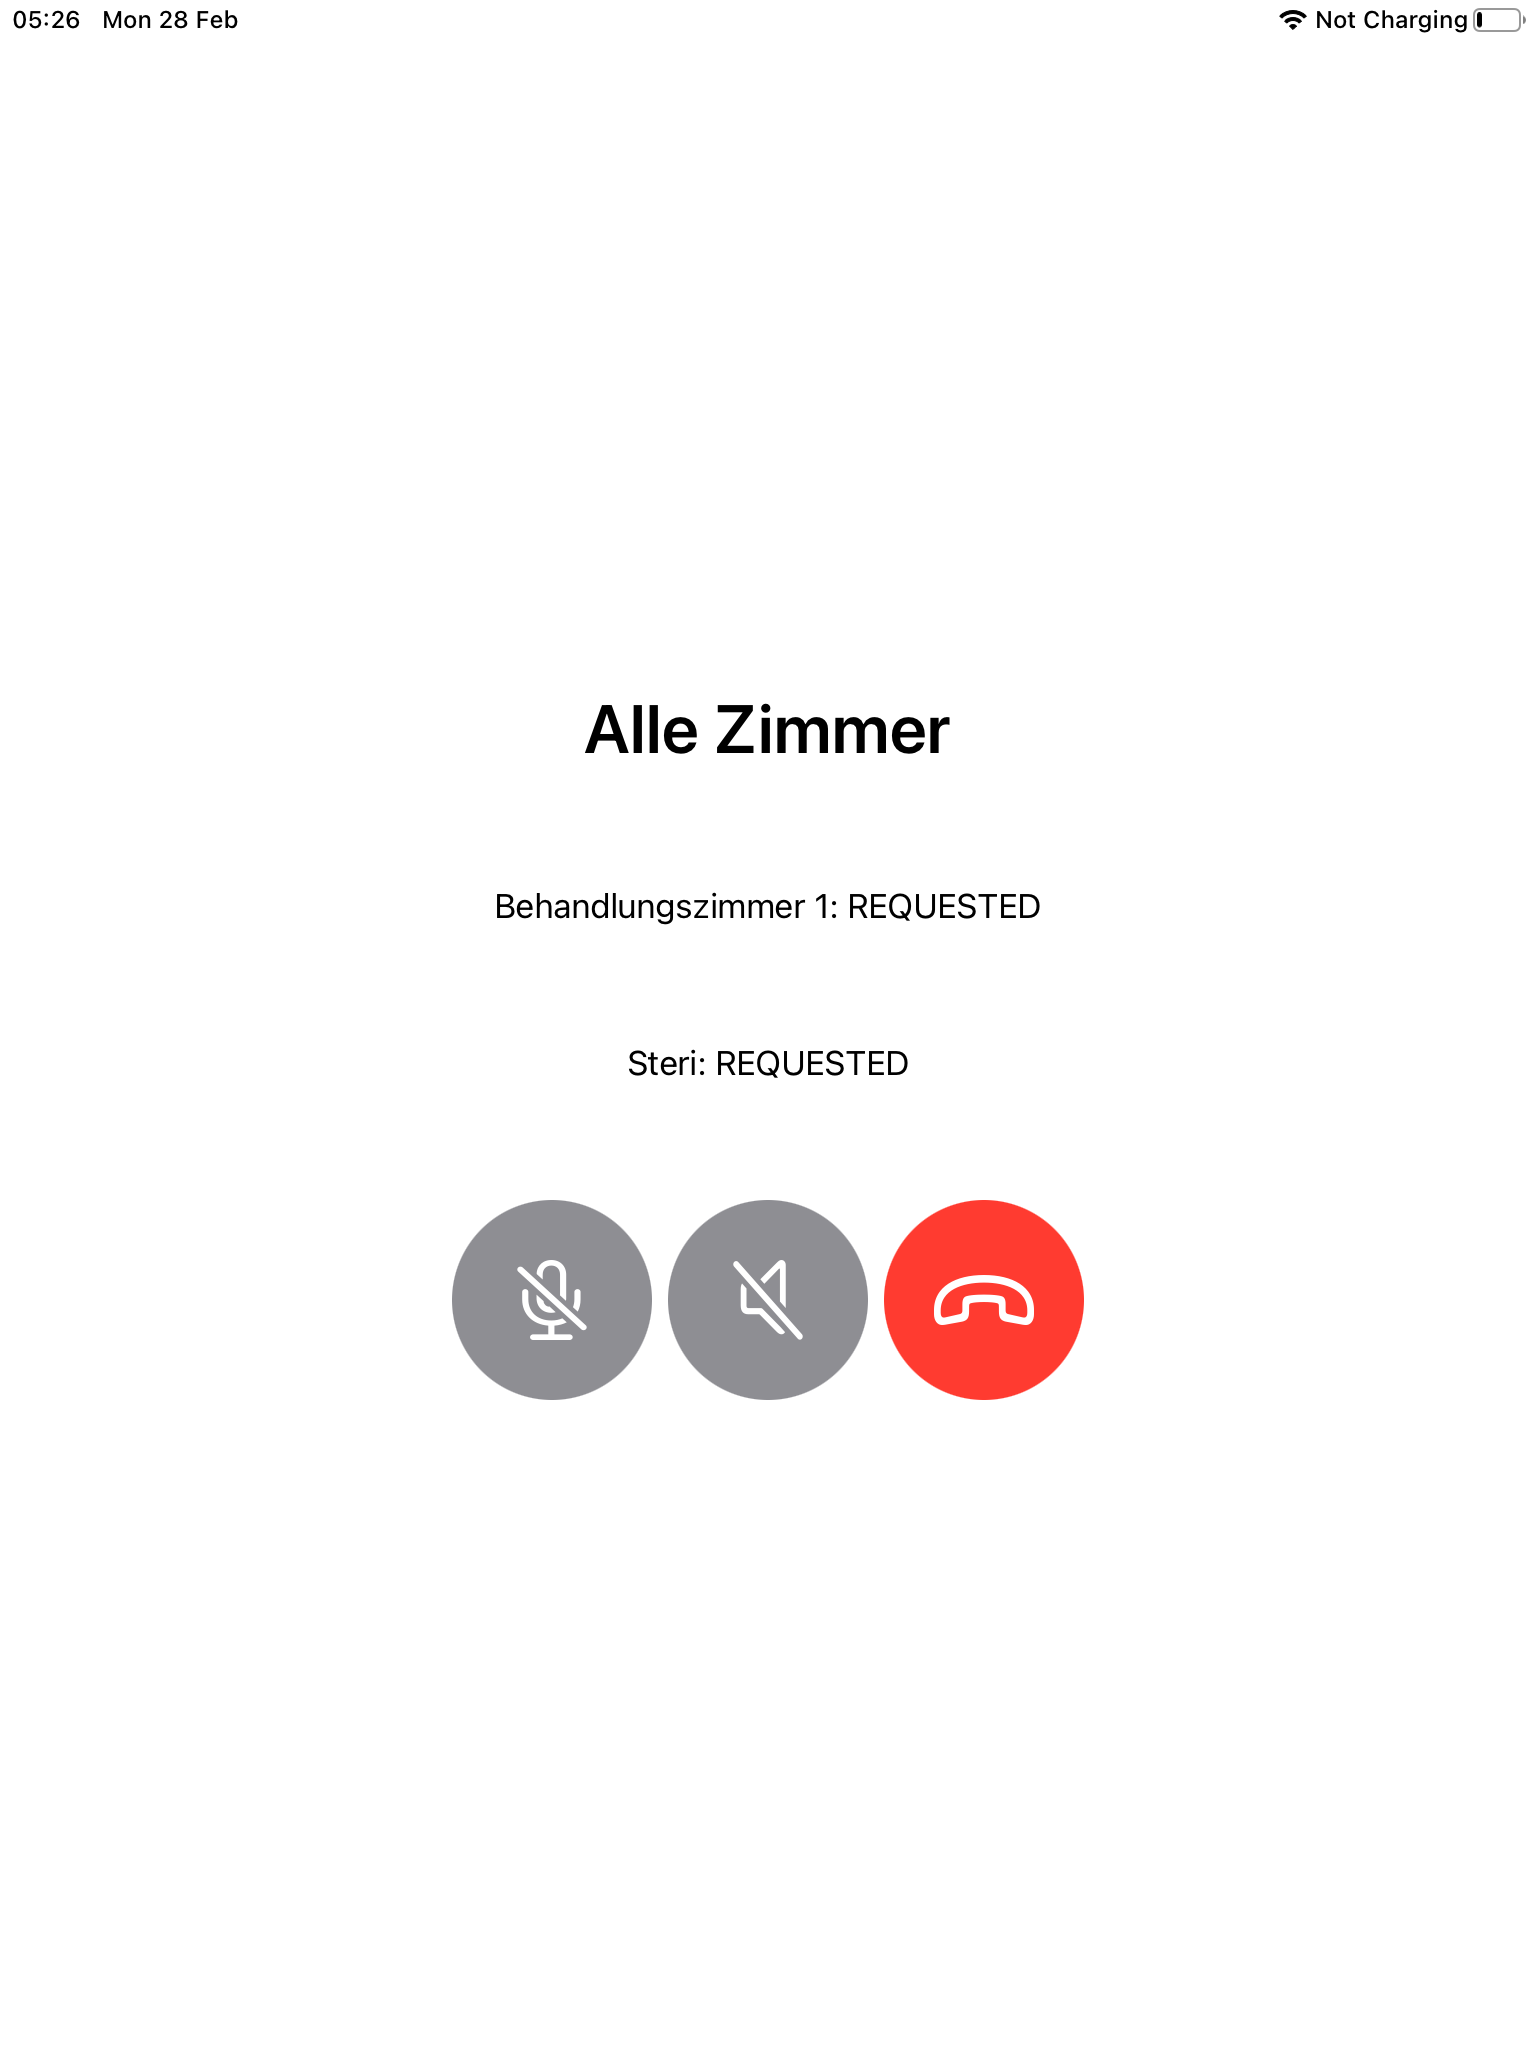
\includegraphics[width=\textwidth]{graphics/screenshots/app/call}}
        \caption{Aktiver Anruf}
    \end{minipage}
    \label{fig:MobileClient-ScreensIntroduction}
\end{figure}

Auf der Startseite der Applikation können per Knopfdruck Benachrichtigungen versendet und Sprachverbindungen gestartet werden.
Empfangene Benachrichtigungen werden als Push-Benachrichtigung angezeigt und in einer Inbox gesammelt.
Bei entsprechender Konfiguration wird zudem der Inhalt von empfangenen Benachrichtigungen automatisch vorgelesen.
Sprachverbindungen können zwischen zwei oder mehr Teilnehmern aufgebaut werden.
Das System unterstützt sowohl private Gespräche als 1:1 Verbindungen wie auch Gruppenunterhaltungen als 1:N Verbindungen.

Welche Buttons und damit welche Benachrichtigungen und Sprachverbindungen zur Verfügung stehen, wird durch Praxisadministratoren konfiguriert.
Die Konfiguration von Buttons für Sprachverbindungen beinhaltet, mit welchen Empfängern eine Verbindung aufgebaut wird.
Die Konfiguration von Buttons für Benachrichtigungen definiert den Inhalt der Benachrichtigung, welche Empfänger sie erhalten und ob die Benachrichtigung vorgelesen wird.
Für die Verwaltung dieser Konfiguration kann durch eine Weboberfläche vorgenommen werden.
Abbildung 1.3 zeigt die Übersicht verfügbarer Benachrichtigung in dieser Weboberfläche.

\begin{figure}[h]
    \centering
    \begin{minipage}[b]{1\textwidth}
        \fbox{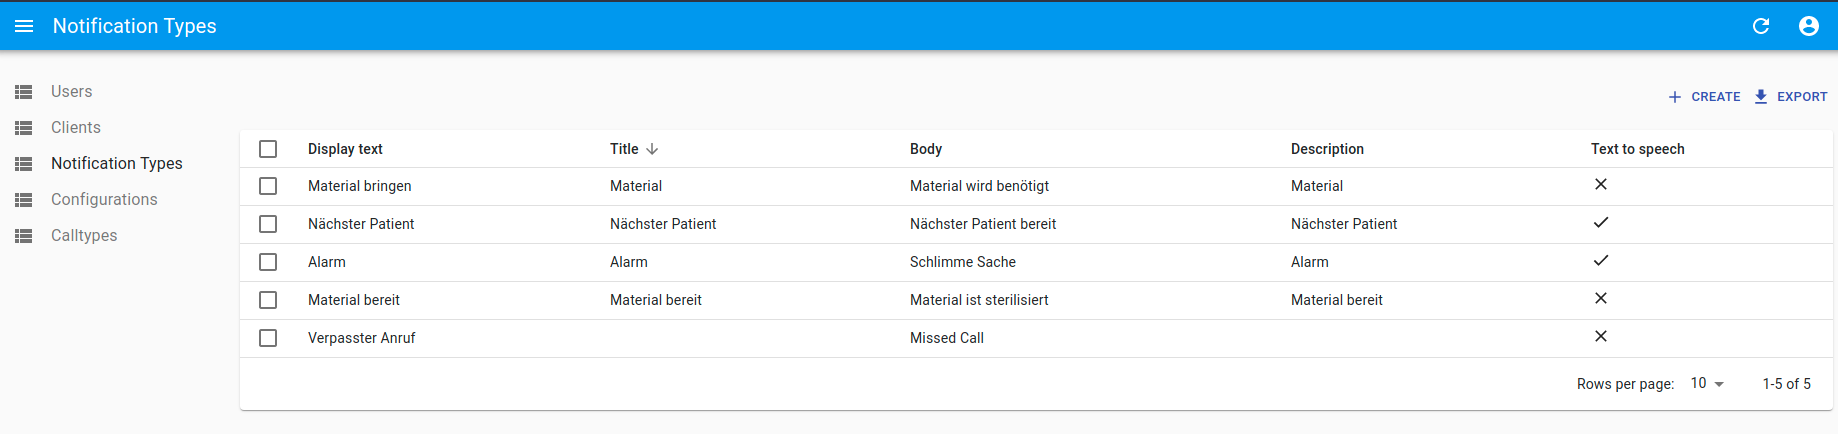
\includegraphics[width=\textwidth]{graphics/screenshots/admin_ui_notification_types}}
        \caption{Praxisruf Startseite}
    \end{minipage}
    \label{fig:AdminUI-Introduction}
\end{figure}

Die Grundlage für das entwickelte Praxisrufsystem wurde im Rahmen der Projektarbeit ''IP5 Cloudbasiertes Praxisrufsystem'' erarbeitet.
Im Rahmen des Vorgängerprojektes wurde bereits ein Praxisrufsystem mit eingeschränktem Funktionsunmfang entwickelt.
Die in diesem Projekt entwickelte Lösung ist eine Erweiterung des bestehenden Systems.
Das zuvor umgesetzte System unterstützt das Versenden und Empfangen von Benachrichtigungen.
Sprachsynthese für Benachrichtigungen und Sprachverbindungen für eine Gegensprechanlage konnten im Rahmen des Vorgängerprojektes nicht umgesetzt werden.
Die zentrale Aufgabenstellung für dieses Projekt war es, das System zu erweitern so, dass Benachrichtigungen vorgelesen und Sprachverbindungen aufgebaut werden können.
Die Bedienung des Praxisrufsystems soll weiterhin über eine mobile Applikation möglich sein.
Dazu soll eine neue, native iOS Applikation entwickelt werden.
Diese ersetzt die bestehende App und muss alle bestehenden Funktionen unterstützten.
Sie muss zudem Sprachverbindungen zu anderen Teilnehmern aufbauen und den Inhalt von Benachrichtigungen vorlesen können.

Wie in der Aufgabenstellung beschrieben, hat eine Marktanalyse im Vorfeld dieses Projektes gezeigt, dass bestehende kommerzielle Praxisrufsysteme veraltete Technologien einsetzten.
Diese Systeme sind aufwändig zu installieren und skalieren schlecht.
Sie können weiter nicht einfach in ein TCP/IP-Netzwerk eingebunden und über externe APIs angesteuert werden.\cite{aufgabenstellung}
Das im Rahmen des Vorgängerprojektes umgesetzte System löst diese Probleme bereits teilweise.
Mit dem Cloudservice bietet das System einen zentralen Dienst, welcher über eine Http Schnittstelle ansprechbar ist.
Diese ermöglicht die Verwaltung der Systemkonfiguration und stellt Benachrichtigung anhand der Konfiguration an relevante Empfänger zu.
Dadurch ist es einfacher möglich, das System in Netzwerke einzubinden, zu skalieren und neue Endgeräte anzubinden.
Das Vorgängersystem unterstützt aber noch nicht alle Funktionen, die ein Praxisrufsystem bieten muss.
Die meisten kommerziell erhältlichen Lösungen können als Gegensprechanlage verwendet werden\cite{aufgabenstellung}.
Ein vollständiges Praxisrufsystem muss deshalb unbedingt als Gegensprechanlage verwendet werden können.
Mit der Integration von Sprachsynthese für Benachrichtigungen kann sich das System weiter von bestehenden Lösungen absetzten.
Ein weiterer Schwachpunkt des Vorgängerprojektes ist die mobile Applikation.
Diese wurde mit einer geteilten Codebasis für iOS und Android entwickelt.
Im Fazit des Vorgängerprojekts wurde festgehalten, dass diese Applikation idealerweise neu als native Applikation entwickelt werden sollte.
Dadurch könne effizienter Betrieb, Wartung sowie Hardware- und Betriebssystemkomaptibilität langfristig gewährleistet werden.\cite{ip5}

Das umgesetzte System besteht aus drei Applikationen.
Der zentrale Cloudservice dient zur Verwaltung der Konfiguration und dem Vermitteln von Nachrichten zwischen Endgeräten.
Das Admin UI bietet eine Weboberfläche mit der die Konfiguration des Cloudservice verwaltet werden kann.
Mit dem Mobile Client bietet das System eine iOS App über welche Sprachverbindungen aufgebaut und Benachrichtigungen versendet werden können.
Für das Versenden von Benachrichtigungen, sendet ein Mobile Client eine HTTP Anfrage an den Cloudservice.
Der Cloudservice findet in der Konfiguration alle relevanten empfänger und leitet die Benachrichtigung an diese weiter.
Für die Zustellung von aus dem Cloudservice an Mobile Clients wird Firebase Cloud Messaging verwendet.

Für die Synthese von Sprachdaten wurde eine Anbindung an AWS Polly im Cloudservice implementiert.
Der Cloudservice bietet neue eine Http Schnittstelle, über welche Clients Sprachdaten für Benachrichtigungen beziehen können.
Durch diese Lösung müssen die Endgeräte die Anbindung an den Sprachsyntheseprovider nicht selbst implementierten.
Dies bietet den Vorteil das der Provider leicht ausgewechselt werden kann und dass die Anbindung von zukünftige Platformen übernommen werden kann.

\begin{figure}[h]
    \centering
    \begin{minipage}[b]{0.75\textwidth}
        \fbox{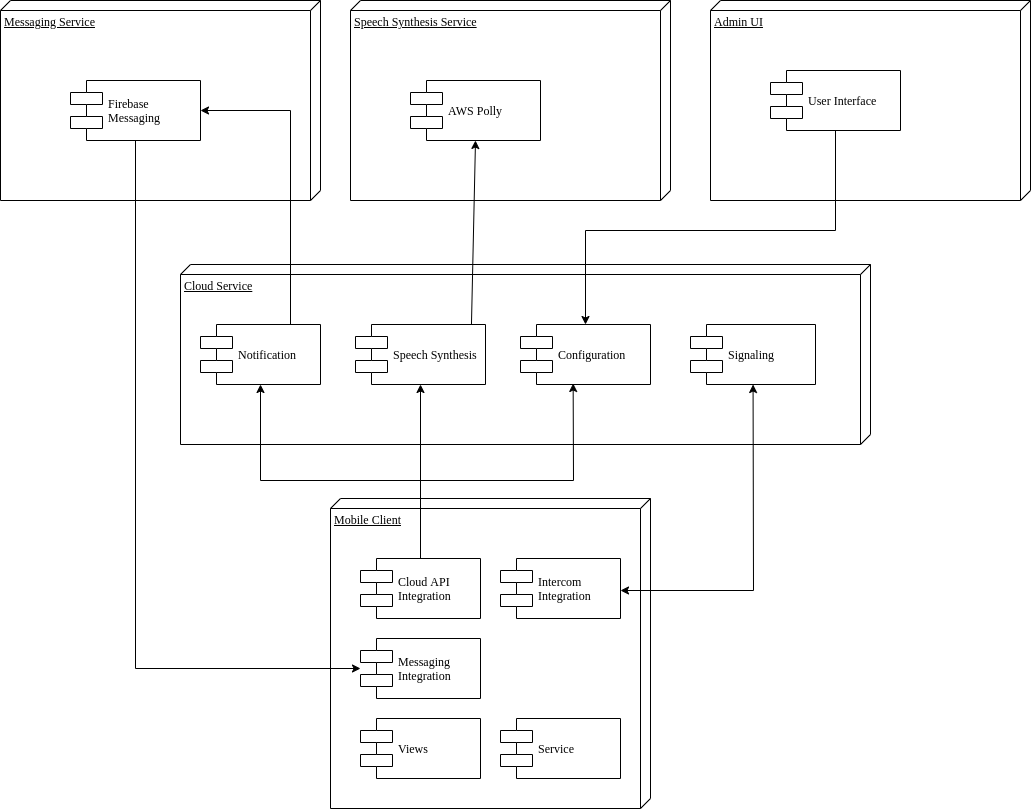
\includegraphics[width=\textwidth]{graphics/diagramms/Component_System_V02}}
        \caption{Systemarchitektur Praxisruf}
    \end{minipage}
\end{figure}

Sprachverbindungen zwischen Mobile Clients werden als Peer To Peer Verbindungen aufgebaut.
Diese Verbindungen wurden mit der Technologie WebRTC umgesetzt.
WebRTC steht für Web Real-Time Communication.
Dabei handelt es sich um ein Open Source Projekt, welches Echtzeitkommunikation für mobile Applikationen und Browser Applikationen ermöglicht.
Damit Peer To Peer Verbindungen zwischen Mobile Clients aufgebaut werden können, müssen diese Meldungen austauschen können.
Um dies zu ermöglichen, wurde der Cloudservice um ein Modul ''Signaling'' erweitert.
Dieses Modul bietet eine Websocketschnittstelle, über welche die nötigen Signalmeldungen ausgetauscht werden können.
Jeder Mobile Client der für Sprachverbindungen verfügbar ist, baut bei der Anmeldung eine Websocketverbindung zum Signaling Modul auf.
Über diese Verbindung sendet und empfängt er alle Signalmeldungen, die für den Verbindungsaufbau notwendig sind.

Im folgenden Bericht werden die erarbeiteten Konzepte und Resultate vorgestellt.
Zunächst werden Vorgehensweise, Projektplan und die Organisation des Projekts vorgestellt.
Anschliessend werden die Anforderungen, welche zu Beginn des Projekts definiert wurden, beschrieben.
Es folgt eine Technologie Evaluation für Sprachsynthese und Gegensprechanlage.
Dabei werden mögliche Optionen beschrieben und anschliessend eine begründete Entscheidung beschrieben.
Das darauffolgende Kapitel beschreibt das detaillierte technische Konzept für Funktionsweise und Architektur des Systems.
Es wird beschrieben, wie die Funktionen Gegensprechanlage und Sprachsynthese umgesetzt wurden.
Dabei wird insbesondere darauf eingegangen, wie die bestehende und neue Funktionen im neuen nativen Mobile Client integriert werden.
Weiter werden die notwendigen Abläufe, Kommunikationskanäle und Datenmodelle beschrieben.
Nach dem Konzept werden die Resultate zusammengefasst und die umgesetzten Ansichten des nativen iOS App abgebildet.
Am Ende der Arbeit stehen ein Fazit und Schlusswort mit Empfehlungen für das weitere Vorgehen.

\clearpage

    \section{Vorgehensweise}

Dieses Kapitel beschreibt die Planung des Projekts, welche zu Projektbeginn definiert wurde.
Es wurde ein Projektplan erarbeitet und Meilensteine zur Fortschrittskontrolle erfasst.

\subsection*{Projektplan}

\begin{figure}[h]
    \centering
    \begin{minipage}[b]{\textwidth}
        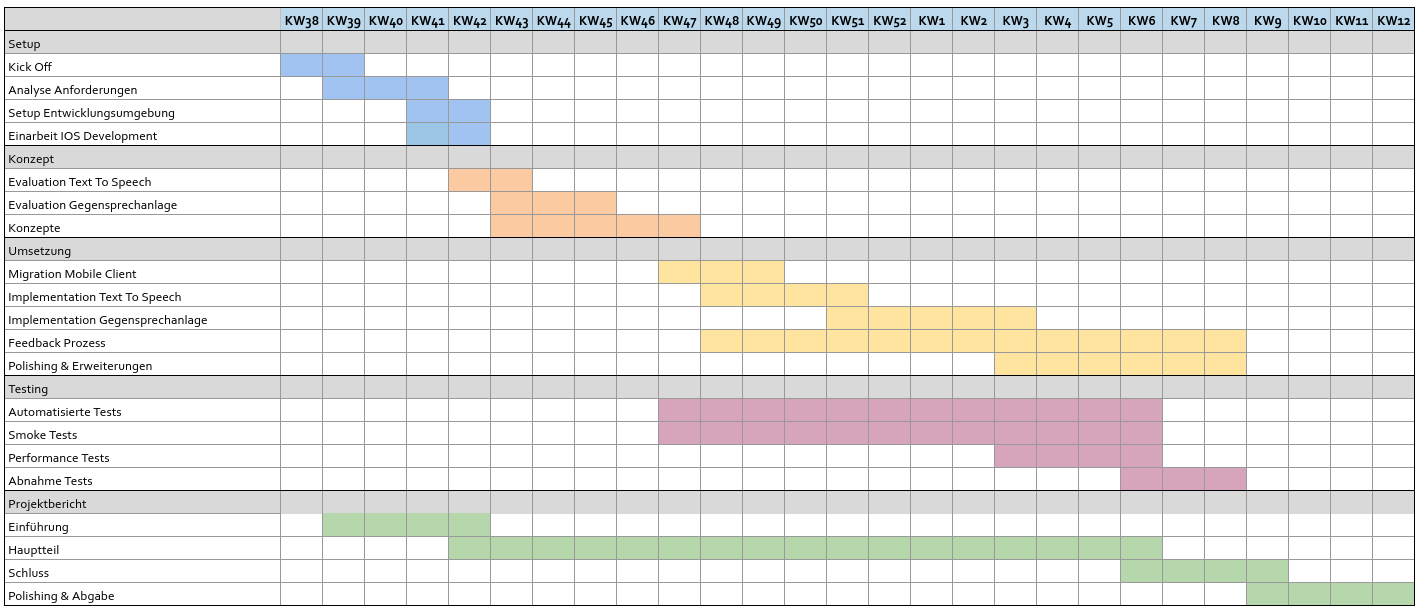
\includegraphics[width=\textwidth]{graphics/projektplan}
        \caption{Projektplan}
    \end{minipage}\label{fig:projektplan}
\end{figure}

Lorem ipsum
\clearpage

\subsection{Meilensteine}

In der Anfangsphase des Projektes wurden folgende Meilensteine definiert:

\begin{table}[h]
    \centering
    \begin{tabular}{|l|p{15cm}|}
        \hline
        \textbf{Id} & \textbf{Beschreibung}                                                                                                                                                                                         \\
        \hline

        M01         & \textbf{Initiale Anforderungsanalyse}

        Die Anforderungen an das Projekt aus der Aufgabenstellungen sind in User Stories dokumentiert.\\
        \hline

        M02         & \textbf{Einarbeit und Setup IOS Umgebung}

        Projektteilnehmende sind mit groben Konzepten der IOS Entwicklung vertraut.
        Die Entwicklungsumgebung ist bereit für die Umsetzung. \\
        \hline

        M03         & \textbf{Evaluation Technologien}

        Die Evaluation der Technologien für Sprachsynthese und Gegensprechanlage ist abgeschlossen. \\
        \hline

        M04         & \textbf{Konzepte}

        Die grundlegenden Konzepte für Systemarchitektur, native iOS Applikation, Gegensprechanlage und Sprachsynthese sind definiert. \\
        \hline

        M05         & \textbf{Migration betehender Funktionalität}

        Die Funktionen die im Mobile Client der Projektarbeit ''IP5 Cloudbasiertes Praxisrufsystem'' umgesetzt wurden, stehen in der neuen iOS Applikation zur Verfügung. \\
        \hline

        M06         & \textbf{Umsetzung Sprachsynthese}

        Die Anforderung zur Funktion Sprachsynthese sind umgesetzt. \\
        \hline

        M07         & \textbf{Umsetzung Gegensprechanlage 1:1}

        Die Anforderung zur Funktion Gegensprechanlage sind für 1:1 Verbindungen umgesetzt. \\
        \hline

        M08         & \textbf{Umsetzung Gegensprechanlage 1:n}

        Die Anforderung zur Funktion Gegensprechanlage sind für 1:n Verbindungen umgesetzt. \\
        \hline

        M09         & \textbf{Polishing und Erweiterungen}

        Die Applikation wurde eingehend getestet.
        Bekannte Fehler sind behoben oder dokumentiert.
        Gewünschte Anpassungen und Erweiterungen sind umgesetzt oder dokumentiert.
        Bei allen nicht umgesetzten Anpassungen ist beschrieben, wieso diese nicht umgesetzt werden konnten.
        \\
        \hline

        M10         & \textbf{Abschluss und Abgfabe}

        Projektbericht und Quellcode sind fertiggestellt.
        Die Projektvereinbarung wurde zeitgemäss abgegeben.\\
        \hline
    \end{tabular}\label{tab:milestones}
\end{table}

\clearpage


    \section{Anforderungen}\label{sec:anforderungen}

Es gibt drei Rollen von Stakeholdern, welche Anforderungen an Praxisruf stellen.
Die meisten Benutzer des Systems fallen in die Rolle Praxismitarbeitende.
Diese verwenden die mobile Applikation von Praxisruf, um in der Praxis miteinander zu kommunizieren.
Neben der Rolle der Praxismitarbeitenden, arbeitet auch die Rolle des Praxisverantwortlichen mit dem Praxisrufsystem.
Diese Benutzergruppe ist dafür verantwortlich, Praxisruf für Praxismitarbeitende zu konfigurieren.
Als dritte Rolle hat zudem der Auftraggeber ein Interesse daran, dass gewisse Rahmenbedingungen gesetzt und eingehalten werden.{Siehe Projektbericht Cloudbasiertes Praxisrufsystem \cite{ip5}}. \\

Im folgenden Kapitel werden die Anforderungen dokumentiert, die bei Projektstart ermittelt wurden.
Die Anforderungen werden dabei aus fachlicher Sicht mit User Stories festgehalten.
Jede User Story beschreibt ein konkretes Bedürniss einer Stakeholdergruppe.

\subsection*{User Stories}

\subsubsection*{Praxismitarbeitende}

\begin{table}[h]
    \centering
    \begin{tabular}{|l|p{15cm}|}
        \hline
        \textbf{Id} & \textbf{Anforderung}                                                                                                                                                                                      \\
        \hline
        U01           & Als Praxismitarbeiter/in möchte ich alle Funktionen aus der existierenden Applikation weiterhin verwenden können, damit mir diese weiterhin die Arbeit erleichtern. \footnote[2]{}                        \\
        \hline

        U02           & Als Praxismitarbeiter/in möchte ich, dass wichtige eingehende Benachrichtigungen vorgelesen werden, damit den Inhalt der Benachrichtigung kenne, ohne meine Aufmerksamkeit auf den Bildschirm zu richten. \\
        \hline
        U03           & Als Praxismitarbeiter/in möchte ich, das Vorlesen von Benachrichtigungen deaktivieren können, damit ich bei der Arbeit nicht unnötig gestört werde.                                                       \\
        \hline
        U04           & Als Praxismitarbeiter/in möchte ich, per Button eine Sprachverbindung zu einem anderen Praxiszimmer aufbauen können, damit ich mich mit einer anderen Person absprechen kann.                             \\
        \hline
        U05           & Als Praxismitarbeiter/in möchte ich, per Button eine Sprachverbindung zu mehreren anderen Praxiszimmern aufbauen können damit, ich mich mit mehreren anderen Personen absprechen kann.                    \\
        \hline
        U06           & Als Praxismitarbeiter/in möchte ich über geöffnete Sprachverbindungen in Echtzeit kommunizieren können damit es die Funktion einer Gegensprechanlage wirklich erfüllt.                                    \\
        \hline
        U07           & Als Praxismitarbeiter/in möchte ich nur Buttons für Sprachverbindungen sehen, die für mich relevant sind.                                                                                                 \\
        \hline
        U08           & Als Praxismitarbeiter/in möchte ich benachrichtigt werden, wenn ein anderes Zimmer eine Sprachverbindung öffnet, damit ich auf die Anfrage Antworten kann.                                                \\
        \hline
        U09           & Als Praxismitarbeiter/in möchte ich vergangene und verpasste Sprachverbindungen nachvollziehen können, damit ich mich zurückmelden kann.                                                                  \\
        \hline
        U10           & Als Praxismitarbeiter/in möchte ich, dass eingehende Sprachverbindungen aus anderen Praxiszimmern automatisch geöffnet werden damit ich meine Hände für besseres brauchen kann.                           \\
        \hline
        U11           & Als Praxismitarbeiter/in möchte ich, direkte Sprachverbindungen aus anderen Praxiszimmern trennen können damit ich ein Gespräch beenden kann.                                                             \\
        \hline
        U12           & Als Praxismitarbeiter/in möchte ich, aus Sprachverbindungen zu mehreren Praxiszimmern (Gruppenunterhaltungen) austreten können, damit ich nicht unnötig bei der Arbeit gestört werde.                     \\
        \hline
    \end{tabular}\label{tab:userstories1}
\end{table}

\clearpage

\subsubsection*{Praxisadministrator}

\begin{table}[h]
    \centering
    \begin{tabular}{|l|p{15cm}|}
        \hline
        \textbf{Id} & \textbf{Anforderung}                                                                                                                                                                                                    \\
        \hline
        U13           & Als Praxisadministrator möchte ich konfigurieren können, welche Benachrichtigungen dem Praxismitarbeitenden vorgelesen werden, damit nur relevante Benachrichtigungen vorgelesen werden.                                \\
        \hline
        U14           & Als Praxisadministrator möchte ich konfigurieren können, aus welchen Zimmern Sprachverbindungen zu welchen anderen Zimmern aufgebaut werden können, damit die Mitarbeitendend das System effizient bedienen können.     \\
        \hline
        U15           & Als Praxisadministrator möchte ich Benachrichtigungen, Clients und Benutzer wie zuvor konfigurieren können, damit ich das System weiterhin auf meine Praxis zuschneiden und bestehende Konfigurationen übernehmen kann. \\
        \hline
    \end{tabular}\label{tab:userstories2}
\end{table}

\subsubsection*{Auftraggeber}

\begin{table}[h]
    \centering
    \begin{tabular}{|l|p{15cm}|}
        \hline
        \textbf{Id} & \textbf{Anforderung}                                                                                                                                                             \\
        \hline
        U16           & Als Auftraggeber möchte ich die bestehende Betriebsinfrastruktur übernehmen, um von der bereits geleisteten Arbeit profitieren zu können.                                        \\
        \hline
        U17           & Als Auftraggeber möchte ich, dass die bestehende Komponenten des Systems wo immer möglich weiter verwendet werden, um von der bereits geleisteten Arbeit profitieren zu können. \\
        \hline
        U18           & Als Auftraggeber möchte ich, der bestehende Mobile Client als native iOS Applikation ungeschrieben wird, um Wartbarkeit und Gerätekompatibilität zu gewährleisten. \\
        \hline
    \end{tabular}\label{tab:userstories3}
\end{table}

\subsection*{Features}

Aus den User Stories ergeben sich drei Features, welche mit dem Projekt "P2P Sprachübertragung in Praxisrufsystemen" umgesetzt werden müssen.

\begin{table}[h]
    \centering
    \begin{tabular}{|l|p{15cm}|}
        \hline
        \textbf{Id} & \textbf{Feature}                                                                                                                                                             \\
        \hline
        F01           & Migration des bestehenden Mobile Client                                        \\
        \hline
        F02           & Text To Speech \\
        \hline
        F03           & Gegensprechanlage \\
        \hline
    \end{tabular}\label{tab:features}
\end{table}

Diese Features dienen zur Aufteilung der Umsetzungsphase.
F01 Migration des bestehenden Mobile Client bildet die Grundalge für die anderen Features und wird deshalb als erstes Umgesetzt.
F02 Text To Speech ist eng mit der bestehenden Funktionalität verbunden.
Es soll deshalb möglichst zeitnah nach F01 umgesetzt werden.
F03 Gegensprechanlage ist das Kernstück der neuen Funktionalität.
Dieses Feature kann erst umgesetzt werden, wenn die Grundlagenarbeit von F01 umgesetzt ist.


\clearpage

    \section{Ausgangslage}

Dieses Kapitel beschreibt das Umfeld in dem diese Projektarbeit ausgeführt wird.
Dabei wird eine grobe Übersicht zu der im Vorgängerprojekt erarbeiteten Lösung gegeben.
Es wird weiter ein Überblick über vergleichbare bestehende Systeme gegeben.

\subsection{Bestehende Rufsysteme}

Im Vorfeld dieses Projektes wurde eine Marktanalyse durchgeführt zu kommerziell erhältlichen Rufsystemen durchgeführt.
Die Resultate dieser Analyse sind in der Aufgabenstellung dieses Projektes zusammengefasst:
Die meisten kommerziell erhältlichen Rufsysteme basieren auf proprietären Standards und setzen veraltete Funktechnologien ein.
Weiter seien bestehende Systeme weder über TCP/IP Netzwerke integrierbar, noch über externe eine API ansteuerbar.\cite{aufgabenstellung}

Durch das Projekt ''IP5 Cloudbasiertes Praxisrufsystem'' wurde ein im Funktionsumfang eingeschränktes cloudbasiertes Praxisrufsystem entwickelt.
Dieses wird im folgenden Kapitel vorgestellt.

\subsection{Vorarbeit Cloudbasiertes Praxisrufsystem}

Das im Projekt ''IP5 Cloudbasiertes Praxisrufsystem'' entwickelte Praxisrufsystem ermöglicht es vorkonfigurierte Benachrichtigungen zwischen Endgeräten zu versenden.
Sprachverbindungen und Sprachsynthese für Benachrichtigungen werden von diesem System nicht unterstützt.

Das bestehende System umfasst eine zentralen Serverkomponente, eine Weboberfläche und eine mobile Applikation.
Die mobile Applikation dient als Endgeräte für Praxismitarbeitende.
Sie ermöglicht es vorkonfigurierte Benachrichtigung zu senden und empfangen.
Die Konfiguration des Systems wird mit der Serverkomponente ''Cloudservice'' verwaltet.
Der Cloudservice bietet dazu eine REST Api an, über welche Konfigurationen erfasst und gelesen werden können.
Diese Api wird von der Weboberfläche ''Admin UI'' angesprochen, um Konfigurationen zu erstellen und bearbeiten.
Sie wird weiter von der mobilen Applikation verwendet, um die Konfiguration der Applikation zu laden.

Das Senden und Empfangen von Benachrichtigungen im bestehenden System wird durch Firebase Cloud Messaging (Firebase Cloud Messaging) ermöglicht.
Sowohl in der Mobile Client als auch im Cloudservice ist eine Anbindung an FCM implementiert.
Dabei wird die Anbindung auf der Seite des Mobile Clients ausschliesslich zum Empfangen von Meldungen verwendet.
Das Versenden von Benachrichtigungen wird an den Cloudservice delegiert.
Dazu sendet ein Mobile Client eine Anfrage an die REST Api des Cloudservice.
Dieser wertet die Konfiguration aus und benutzt die FCM Anbindung um eine Benachrichtigung an alle relevanten Empfänger zuzustellen.

Sämtliche Infrastruktur für das bestehende Praxisrufsystem ist mit Amazon Webservices (AWS) eingerichtet.
Der Cloudservice besteht aus einer einzelnen Java-Applikation.
Diese wird mit einer AWS Elastic Beanstalk Instanz betrieben.
Das Admin UI ist eine simple Javascript Applikation.
Sie wird mit AWS Amplify betrieben.\cite{ip5}

%\subsection{Vergleichbare Anwendungen}
%
%Wie in Kapitel 4.1 beschrieben, gibt es keine kommerziell erhältlichen, cloudbasierte Praxisrufsysteme.
%Es gibt allerdings andere Anwendungen, welche ähnliche Technologien einsetzten und ähnliche Probleme lösen.
%Dieses Kapitel beschreibt, wie diese Sprachübertragung und Sprachsynthese lösen und zeigt auf, wieso diese Lösungen sich nicht als Praxisrufsystem eignen.
%
%\subsubsection{Sprachübertragung}
%
%Die zentrale Aufgabenstellung dieses Projektes dreht sich um die Integration von Sprachverbindungen in ein cloudbasiertes Praxisrufsystem.
%Als Endgerät dafür dienen iOS Tablets.
%
%
%
%
%Sprachverbindungen in mobilen Geräten sind weit verbreitet.
%Neben traditionellen
%
%Gibt keine cloudbasierten oder mobile applikation basierten.
%Am nächsten kommen meeting applikationen, telefon oder chat apps wie whatsapp und discord.
%Ganz andere anforderungen.
%Lange gespräche, Chats etc.
%
%WebRTC ist weit verbreitet und wird von fast allem grossen im Hintergrund verwendet.
%''https://bloggeek.me/massive-applications-using-webrtc/''
%
%\subsubsection{Sprachsynthese}
%Ist schwer.
%Macht man nicht selbst.
%Wird ganz viel als Service angeboten.
%Evaluation beschäftigt sich mit welcher anbieter.
%Konzept beschäftigt sich mit effizienter einbindung.
%
%\subsubsection{Mobile Client}
%Native Apps gibts viele.
%Aber keine die Praxisruf können.
%Wichtigste Anforderungen hier sind, dass bestehende Funktionen unterstützt werden.
%und dass Technologien für t2s und p2p technologie unterstützt werden.

\clearpage


    \section{Technologieentscheid}

In diesem Kapitel wird entschieden, mit welchen Technologien und Frameworks die Anforderungen für das Projekt umgesetzt werden.
Dies beinhaltet die Neuentwicklung des bestehenden Mobile Clients als native iOS Applikation, sowie die Implementation der Features Sprachsynthese und Gegensprechanlage.


\subsection{IOS App}

Mit dem Projekt ''IP5 Cloudbasiertes Praxisrufsystem'' eine mobile Applikation entwickelt, die als Endpunkt in einem Praxisrufsystem verwendet werden kann.
Diese unterstützt das Senden und Empfangen vorkonfigurierter Benachrichtungen~\cite{ip5}.
Die Applikation wurde auf Basis des Frameworks Nativescript~\cite{nativescript} als Multi-Platform Applikation entwickelt.
Dadurch ist es möglich dieselbe Codebasis für die Entwicklung von Android und iOS Applikationen zu verwenden.
Im Fazit des Vorgängerprojekts wurde empfohlen, diese Applikation durch native Applikationen pro Platform zu ersetzten.
Dadurch könne effiziente Weiterentwicklung, sowie Hardware- und Betriebssystemkompatibilität langfristig gewährleistet werden~\cite{ip5}.

Mit diesem Projekt wird die Applikation deshalb neu als native iOS Applikation umgesetzt.
Dabei ist es wichtig, dass sämtliche bestehende Funktionalität auch im neu entwickelten nativen Mobile Client zur Verfügung steht.
Um weiterhin Benachrichtungen senden und empfangen zu können, muss die gewählte Technologie es ermöglichen Firebase Cloud Messaging anzubinden
und Push Benachrichtigungen im Vorder- sowie im Hintergrund empfängen können.
Weiter muss die Technologie es ermöglichen, regelmässige Aufaben auszuführen.
Dadurch kann überprüft werden, ob der Benutzer ungelesene Benachrichtigungen hat und wenn nötig einen Erinnerung dafür angezeigt werden.

\subsubsection{Programmiersprache}

Für die Entwicklung von nativen iOS Applikationen ist die Programmiersprache Swift Industriestandard~\cite{ios_swift}.
Der native iOS Client für Praxisruf wird deshalb mit Swift implementiert.

\subsubsection{Frameworks}

Für die Umsetzung von iOS Applikationen stellt Apple die zwei Frameworks UIKit~\cite{ios_uikit} und SwiftUI~\cite{ios_swift_ui} zur Verfügung.
UIKit ist das ältere der beiden Frameworks und ist seit iOS 2.0 verfügbar.
Dementsprechend ist das Framework ausgereift und bietet viele Funktionen zur Integration einer Applikation mit iOS~\cite{ios_uikit}.

SwiftUI ist deutlich neuer und steht seit iOS 13.0 zur Verfügung~\cite{ios_swift_ui}.
Apple wirbt auf der offiziellen Dokumentationsseite für SwiftUI und schreibt: "SwiftUI helps you build great-looking apps across all Apple platforms with the power of Swift — and as little code as possible."~\cite{ios_swift_ui}
SwiftUI fokussiert sich auf eine declarative Syntax und ist dadurch leichtgewichtiger als UIKit.
Es bietet zudem ausgezeichnete Integration in die XCode Entwicklungsumgebung und viele Standardkomponenten wie Listenansichten, Formfelder und andere UIKomponenten.~\cite{ios_swift_ui}.
Dadurch wird es einfacher eine Benutzeroberfläche mit nativem Look und Feel einer iOS Applikation umzusetzten.

Da SwiftUI deutlich neuer ist als UIKit, ist es möglich das es noch nicht alle Funktionen und Betriebssystem Integrationen unterstützt die in UIKIt möglich sind.
Dieses Problem wird dadurch aufgehoben, dass UIKit Funktionen nahtlos in SwiftUI integriert werden können.\cite{ios_swift_ui_uikit}
Es ist also grundsätzlich möglich, alles was mit UIKit umgesetzt werden kann auch mit SwiftUI umuzusetzen.

\clearpage

\subsubsection{Unterstützung Benachrichtigungen}

Die neue iOS Applikation, muss es weiterhin ermöglichen Benachrichtigungen über Firebase Cloud Messaging zu empfangen und versenden.
Firebase stellt dazu eine native iOS Library zur Verfügung~\cite{firebase_github_ios}.
Die Integration von Firebase Cloud Messaging kann mit dieser Library implementiert werden.
Dies beinhaltet die Registrierung bei Firebase Cloud Messaging, sowie das Empfangen der Benachrichtigungen über Firebase~\cite{firebase_ios}.
Damit Push-Benachrichtigungen über das Betriebssystem angezeigt werden können, müssen empfangene Benachrichtigungen an das Betriebssystem übergeben werden.
Mit sogenannten AppDelegates ist es möglich sich in den Lifecycle des Betriebssystems einzuhängen~\cite{ios_app_delegate}.
Dadurch ist es auch möglich, Vorder- und Hintergrundbenachrichtigungen über das Benachrichtigungszenter von iOS anzuzeigen~\cite{firebase_ios}.

Die Firebase Cloud Messaging Library kann sowohl mit SwiftUI als auch mit UIKit verwendet werden.
AppDelegates sind ein Konzept welches aus UIKit stammt\cite{ios_app_delegate}.
SwiftUI Applikationen können ohne AppDelegates implementiert werden.
UIKit Funktionen können allerdings nahtlos mit SwiftUI integriert werden.\cite{ios_swift_ui_uikit}
Die Firebase Cloud Messaging Library für iOS ermöglicht es also, Benachrichtigungen von Praxisruf sowohl mit UIKit als auch mit SwiftUI umzusetzten.

Um Konfigurationen zu laden und Benachrichtigungen zu versenden, muss die REST Api des Cloudservice angesprochen werden können.
Dies ist über die URLRequest-Komponente aus der iOS Standardbibliothek möglich~\cite{ios_urlrequest}.

\subsubsection{Benachrichtigungen prüfen}

Die mobile Applikation aus dem Vorgängerprojekt erinnert in regelmässigen Abständen, wenn ungelesene Benachrichtigungen vorhanden sind.
Diese Funktion muss auch von der neuen iOS Applikation unterstützt werden.
Dazu muss regelmässig geprüft werden, ob es ungelesene Benachrichtigungen gibt und gegebenenfalls ein Erinnerungston abgespielt werden.
Die standard iOS Bibliothek bietet Mittel, mit welchen regelmässige Aufgaben angestossen werden können.
Einerseits können über eine ''Timer''-Komponente in Regelmässigen abständen Events veröffentlicht werden.
Auf einer SwiftUI View kann ein beliebiger Listener registriert werden, der beim Empfang eines Events des Timers aufgerufen wird.
Dies bringt die Einschränkung mit sich, dass die Prüfung nur ausgeführt ist, wenn die App im Vordergrund läuft und die View geladen wurde~\cite{ios_timer}.
Da der bestehende Mobile Client dieselbe Einschränkung hat, könnte mit einem Timer trotzdem genau dasselbe Verhalten wie in der bestehenden Applikation umgesetzt werden.
Die Standardbibliothek bietet allerdings auch Mittel, um Aufgaben im Hintergrund zu verarbeiten.
Über die Klasse BGTaskScheduler können Aufgaben erfasst werden, die im Hintergrund ausgeführt werden~\cite{ios_bgtaskscheduler}.

Die Erinnerungsfunktion kann mit Mitteln aus der iOS Standardbibliothek umgesetzt werden.

\subsubsection{Entscheid}

Der native iOS Mobile Client für Praxisruf wird mit Swift und SwiftUI umgesetzt.
Die deklarative Syntax von SwiftUI, ermöglicht es einfacher übersichtliche und lesbare Komponenten zu implementieren.
Integration in die XCode Entwicklungsumgebung und verfügbare Standardkomponenten vereinfachen die Entwicklung.
Es ist möglich, dass einige Funktionen noch nicht mit SwiftUI umgesetzt werden können, weil dafür benötigte Features noch nicht unterstützt werden.
Da UIKit Funktionen nahtlos in SwiftUI integriert werden können, ist es möglich betroffene Teile der Applikation mit UIKit zu implementieren.
Diese Teile können, sobald die entsprechenden Funktionen in SwitUI verfügbar sind, migriert werden.

Als Zielplattform für die Applikation wird iOS15 verwendet.
Damit wird die neuste iOS Version unterstützt.
Dies ermöglicht es, alle verfügbaren SwiftUI Features zu verwenden und minimiert die Wahrscheinlichkeit, auf UIKIt zurückgreifen zu müssen.

\clearpage

\subsection{Sprachsynthese}

Das Feature Sprachsynthese fordert, dass das System das Vorlesen empfangener Benachrichtigungen unterstützt.
Um dies zu ermöglichen muss eine Technologie integriert werden, die es erlaubt aus Sprachdaten aus Textinhalten zu synthetisieren.
Diese Sprachdaten müssen als Audiodateien vom Mobile Client abgespielt werden können.

Diese Integration kann mit den Standardbibliotheken für iOS oder durch die Anbindung eines externen Providers umgesetzt werden.
Die Anbindung eines externen Providers kann direkt im Mobile Client implementiert werden.
Alternativ kann die Serverkomponente Cloudservice an den Provider angebunden werden und allen Clients eine einheitliche Schnittstelle bieten, um diese Daten abzufragen.

\subsubsection{Apple Speech Synthesis}

Die iOS Standardbibliothek bietet Komponenten zur Konvertierung von Text zu Sprache~\cite{ios_speech_synthesis}.
Die Verwendung dieser Komponenten verspricht zwei Vorteile:
Erstes kann Sprachsynthese dadurch ohne die Anbindung eines Drittanbieters umgesetzt werden.
Zweitens ist die Kompatibilität mit iOS15 Clients garantiert und die Integration der Funktionen ohne externe Bibliotheken möglich~\cite{ios_speech_synthesis}.
Gleichzeitig entsteht damit aber eine starke Bindung an Apple als Dienstleister für Sprachsynthese.
Sollte die Funktion in künftigen Versionen nicht mehr unterstützt werden, müsste die ganze Integration von Sprachsynthese neu evaluiert und implementiert werden.
Weiter reduziert diese Variante die Flexibilität der Systemarchitektur.
Mit der Verwendung der iOS Standardbibliothek für Sprachsynthese, muss die Anbindung an den Dienstleister direkt in der iOS Applikation umgesetzt werden.
Dies ist insbesondere ein Nachteil, da für dieselbe Funktionalität in zukünftigen Android Clients ein anderer Dienstleister verwendet werden muss.
Eine einheitliche Integration der Sprachsynthese in zukünftigen Plattformen ist deshalb nicht möglich, wenn Apple Speech Synthesis verwendet wird.

\subsubsection{Amazon Polly}

Vom Auftraggeber ist explizit gewünscht, dass für Infrastruktur und Dienstleistungen wo möglich Amazon Webservices verwendet wird\footnote{Siehe Kapitel 3.1.3}.
Mit dem Amazon Polly bietet Amazon Webservices einen Service, welcher Text in Sprachdaten verwandeln kann~\cite{aws_polly}.
Amazon Webservices stellt Libraries für iOS~\cite{aws_polly_ios}, Android~\cite{aws_polly_sdks} und für Java zur Verfügung~\cite{aws_polly_java}.
Polly kann damit sowohl direkt in native mobile Applikationen als auch in den Cloudservice integriert werden.

Die iOS Library von Amazon Polly ermöglicht es, die Anbindung des externen Sprachsyntheseproviders direkt im Mobile Client zu implementieren~\cite{aws_polly_ios}.
Diese Lösung kann für zukünftige Android Clients analog mit der Android Library für Aws Polly umgesetzt werden.
Die starke Bindung zu Apple als Dienstleister für Sprachsynthese entfällt durch diese Lösung.
Es wird allerdings eine starke bindung zu Amazon Polly als Dienstleister geschaffen.
Ein Wechsel des Providers bleibt auch in dieser Variante aufwändig.
Weiter bringt auch diese Variante den Nachteil, dass der Mobile Client komplexer wird, weil er mit einer zusätzlichen Instanz kommunizieren muss.

Mit der Java Bibliothek von Amazon Polly kann die Anbindung des Sprachsyntheseproviders im Cloudservice vorgenommen werden.
Dadurch ist es möglich im Cloudservice eine Schnittstelle zu implementieren, welche den Bezug von Sprachdaten für Benachrichtigungen erlaubt.
Diese Schnittstelle kann in die bestehende API des Cloudservices integriert werden.
Damit können alle Clients die Sprachdaten über dieselbe Schnittstelle beziehen.
Caching von Sprachdaten kann sowohl auf Serverseite als auch auf Clientseite implementiert werden.
Die Integration von Sprachsynthese in die API des Cloudservices ermöglicht es weiter, den gewählten Dienstleister in Zukunft einfach und ohne die Clients anzupassen auszutauschen.
Gleichzeitig hat diese Variante den Nachteil, dass der Cloudservice komplexer wird.
Durch die Integration von Sprachsynthese wird ein neues Umsystem angebunden.
Die Komplexität des Systems als Ganzes, wächst dadurch in jedem Fall.
Wie stark die Komplexität des Systems zunimmt, kann jedoch minimiert werden, indem die neue Funktionalität eng gekapselt wird.
Sie kann so umgesetzt werden, dass sie unabhängig vom restlichen System bleibt und alle nötigen Daten über die Schnittstelle der anderen Module bezieht.

Als dritte Option für die Integration von Amazon Polly kan AWS Lambda verwendet werden~\cite{aws_polly}.
AWS Lambda erlaubt es Funktionalität serverless auszuführen.
Der entsprechende Code läuft in diesem Fall nicht als klassischer Server, sondern wird nur bei Bedarf ausgeführt~\cite{aws_lambda}
Die Integration von Amazon Polly über AWS Lambda kann für das Praxisrufsystem in zwei Verarbeitungsschritten implementiert werden.
In einem ersten Schritt werden die zu synthetisierenden Daten geladen und an Amazon Polly gesendet.
Anschliessend werden die Resultate, die Amazon Polly liefert persistiert.
Die Abfrage von Sprachdaten kann in diesem Fall ebenfalls in die API des Cloudservices integriert werden.
Dazu müssen die persistierten Sprachdaten geladen und zurückgegeben werden.
Die Verwendung von AWS Lambda hat damit den Nachteil, dass die synthetisierten Sprachdaten zwingend ausserhalb des Mobile Clients persistiert werden müssen.
Weiter findet damit eine zusätzliche Bindung an Amazon statt.
Gleichzeitig bietet es den Vorteil, dass weniger Infrastruktur benötigt wird, da die Abfrage an AWS Polly ohne dedizierten Server abgesetzt werden kann.

\subsubsection{Entscheidung}

Die Sprachsynthese wird durch die Anbindung des externen Providers Amazon Polly umgesetzt.
Der Cloudservice übernimmt die Kommunikation mit Amazon Polly und bietet eine Schnittstelle, über welche Clients Audiodaten beziehen können.
Diese Schnittstelle wird in die API des Cloudservices integriert.
Die Anbindung an Amazon Polly wird dabei direkt im Cloudservice implementiert und nicht über AWS Lambda gelöst.

Durch diesen Ansatz wird die Abhängigkeit zu einzelnen Provider minimiert.
Die Anbindung von Sprachsynthese kann für alle Client Plattformen einheitlich umgesetzt werden.
Dies macht diese Variante zukunftssicher und bietet grössere Flexibilität für den Betrieb.
Der Einfluss von zusätzlicher Komplexität, die dieser Ansatz mit sich bringt, wird durch entsprechende Kapselung in der Systemarchitektur minimiert.

\clearpage

\subsection{Gegensprechanlage}

Die zentrale Aufgabenstellung dieser Arbeit dreht sich darum, Peer-To-Peer Sprachübertragung in ein cloudbasiertes Praxisrufsystem zu integrieren.
In diesem Kapitel wird entschieden, welche Technologie zur Umsetzung dieser Aufgabe verwendet wird.
Es werden dabei zwei Ansätze beschrieben, mit welchen diese Anforderung umgesetzt werden kann.
Der erste Ansatz beinhaltet die Anbindung eines externen Anbieters für Kommunikationslösungen.
Der zweite Ansatz verzichtet auf die Integration eines Anbieters und setzt Sprachverbindungen als Peer-To-Peer Verbindungen basierend auf WebRTC um.

\subsubsection{Amazon Chime}

Eine Möglichkeit um Sprachverbindungen in Praxisruf zu implementieren, ist die Integration einer bestehenden Business-Kommunikationslösung, wie Webex oder Microsoft Teams.
Auch für die Integration von Sprachverbindungen gilt, dass für Infrastruktur und Dienstleistungen wo möglich Amazon Webservices verwendet wird\footnote{Siehe Anforderung U19 in Kapitel 3.1.3}.
Mit Amazon Chime bietet Amazon einen Dienst für Telefonie, Chats und Videokonferenzen~\cite{aws_chime}.
Chime bietet einerseits Web- und Mobile Applikationen für Anrufe und Meetings.
Andererseits ist es mit dem Amazon Chime SDK für iOS möglich, Chime in eigene native iOS Applikationen zu integrieren~\cite{aws_chime_sdk}.
Chime ermöglicht es Konferenzunterhaltungen mit bis zu 250 Teilnehmern zu starten~\cite{aws_faq}.
Damit bietet der Anbieter alle benötigte Funktionen um Einzel- und Gruppenunterhaltungen in einem Praxisrufsystem umzusetzen.

Integration eines Providers wie Amazon Chime hat den Vorteil, dass die Telefonie in einen etablierten Provider ausgelagert werden kann.
Durch Verträge mit dem Provider können Verfügbarkeitsgarantien und Supportleistungen vereinbart werden.
Dies erhöht die Stabilität des Systems und ermöglicht effizientes Reagieren im Fehlerfall.
Weiter fallen für Praxisruf selbst wenig bis keine Aufwände für den Betrieb der nötigen Infrastruktur.

Amazon Chime unterstützt deutlich mehr Funktionen als in einem Praxisrufsystem benötigt werden.
Ein Rufsystem muss als Gegensprechanlage verwendet werden können und kurze Gespräche zwischen Teilnehmern erlauben.
Dies bedeutet einerseits, dass Chime garantiert alle Funktionen bietet welche benötigt werden.
Es bedeutet aber andererseits auch, dass nur ein kleines Subset der vorhandenen Möglichkeiten ausgenutzt wird.
Ein Nachteil daran ist, dass eine starke Bindung an Amazon und die Abläufe, die Amazon Chime zum Verbindungsaufbau vorsieht, stattfindet.
Gleichzeitig kann von vielen Vorteilen von Amazon Chime nicht profitiert werden, weil die entsprechenden Funktionen für ein Praxisrufsystem nicht relevant sind.

\subsubsection{WebRTC}

WebRTC (Web Real-Time Communication) ermöglicht Echtzeitkommunikation basierend auf einem offenen Standard.
Das Open-Source-Projekt wird unter anderem von Apple, Google, Microsoft und Mozilla unterstützt.
Es erlaubt den Austausch von Sprach-, Video- und allgemeinen Daten zwischen Clients.
Wie auf der offiziellen Webseite von WebRTC beschrieben stehen die Technologien
''[\ldots] in allen gängigen Browsern als reguläre JavaScript-APIs verfügbar.
Für native Clients wie Android- und iOS-Anwendungen steht eine Bibliothek zur Verfügung, die dieselben Funktionen bietet.''~\cite{webrtc}.

WebRTC baut zur Kommunikation direkte Peer-To Peer-Verbindungen zwischen den Kommunikationspartnern auf.
Die WebRTC Libraries und APIs bieten Komponenten für die Integration von Peer-To-Peer Verbindung, Hardwarezugriff auf Microphon und Kamera.
WebRTC spezifiziert allerdings nicht, wie für den Verbindungsaufbau notwendige Informationen zwischen Teilnehmern ausgetauscht werden müssen.
Um den Austausch diese Informationen zu ermöglichen ist eine Signaling Instanz notwendig.
Die Signaling Instanz muss es ermöglichen, Informationen zwischen Teilnehmern zu vermitteln.
WebRTC spezifiziert nicht, wie diese Signaling Instanz aussehen muss.
Neben der Signaling Instanz ist keine weitere Infrastruktur notwendig.
Sämtliche Daten werden direkt über die Peer-To-Peer Verbindungen zwischen Clients ausgetauscht.

Dies hat den Vorteil, dass die Abhängigkeit zu externen Umsystemen minimiert werden kann.
Der Signaling Service kann auf die eigenen Anforderungen zugeschnitten werden.
Die Technologie über welche Signale ausgetauscht werden, kann frei gewählt werden.
Signaling für Sprachverbindungen im Praxisrufsystem kann damit in den Cloudservice integriert werden.
So kann notwendige Infrastruktur, die als Teil des Praxisrufsystems betrieben werden muss, schlank gehalten werden.
Die Integration der Signalvermittlung in den Cloudservice bietet weiter den Vorteil, dass bestehende Funktionen des Systems angesprochen werden können.
So können z.B. \ Benachrichtigung bei verpassten Anrufen über die bereits umgesetzte Benachrichtigungsfunktion versendet werden.

Die Verwendung von WebRTC hat den Nachteil, dass kein fachlicher Support bei Verbindungsproblemen zur Verfügung steht.
Signaling Instanz und Implementation der Sprachverbindungen stehen in der alleinigen Verantwortung des Betreibers des Praxisrufsystems.
Abgesehen von Fehlern in der Implementation können Verbindungsprobleme an zwei Stellen auftreten.
Einerseits ist es möglich, dass die Signaling Instanz ausfällt und nicht erreichbar ist.
Dieses Problem kann durch den Betrieb des Cloudservice adressiert werden.
Die Signaling Instanz kann in den Cloudservice integriert werden.
Dieser wird wiederum bei einem Cloud-Provider betrieben.
Für diesen Betrieb können Verträge definiert werden, die Verfügbarkeit und Support im Fehlerfall bieten.
Andererseits können lokale Netzwerkprobleme auftreten, welche Endgeräte unerreichbar machen.
Dieses Problem besteht unabhängig davon, wie Sprachübertragung implementiert wird.
Im Fall des Praxisrufsystems kann das Problem dadurch adressiert werden, dass nicht erreichbare Endgeräte durch asynchrone Benachrichtigungen über verpasste Verbindungen informiert werden.

Die Gegensprechanlage in einem Praxisrufsystem muss Verbindung mit mehreren Teilnehmern gleichzeitig erlauben.
Verbindungen müssen deshalb als zwischen zwei Teilnehmern als 1:1 Verbindungen, aber auch zwischen mehreren Teilnehmern als 1:n Verbindungen umgesetzt werden.
WebRTC sieht ausschliesslich direkte Peer-To-Peer Verbindungen vor.
Es ist allerdings möglich, mehrere direkte Peer-To-Peer Verbindungen gleichzeitig zu verwenden~\cite{webrtc_mesh}.
Weiter ist es möglich, die Kommunikation über eine zentrale Instanz zu bündeln.
Eine solche nennt sich Multipoint Conferencing Unit (MCU).
Bei der Verwendung einer MCU werden Verbindungen nicht direkt zwischen Endgeräten hergestellt.
Stattdessen stellt jedes Endgerät eine Verbindung mit der MCU her.
Die MCU vermittelt die Daten zwischen allen Teilnehmern.
Die Verwendung einer MCU verkompliziert das System und die benötigte Infrastruktur massgeblich~\cite{webrtc_mcu}.

\subsubsection{Entscheidung}

Sprachverbindungen für die Funktion Gegensprechanlage werden mit WebRTC umgesetzt.
Der Cloudservice wird um ein Modul erweitert, welches als Signaling Instanz dient.
Die WebRTC iOS Bibliothek wird verwendet, um Peer-To-Peer Sprachübertragung in einer nativen iOS App zu implementieren.

Durch die Verwendung von WebRTC, können Sprachverbindungen aufgebaut werden, ohne ein weiteres Drittsystem anzubinden.
Die benötigte Infrastruktur kann dadurch auf ein Minimum reduziert werden.
Eine eigene Implementierung der Signaling Instanz ermöglicht es weiter, bestehende Funktionen des Praxisrufsystems effizient zu verwenden.
Die Verfügbaren Libraries für iOs, Android und Javascript bedeuten, dass künftige Web- und Android Clients in das System integriert werden können.
Die Verfügbarkeit der Signaling Instanz wird den Betrieb des Cloudservices sichergestellt.

\clearpage


    
\section{Technische Grundlage}

Beschreibt die theoretische Grundlage für die verwendeten Technologien.
Was ist grundsätzlich notwendig, um das in ein Praxisrufsystem zu integrieren.

\subsection{Peer-To-Peer Sprachübertragung}

Was braucht WebRTC um P2P aufzubauen.
Was sind die iOS Spezifischen Komponenten.
Was bedeutet das für Praxisruf.
Übertragungsprotokolle und sicherheit.

\subsection{Sprachsynthese}

Was braucht es um AWS Polly zu integrieren.
Lambda und ähnliches ist Provider spezifisch.
Schnittstelle in Cloudservice ist besser.
Übertragungsprotokolle und sicherheit.
%''https://docs.aws.amazon.com/polly/latest/dg/encryption-in-transit.html''

\subsection{Native iOS Applikation}

Muss die Anbindung an Umsysteme implementieren.
Umsysteme sind Messaging Service, Cloud Service.
Weiter müssen die Komponenten für P2P Verbindungen zu anderen Geräten geschrieben werden.
Verbindungsmanagement und UX.
Übertragungsprotokoll und Sicherheit FCM.

\clearpage


    \section{Konzept}

Dieses Kapitel beschreibt das Konzept, nach welchem das cloudbasierte Praxisrufsystem aus dem Vorgängerprojekt erweitert wurde.
Die Konzepte wurden vor Beginn der Umsetzung definiert und während der Umsetzung laufend überarbeitet.
Die folgende Dokumentation beschreiben die neuste Version des Konzepts und stellen damit das umgesetzte System dar.
Dabei wird nicht hervorgehoben, welche Teile zu Beginn definiert und welche Teile später überarbeitet oder ergänzt wurden.

Das Konzept gibt zuerst einen Überblick über das System als Ganzes.
Es werden die einzelnen Teile des Systems beschrieben und es werden Schritte definiert, um die Weiterentwicklung des Systems zu vereinfachen.
Nach dem Systemkonzept werden Konzepte für die Umsetzung der drei Features ''Migration des bestehenden Mobile Client'', ''Sprachsynthese'' und ''Gegensprechanlage'' beschrieben.
Das Kapitel schliesst mit einem Überblick über die Domänen- und Servicemodelle sowie der Schnittstellen welche die API des Systems bietet.


\subsection{Systemarchitektur}

Dieses Kapitel beschreibt die Komponenten des Praxisrufsystems und wie diese erweitert werden.
Das System wird um Komponenten zur Signalvermittlung und Sprachsynthese erweitert.
Weiter wird die interne Struktur des Cloudservices angepasst um die Weiterentwicklung und Betrieb des Systems zu vereinfachen.

\begin{figure}[h]
    \centering
    \begin{minipage}[b]{0.8\textwidth}
        \fbox{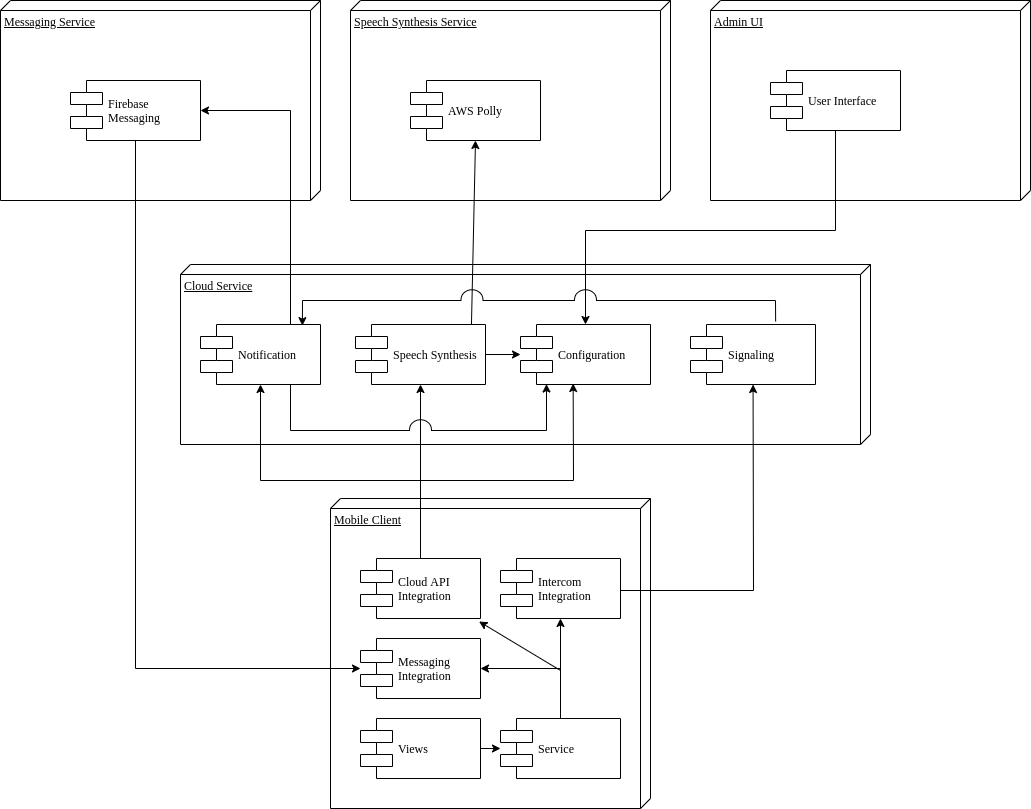
\includegraphics[width=\textwidth]{graphics/diagramms/Component_System_V03}}
        \caption{Systemkomponenten}
    \end{minipage}
\end{figure}

Abbildung 7.1 gibt einen Überblick über die Systemkomponenten und welche Teile diese beinhalten.
Die Pfeile zwischen Komponenten zeigen gerichtete Abfragen und damit eine Funktionale Abhängigkeit.
Alle dargestellten Komponenten sind entkoppelt und Abfragen finden nur über definierte Schnittstellen statt.

\subsubsection{Systemkomponenten}

Dieses Kapitel beschreibt die in Abbildung 7.1 abgebildeten Systemkomponenten.
Dabei wird für jede Komponente beschrieben, welche Aufgaben ihr zufallen und wie sie im Rahmen dieses Projektes erweitert wird.

\textbf{Cloudservice}

Der Cloudservice bildet das zentrale Serverkomponente des Praxisrufsystems.
Zu Beginn dieses Projektes umfasst der Cloudservice die beiden Domänen Notification und Configuration.
Dabei ist die Domäne Notification für das Versenden von Benachrichtigungen und die Domäne Configuration für die Verwaltung und Auswertung der Konfigurationen verantwortlich.
Die relevanten Empfänger für eine Benachrichtigung werden in der Configuration Domain ermittelt.
Um auf diese Informationen zugreifen zu können, muss aus der Notification Domain eine Abfrage an die Configuration Domain geschehen.
Die Configuration Domäne bietet dazu eine REST Schnittstelle~\cite{ip5}.

Die Trennung der Domänen wurde im Vorgängerprojekt lediglich auf Package-Ebene realisiert.
Mit diesem Projekt soll die Trennung einen Schritt weiter gehen.
Der Cloudservice wird Module aufgeteilt.
Diese Module werden weiterhin in einer einzelnen Applikation zusammengefasst.
Die Modularisierung können aber zu einem späteren Zeitpunkt in einzelne Microservices aufgeteilt werden.

Nachdem die Auftrennung in Module stattgefunden hat, wird der Cloudservice um die zwei Module Signaling und Speech Synthesis erweitert.
Das neue Modul Signaling ist für die Signalvermittlung zwischen Mobile Clients verantwortlich.
Es übernimmt die Aufgabe der Signaling Instanz für den Aufbau von Peer-To-Peer Sprachverbindungen mit WebRTC.
Das Modul Signaling hat eine gerichtete Abhängigkeit zum Module Notification.
Über das Notification Modul sollen Empfänger informiert werden, wenn ein Signal nicht zugestellt werden konnte.
Das neue Modul Speech Synthesis dient als Schnittstelle zu einem externen Provider für Sprachsynthese.
Dies ermöglicht es, die Sprachsynthese als Teil der API des Cloudservice anzubieten.
Dadurch können Clients aller Plattformen und auch Systeme, die künftig angebunden werden, auf die Sprachsynthese zugreifen.
Weil alle Clients die Daten aus derselben Schnittstelle beziehen, ist garantiert, dass die Konfiguration und Funktionsweise dieselbe für alle Clients ist. \\

\textbf{Mobile Client}

Der Mobile Client ist eine mobile Appliaktion, über welche das Praxisrufsystem bedient werden kann.
Der mit dem Vorgängerprojekt umgesetzte Mobile Client erlaubt es Benachrichtigungen zu versenden und empfangen~\cite{ip5}.
Dieser Mobile Client wird durch eine native iOS Applikation ersetzt.
Die native iOS App wird von Grund auf neu entwickelt.
Dabei muss sämtliche Funktionen des bestehenden Mobile Clients als Teil der nativen App neu implementiert werden.
Weiter werden die Funktionen Gegensprechanlage und Sprachsynthese für empfangene Benachrichtigungen umgesetzt.

\textbf{Admin UI}

Das Admin UI ist eine Webapplikation, über welche die Konfiguration des Praxisrufsystems verwaltet werden kann.
Die Konfiguration des Systems wird für Gegensprechanlage und Sprachsynthese erweitert.
Für die Gegensprechanlage müssen Buttons konfiguriert werden können.
Diese beinhalten Anzeigetext und Teilnehmer einer Sprachverbindung.
Weiter muss pro Benachrichtigung konfigurierbar sein, ob ihr Inhalt bei Empfang vorgelesen werden sollen.
Das Admin UI muss erweitert werden, um die Verwaltung der erweiterten Konfiguration zu ermöglichen.

\textbf{Messaging Service}

Der Messaging Service ist für die Zustellung von Push Benachrichtigungen an Mobile Clients verantwortlich.
Der Cloudservice muss an den Messaging Service angebunden sein, um Benachrichtigungen anhand der Konfiguration zu versenden~\cite{ip5}.
Die Anbindung des Cloudservices an den Messaging Service ist mit dem Vorgängerprojekt bereits umgesetzt und muss für dieses Projekt nicht angepasst werden.
Die neu entwickelte native iOS App muss hingegen an den Messaging Service angebunden werden, um Benachrichtigungen zu empfangen.
Als Messaging Service wird Firebase Cloud Messaging verwendet.

\textbf{Speech Synthesis Service}

Um Sprachsynthese zu ermöglichen, wird ein externer Service angebunden.
Dieser übernimmt die Konvertierung von Text aus Benachrichtigungen zu Sprachdaten.
Die Anbindung an den Speech Synthesis Service wird ausschliesslich im Cloudservice implementiert.
Sämtliche andere Komponenten die Sprachdaten benötigen, fragen diese beim Cloudservice ab.
Die REST API des Cloudservice wird um entsprechende Endpunkte erweitert.
Als Speech Synthesis Service wird Amazon Polly verwendet.

\subsubsection{Modularisierung Cloudservice}

Der mit dem Vorgängerprojekt umgesetzte Cloudservice ist als monolithische Applikation implementiert.
Er trennt intern die beiden Domänen Notification und Configuration.
Die Domäne Configuration ist für die Verwaltung und Auswertung der Konfiguration des Systems und die Domäne Notification für das Versenden von Benachrichtigungen verantwortlich.
Abhängigkeiten zwischen den beiden Domänen ist über eine REST-Schnittstelle abstrahiert.

Die Trennung der Domänen, erlaubt es die Anwendung zukünftig in mehrere Microservices aufzuteilen.
Diese könnten unabhängig betrieben und erweitert werden.
Weiter wird es dadurch möglich, einzelnen Teilen der Applikation mehr Ressourcen zuzuteilen.
Die Trennung der Domänen in eigene Microservices wurde noch nicht vorgenommen.
Die beiden Domänen wurden lediglich durch die Package Struktur innerhalb eines einzelnen monolithischen Services getrennt.

Die Trennung der Domänen innerhalb des Cloudservice wird weiter verstärkt.
Teile der Applikation werden neu in Module aufgeteilt.
Dabei wird pro Domäne ein Modul erstellt.
Dieses kapselt sämtliche Domänenobjekte, Services und Schnittstellen der jeweiligen Domäne.
Dadurch ist garantiert, dass die Domänen sauber voneinander getrennt sind.
Sämtliche Kommunikation zwischen den Modulen muss über REST-Schnittstellen geschehen.

Es werden die vier Domänen-Module Configuration, Notification, Spech Synthesis und Signaling definiert.
Das Modul Configuration beinhaltet alle Domänenobjekte, Services und Schnittstellen für die Verwaltung, Auswertung und Abfrage der Systemkonfiguration.
Das Modul Notification beinhaltet alle Domänenobjekte, Services und Schnittstellen für das Versenden von Benachrichtiungen.
Das Modul Speech Synthesis beinhaltet die Anbindung an den Speech Synthesis Service und stellt eine Schnittstelle zur verfügung über den das restliche System Sprachdaten beziehen kann.
Das Modul Signaling beinhaltet Domänenobjekte, Services und Schnittstellen für die Signalvermittlung zwischen Mobile Clients.

Weiter werden die zwei Module Commons und App definiert.
Komponenten, welche in mehr als einer Domäne verwendet werden, werden in ein zusätzliches Commons Modul verlegt.
Dazu gehören Data Transfer Objects für Schnittstellen zwischen den Modulen, geteilte Clients um Abfragen auf andere Module abzusetzen sowie Komponenten für Security und Fehlerhandling.
Neben den Modulen App und Commons, werden vier weitere Module für die Domänen Configuration, Notification, Speech Synthesis und Signaling erstellt.

Der Cloudservice wird weiterhin als monolithische Applikation betrieben.
Die Modularisierung garantiert dabei eine strikte Trennung der Domänen.
In Zukunft können einzelne Module aus dem Cloudservice ausgelöst und als eigenständige Applikationen betrieben werden.

\clearpage

\subsubsection{Domänenmodell Cloudservice}

Das Domänenmodell Cloudservices wird für die Integration von Sprachsynthese und Gegensprechanlage erweitert.
Abbildung 7.2 gibt eine Übersicht über das vollständige Domänenmodell der Domänen Configuration und Notification.
Die neuen Domänen Speech Synthesis und Signaling führen keine persistierten Daten.
Die Services und Komponenten dieser Domänen sind in den Kapiteln 7.3 und 7.4 beschrieben.

\begin{figure}[h]
    \centering
    \begin{minipage}[b]{0.9\textwidth}
        \fbox{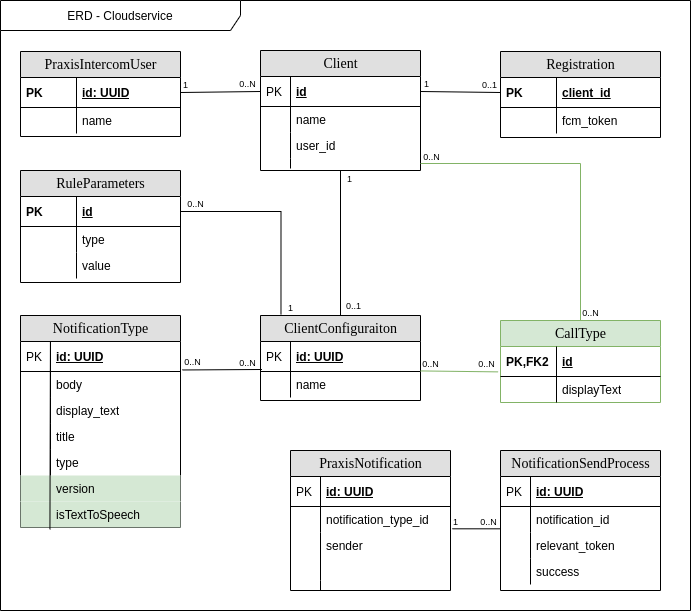
\includegraphics[width=\textwidth]{graphics/diagramms/erd_v02}}
        \caption{Entitiy Relation Diagramm - Cloudservice}
    \end{minipage}
\end{figure}

\clearpage

\subsection{Native iOS Applikation}

Dieses Kapitel beschreibt das Konzept für einen nativen iOS Client zur Bedienung von Praxisruf.
Es wird Entwurf und Funktionsweise der notwendigen Ansichten der Benutzeroberfläche beschrieben.
Weiter wird definiert, wie die aus dem Vorgängerprojekt zu migrierenden Funktionen in eine native iOS Applikation integriert werden können.
Dies beinhaltet insbesondere Anbindung der API des Cloudservice und Firebase Cloud Messaging.
Die Integration von Gegensprechanlage und Sprachsynthese wird nur im Rahmen des Entwurfs der Benutzeroberfläche beschrieben.
Eine detaillierte Beschreibung der Konzepte für diese Features folgt in den Kapiteln 7.3 und 7.4.


\subsubsection{Benutzeroberfläche}

Die Ansichten zur Anmeldung und Zimmerauswahl werden analog zum bestehenden Mobile Client umgesetzt.
Die Loginseite beinhaltet einen kurzen Willkommenstext und ein Logo für Praxisruf.
Darunter findet sich ein einfaches Formular zur Eingabe von Benutzername und Passwort, sowie ein Button zur Bestätigung.

\begin{figure}[h]
    \centering
    \begin{minipage}[b]{0.4\textwidth}
        \fbox{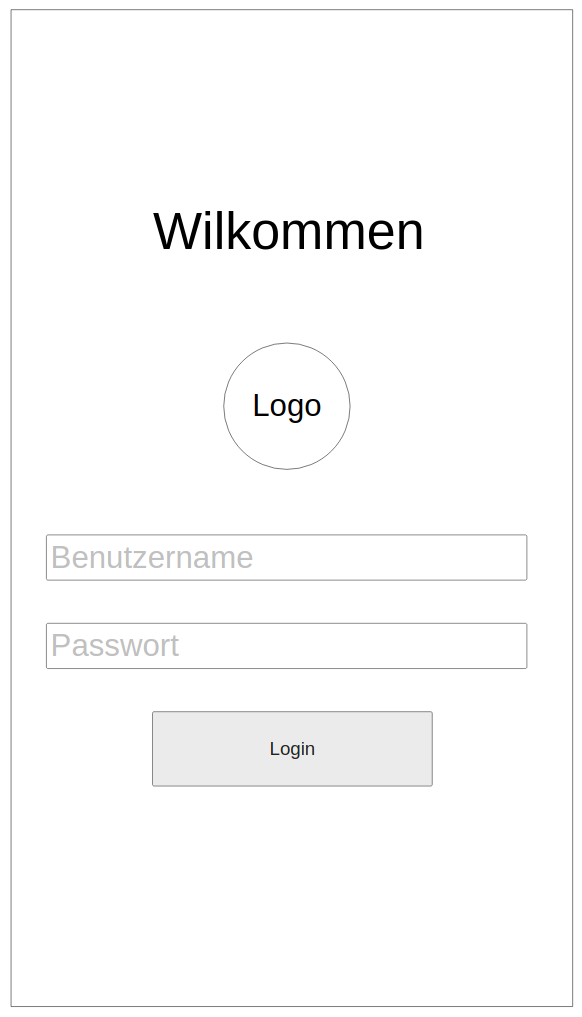
\includegraphics[width=\textwidth]{/home/joshua/FHNW/dev/IP6/IP6_Bachelorarbeit_Bericht_Cloudbasiertes_Praxisrufsystem/src/graphics/mockups/mockup_login}}
        \caption{Mockup Login}
    \end{minipage}
    \hfill
    \begin{minipage}[b]{0.4\textwidth}
        \fbox{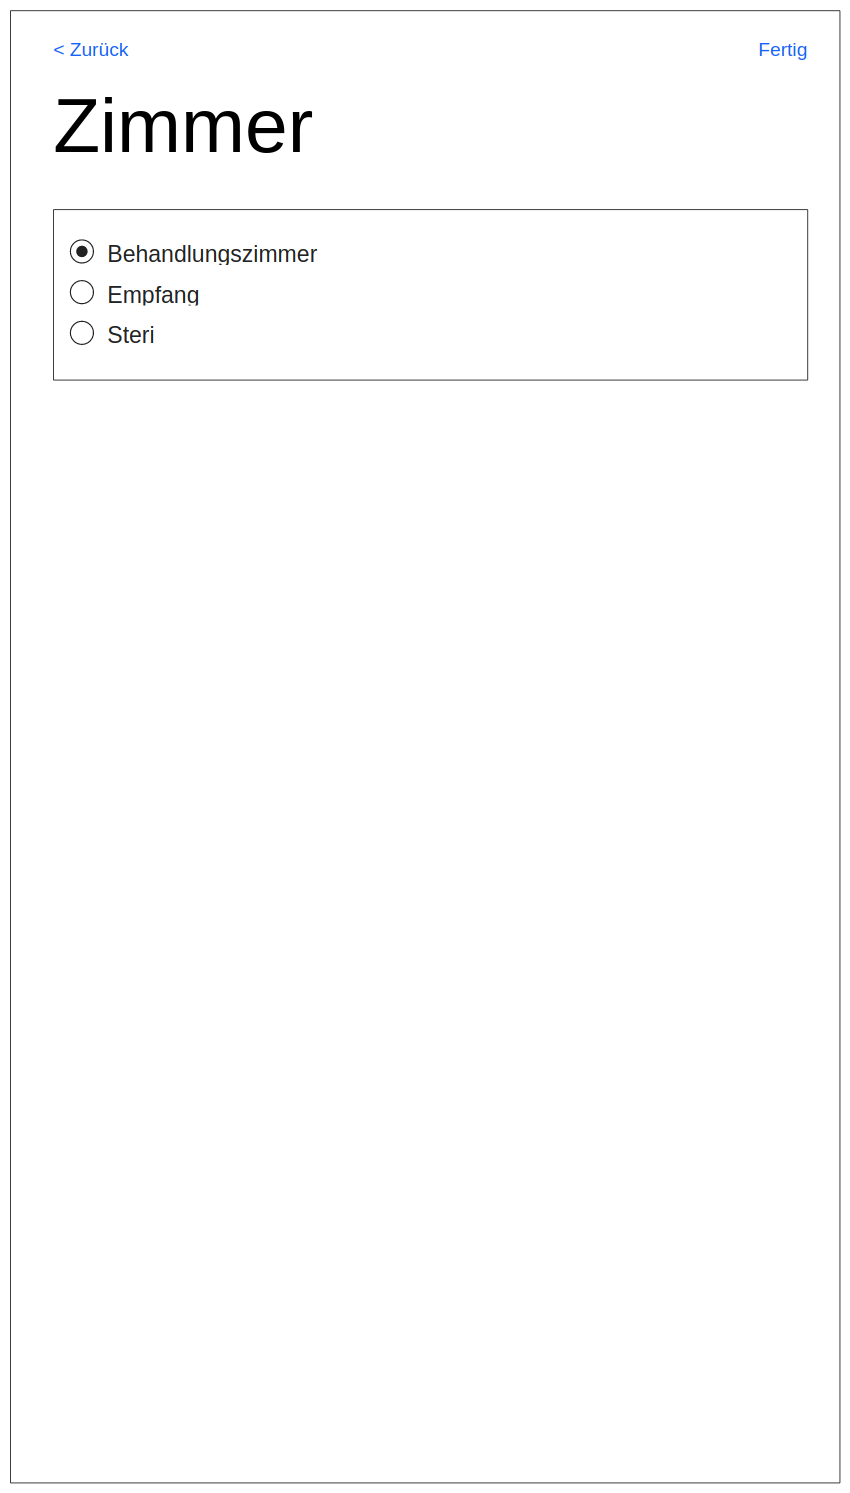
\includegraphics[width=\textwidth]{/home/joshua/FHNW/dev/IP6/IP6_Bachelorarbeit_Bericht_Cloudbasiertes_Praxisrufsystem/src/graphics/mockups/mockup_clientselect}}
        \caption{Mockup Zimmerwahl}
    \end{minipage}\label{fig:Mockups-Login-ClientSelection}
\end{figure}

Nach dem Eingeben der Anmeldedaten werden Praxismitarbeitende aufgefordert, die gewünschte Konfiguration auszuwählen.
Die Ansicht besteht aus einem Seitentitel und einer Liste zur Auswahl der gewünschten Konfiguration.
In der Auswahl sind alle Zimmer zu sehen, welche dem Benutzer zur Verfügung stehen.
Diese Konfigurationen müssen vor der Anmeldung im Admin UI erfasst und dem Benutzer zugewiesen werden.
In der Kopfzeile sind die Schaltflächen ''Zurück'' und ''Fertig'' zu sehen.
Die Schaltfläche ''Zurück'', bricht die Anmeldung ab und führt zurück zur Eingabe der Logindaten.
Die Schaltfläche ''Fertig'' bestätigt die Auswahl und leitet zur Hauptansicht weiter.
Wird bestätigt, ohne dass ein Zimmer angewählt ist, wird dem Benutzer eine Fehlermeldung angezeigt und nicht zur Hauptansicht weitergeleitet.

Die Hauptansicht der Applikation gliedert sich in die Bereiche Home, Inbox und Einstellungen.
Zwischen den drei Bereichen kann über eine Leiste am unteren Ende des Bildschirms navigiert werden.
Die Ansicht Home zeigt dem Benutzer die Buttons, über welche er Benachrichtigungen versenden und Anrufe in der Gegensprechanlage starten kann.
Wird ein Anruf gestartet, wird die Ansicht für aktive Anrufe angezeigt.
Diese zeigt dem Benutzer den Titel des gestarteten Anrufs, sowie eine Liste aller Teilnehmer zusammen mit dem Verbindungsstatus jedes Teilnehmers.
Der Titel des Anrufes entspricht dem Anzeigetext des verwendeten Buttons für ausgehende Anrufe und dem Namen des Anrufers für empfangene Anrufe.
Neben den Anrufinformationen zeigt die Ansicht für aktive Anrufe drei Buttons.
Über diese können Mikrofon und Lautsprecher des eigenen Gerätes stumm geschaltet werden.
Weiter kann der Anruf über einen roten Button am rechten Rand beendet werden.
Nach einem beendeten Anruf wird automatisch zu der zuvor angezeigten Ansicht navigiert.

\begin{figure}[h]
    \centering
    \begin{minipage}[b]{0.4\textwidth}
        \fbox{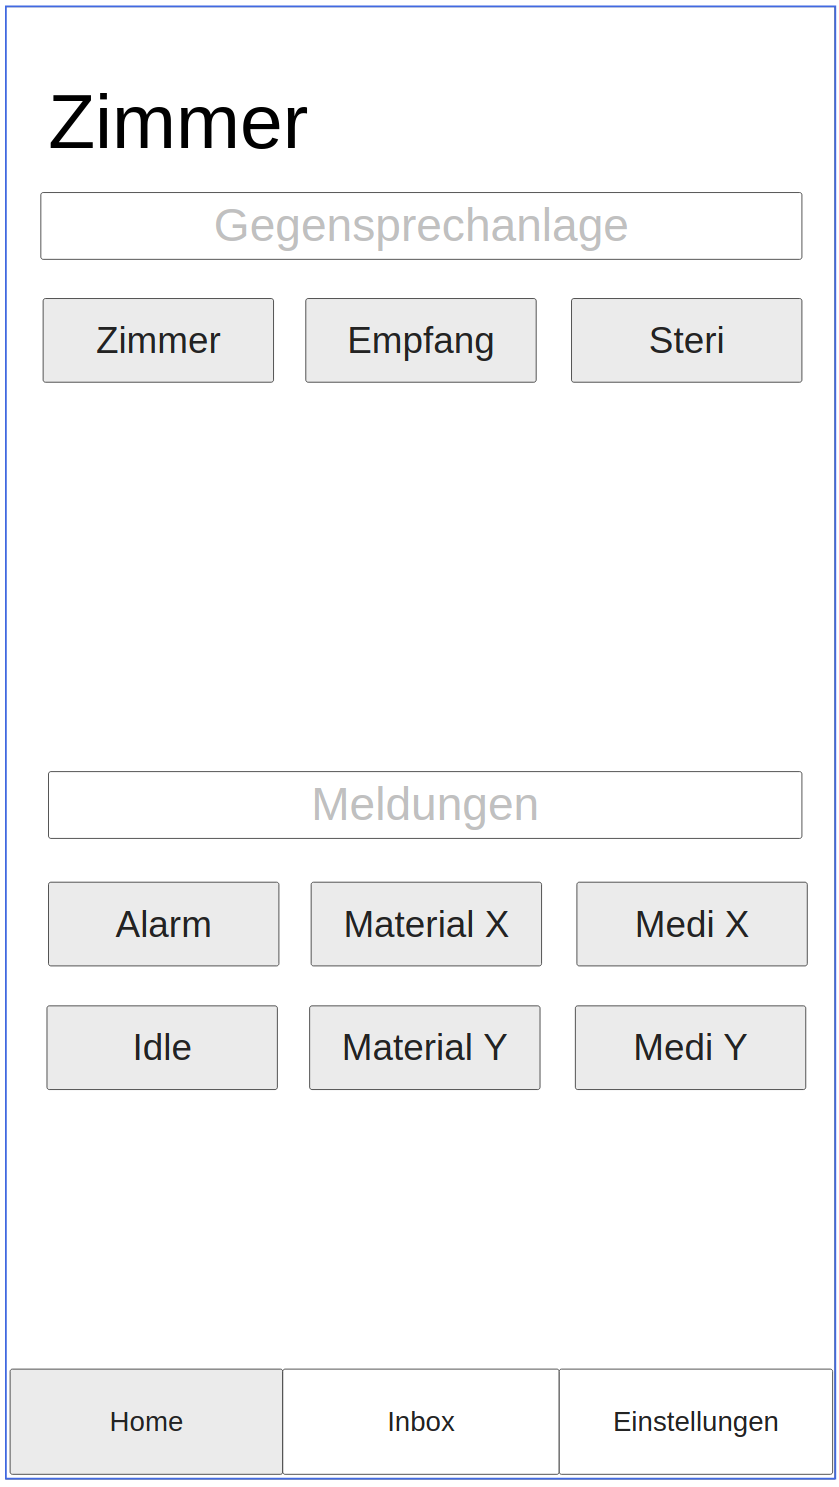
\includegraphics[width=\textwidth]{/home/joshua/FHNW/dev/IP6/IP6_Bachelorarbeit_Bericht_Cloudbasiertes_Praxisrufsystem/src/graphics/mockups/mockup_intercom}}
        \caption{Mockup Home}
    \end{minipage}
    \hfill
    \begin{minipage}[b]{0.4\textwidth}
        \fbox{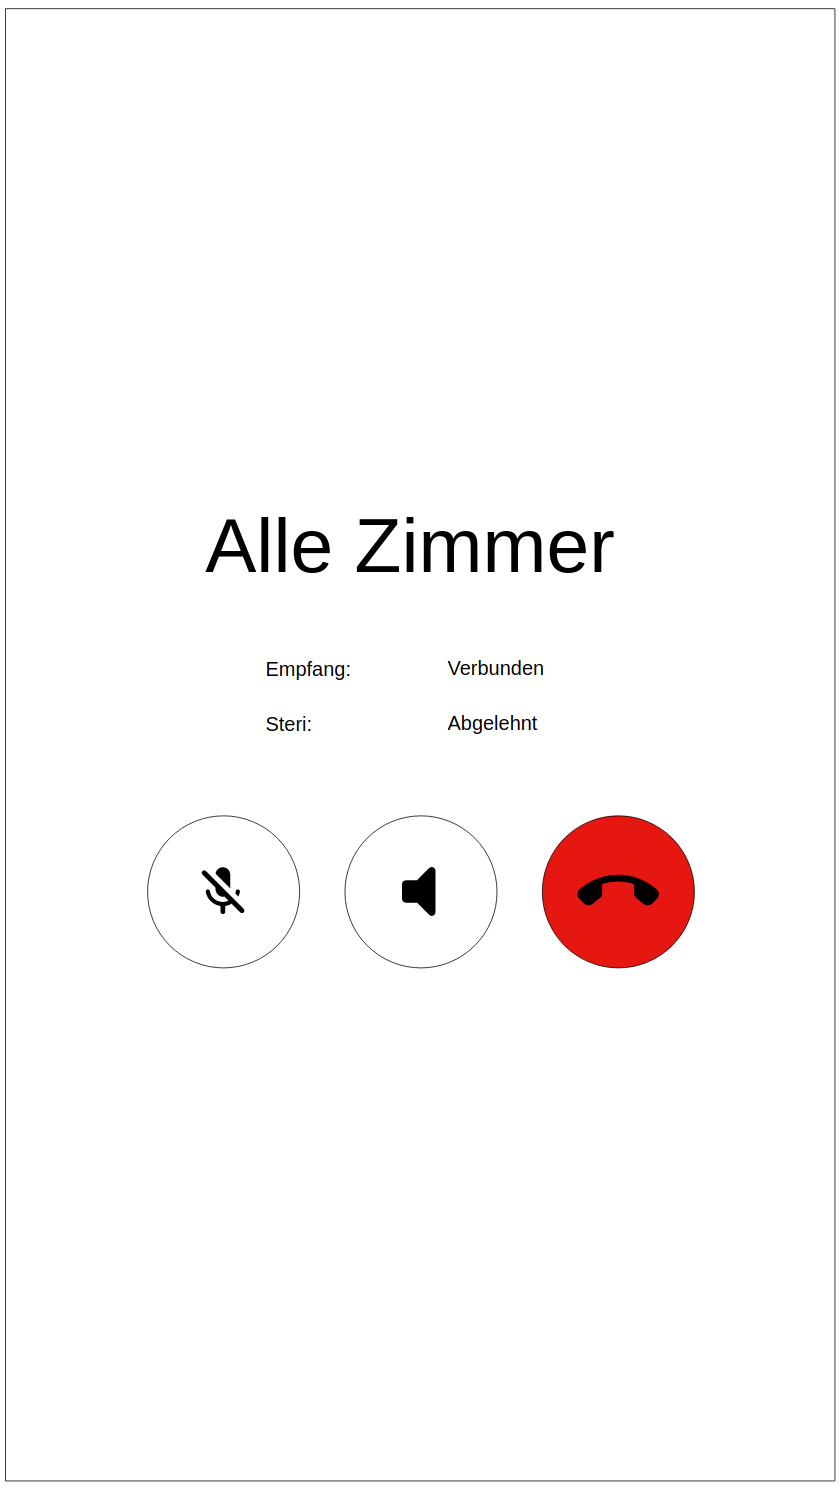
\includegraphics[width=\textwidth]{/home/joshua/FHNW/dev/IP6/IP6_Bachelorarbeit_Bericht_Cloudbasiertes_Praxisrufsystem/src/graphics/mockups/mockup_call}}
        \caption{Mockup Aktiver Anruf}
    \end{minipage}\label{fig:Mockups-Home-ActiveCall}
\end{figure}

Der Bereich Inbox zeigt eine Liste der empfangenen Benachrichtigungen sowie der empfangenen und verpassten Anrufe.
Für alle Elemente in der Inbox wird der Name des Senders als Überschrift angezeigt.
Darunter werden weitere Detailinformationen beschrieben.
Für Benachrichtigungen beinhaltet dies den Textinhalt der Benachrichtigungen.
Bei Anrufen beschrieben ob, es sich um einen empfangenen, verpassten oder abgelehnten Anruf handelt.
Einträge für Benachrichtigungen sowie verpasste und abgelehnte Anrufe müssen durch eine Wischgeste quittiert werden.
Die Funktionsweise der Quittierung wird aus dem bestehenden Mobile Client übernommen.
Quittierte Meldungen werden aus der Inbox entfernt und nicht mehr angezeigt.
Ein Quittieren von Meldungen und Anrufen passiert ausschliesslich lokal in der iOS Applikation.
Der Empfänger wird nicht über die Quittierung informiert~\cite{ip5}.

Es muss sichergestellt werden, dass verpasste Benachrichtigungen und Anrufe nicht übersehen werden.
Dazu wird im Abstand von 60 Sekunden geprüft, ob unquittierte Benachrichtigungen oder Anrufe in der Inbox vorhanden sind.
Ist dies der Fall, wird ein Erinnerungston abgespielt und eine Benachrichtigung angezeigt.
Dieser Mechanismus wird in Kapitel 7.2.4 weiter beschrieben.

\begin{figure}[h]
    \centering
    \begin{minipage}[b]{0.4\textwidth}
        \fbox{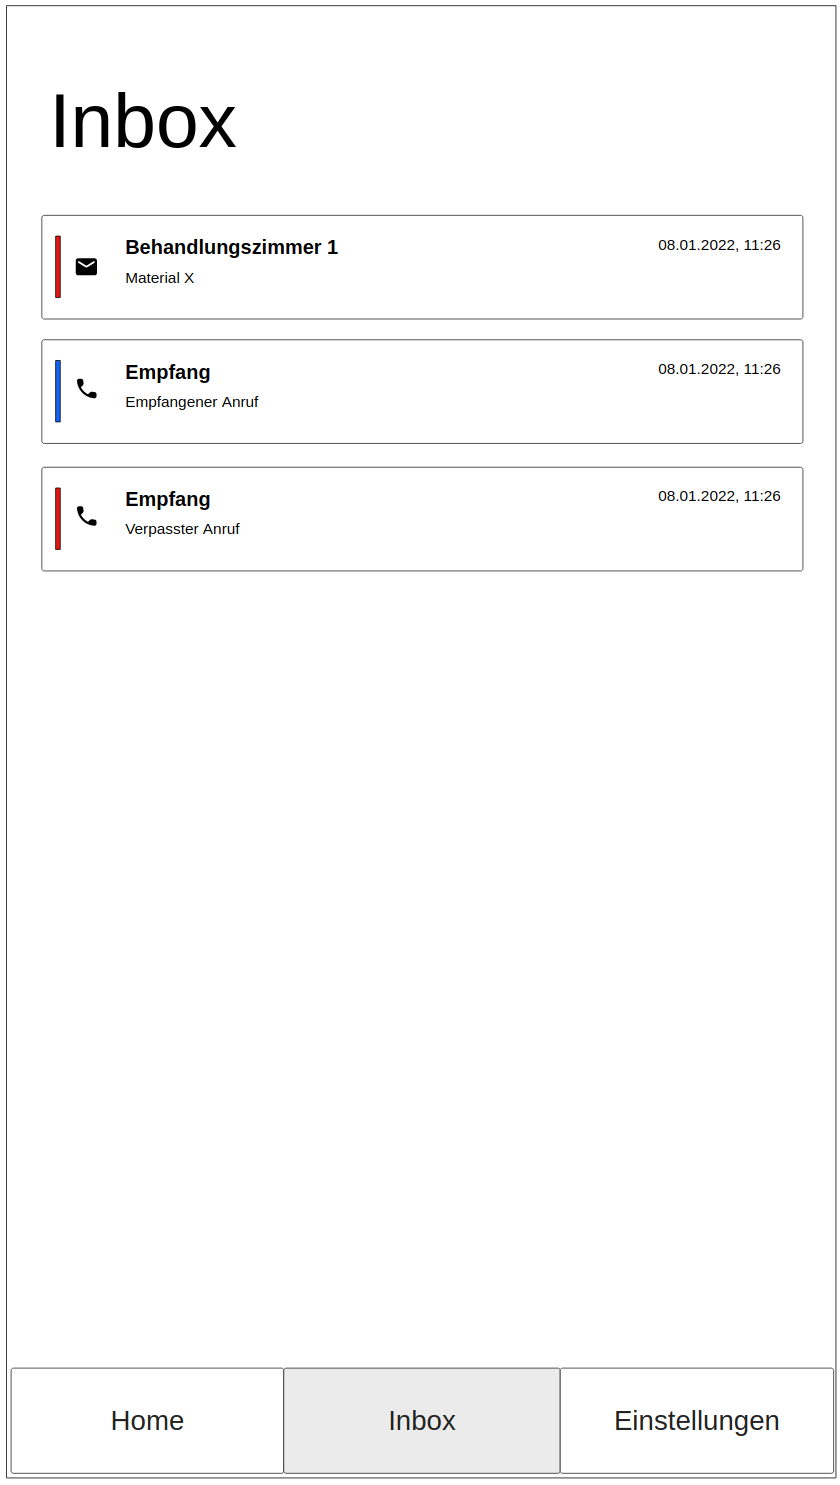
\includegraphics[width=\textwidth]{/home/joshua/FHNW/dev/IP6/IP6_Bachelorarbeit_Bericht_Cloudbasiertes_Praxisrufsystem/src/graphics/mockups/mockup_inbox}}
        \caption{Mockup Inbox}
    \end{minipage}
    \hfill
    \begin{minipage}[b]{0.4\textwidth}
        \fbox{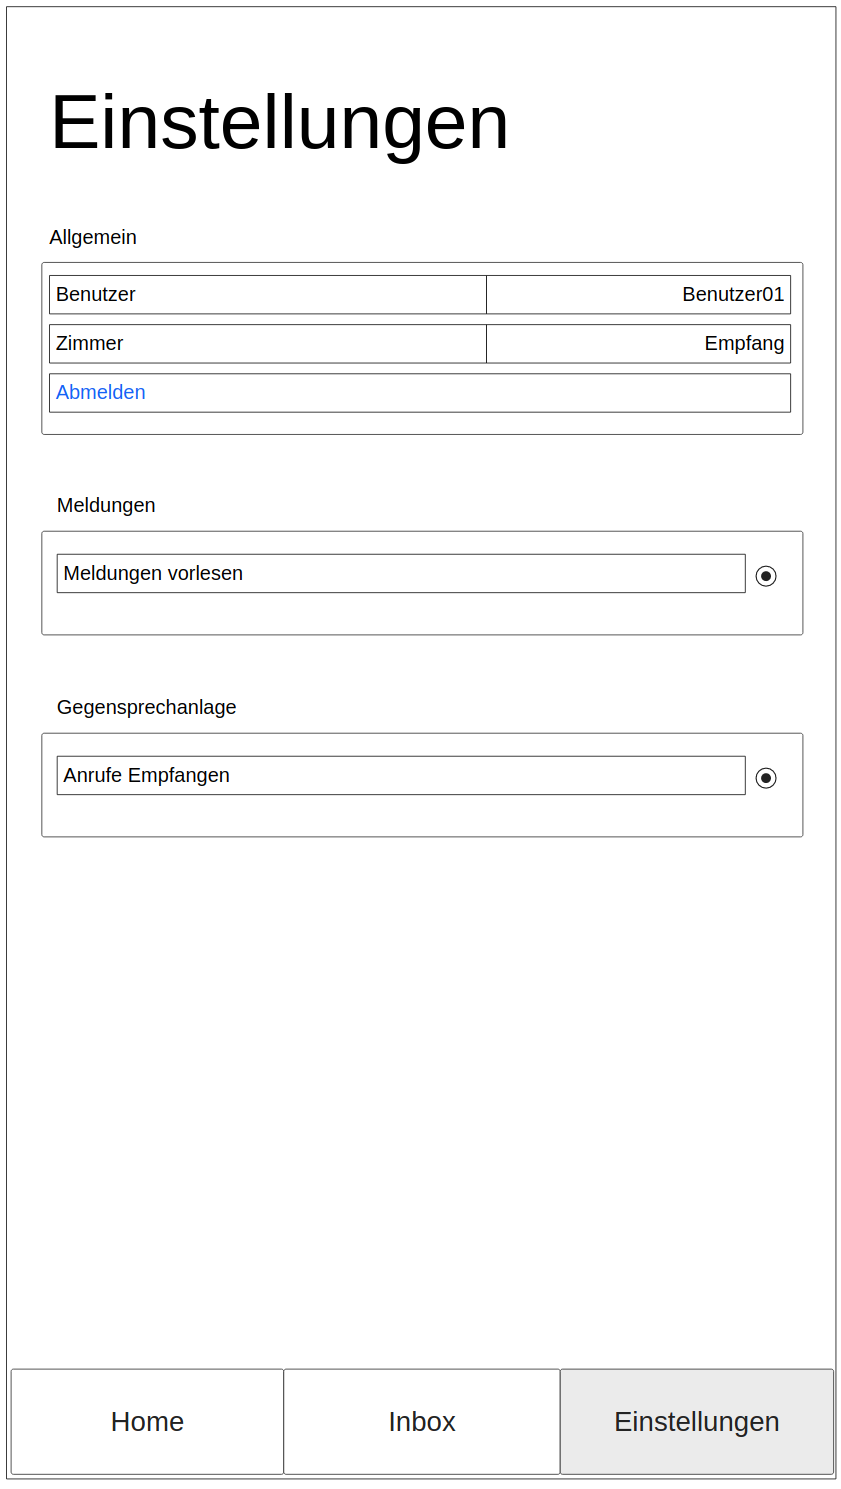
\includegraphics[width=\textwidth]{/home/joshua/FHNW/dev/IP6/IP6_Bachelorarbeit_Bericht_Cloudbasiertes_Praxisrufsystem/src/graphics/mockups/mockup_settings}}
        \caption{Mockup Einstellungen}
    \end{minipage}\label{fig:Mockups-Inbox-Settings}
\end{figure}

Abbildung 7.8 zeigt den Bereich Einstellungen.
Der Bereich Einstellungen zeigt den aktuellen Benutzernamen und die gewählte Konfiguration.
Über die Schaltfläche Abmelden, können sich Praxismitarbeitende aus der Applikation abmelden.
Die Schaltfläche Benachrichtigungen vorlesen ist standardmässig aktiviert.
Wird die Option deaktiviert, werden Benachrichtigungen nie vorgelesen.
Die Schaltfläche Anrufe empfangen ist ebenfalls standardmässig aktiviert.
Wird diese Option deaktiviert, werden alle empfangenen Anrufe automatisch abgelehnt und stattdessen eine Benachrichtigung angezeigt.
Ausgehende Anrufe können auch getätigt werden, wenn diese Option aktiviert ist.

\subsubsection{Anbindung Cloudservice API}

Der Mobile Client muss an die API des Cloudservices angebunden werden.
Es wird eine Anbindung an die Domäne Configuration zur Anmeldung und Auswahl des gewünschten Zimmers und an die Domäne Notification zum Versenden von Benachrichtigungen benötigt.
Die Schnittstellen dieser Domänen stehen als Http Endpunkte zur Verfügung.
In diesem Unterkapitel wird beschrieben, wie Http-Anfragen an die Cloudservice API in den nativen iOS Client integriert werden.
Das Abrufen von Sprachdaten und die Anbindung an die Signaling Instanz werden in den Kapiteln 7.3 und 7.4 beschrieben.

Die Basisbibliothek für iOS Entwicklung bietet die Klasse URLSession, über welche Netzwerkaufrufe getätigt werden können.
Über URLSession.shared steht eine Standard-Instanz zur Verfügung, über welche Netzwerkanfragen verarbeitet werden können~\cite{ios_urlsession}.
Die Klasse UrlRequest ermöglicht es, Http-Request für eine URL mit Header und Body zu erstellen~\cite{ios_urlrequest}.
Um die Integration dieser Klassen in die Applikation zu vereinfachen, wird ein zentraler Service mit dem Namen PraxisrufApi erstellt.
Dieser kapselt das Erstellen, Befüllen und Absetzten der nötigen UrlRequest Instanzen.
Er bietet öffentliche Methoden für die Http Verben Get, Post und Delete an.
Über diese können Http-Requests mit der jeweiligen Methode abgesetzt werden.
Zur Darstellung von Fehlern wird die Enum PraxisrufApiError erstellt.
Diese definiert Fehlerkategorien und wird von PraxisrufApi verwendet, um Aufrufern das Fehlschlagen einer Anfrage mitzuteilen.
Das Klassendiagramm in Abbildung 7.9 zeigt den Aufbau des Service PraxisrufApi\@.

\begin{figure}[h]
    \centering
    \begin{minipage}[b]{0.8\textwidth}
        \fbox{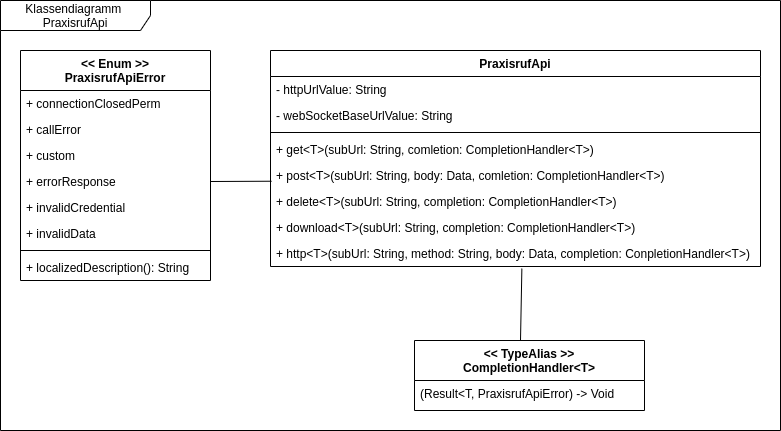
\includegraphics[width=\textwidth]{graphics/diagramms/Class_PraxisrufAPI}}
        \caption{Klassendiagramm PraxisrufApi}
    \end{minipage}
\end{figure}

Die Basis-URL für Http-Anfragen wird in der Konfiguration der iOS Applikation definiert.
Der PraxisrufApi Service lädt diese und verwendet sie für alle Abfragen, die abgesetzt werden.
Alle öffentlichen Methoden von PraxisrufApi nehmen einen Parameter ''subUrl'' als String entgegen.
Dieser String wird der Basis-URL angehängt.
Die Methoden Post nimmt zudem einen optionalen Parameter von Typ Data entgegen.
Dieser definiert den Inhalt des Request Bodies.
Mit diesen Informationen kann der Http Request erstellt und versendet werden.

Sämtliche öffentlichen Methoden des PraxisrufApi Service nehmen weiter einen Parameter mit dem Namen completion entgegen.
Dabei handelt es sich um eine Funktion, welche beim Erfolg oder Fehlschlagen der Http-Anfragen ausgeführt wird.
Als Parameter dieser Funktion wird immer der Typ Result$<$T, PraxisrufApiError$>$ verwendet.
Bei Result handelt es sich um einen Wrapper Typen welcher entweder das Resultat einer Abfrage oder ein Fehlerobjekt beinhaltet~\cite{ios_result}.
Im Fehlerfall wird das Result mit einem PraxisrufApiError Objekt erstellt.
Im Erfolgsfall wird es mit den Daten aus dem Body der Http-Antwort befüllt.
Zur Darstellung dieser Daten wird der generische Typ T verwendet.
Der Typ wird vom Aufrufer von PraxisrufApi definiert und kann grundsätzlich beliebig sein.
Er muss aber das Protokoll Decodable aus der iOS Standardbibliothek implementieren.
Decodable Instanzen können von einer JSON-String-Repräsentation in ein Swift-Objekt konvertiert werden~\cite{ios_decodable}.
So kann das Resultat im Erfolgsfall aus der Response generiert und an, dass Callback übergeben werden.
Dadurch kann die Konvertierung generisch in im PraxisurfApi-Service behandelt werden.

Anhand des Inhalts der Result-Instanz kann geprüft werden, ob die Anfrage erfolgreich war.
Das Resultat kann entsprechend verarbeitet werden.
Diese Prüfung und Verarbeitung findet innerhalb der completion-Funktion statt.
Dieser Ansatz ermöglicht es im PraxisrufApi-Service ausschliesslich Http-Anfragen zu senden und die entsprechenden Antworten entgegenzunehmen.
Der Api Service behandelt damit ausschliesslich die technische Anbindung an die API des Cloudservice.
Er muss keine fachliche Logik implementieren und kann generisch für alle Anwendungen wiederverwendet werden.

Requests die über den PraxisrufApi-Service erstellt werden, werden automatisch authentisiert.
Dazu lädt der Service die hinterlegten Credentials aus dem KeyStore von iOS.
Das Token wird verwendet, um einen entsprechenden Authorization-Header zu generieren.
Der generierte Authorization Header wird der Http-Anfrage angefügt.
Ist kein Token vorhanden, wird keine Anfrage abgesetzt.
Es wird direkt die completion-Funktion mit dem Fehler PraxisrufApiError.invalidCredential aufgerufen.

Mit dieser Lösung steht ein Service zur Verfügung, über welchen Http-Anfragen einfach in eine iOS App integriert werden können.
Dank der generischen Methoden im PraxisrufApi-Service können neue Calls einfach hinzugefügt werden, ohne das Boilerplate-Code wiederholt werden muss.
Durch die completion-Funktionen kann die fachliche Verarbeitung von Http-Anfragen vom Aufrufer definiert werden.

Um die Verwendung der Cloudservice API weiter zu vereinfachen, wird der PraxisrufApi Service um sprechende Methoden für die nötigen Abfragen erweitert.
Dazu wird pro Domäne eine Extension-Klasse erstellt.
Diese fügt Methoden mit sprechenden Namen für die angesprochene Funktionalität hinzu und kapseln die Verwendung der Get, Post und Delete Methoden.

Der PraxisrufApi-Service ermöglicht es Abfragen an die Cloudservice API abzusetzen.
Die Resultate dieser Abfragen müssen in der Benutzeroberfläche angezeigt werden können.
Es wird pro Domäne ein weiterer Service geschrieben, welche den Aufruf des API Services kapselt.
Dieser Service bietet Methoden, über welche der PraxisrufApi Service angesprochen werden kann.
View-Komponenten können diese Services nutzen, um durch Benutzereingaben ausgelöste Anfragen an die Cloudservice Api zu senden.
Resultate und Fehler aus Anfragen an den Cloudservice werden in diesen Services als Instanzvariablen gehalten.
Die View-Komponenten können lesend auf diese Variablen zugreifen, um die entsprechenden Resultate oder Fehler anzuzeigen.

\subsubsection{Anbindung Messaging Service}

Um Benachrichtigungen empfangen zu können, muss Firebase Cloud Messaging an die native iOS Applikation angebunden werden.
Firebase bietet eine Bibliothek mit welcher Firebase Cloud Messaging in iOS Clients integriert werden kann~\cite{firebase_ios}.
Diese Integration kann allerdings nicht mit dem Mitteln von SwiftUI implementiert werden.
Dies liegt daran, dass für das Empfangen von Benachrichtigungen und das Anzeigen von Push-Benachrichtigungen Integration mit dem Benachrichtigungszenter des Betriebssystem notwendig ist.
Diese Integration kann bis heute nur über AppDelegates umgesetzt werden.
SwiftUI Applikationen können oft ohne AppDelegates implementiert werden.
Sobald aber Integration mit dem Betriebssystem notwendig ist, müssen AppDelegates verwendet werden.
Dazu können AppDelegates bei der Initialisierung der Applikation registriert werden.

Zur Anbindung von Firebase Cloud Messaging wird dementsprechend ein AppDelegate implementiert.
Die Logik des Delegates wird dabei auf das minimal Nötige reduziert.
Der AppDelegate selbst ist für die direkte Kommunikation mit Firebase verantwortlich und muss empfangene Daten an Betriebssystem und SwiftUI Applikation übergeben.
Fachliche Logik wird nicht im AppDelegate, sondern in der SwiftUI Applikation ausgeführt.
Dies ermöglicht es die Anbindung des Messaging Service im AppDelegate zu kapseln.
Sollte Firebase Cloud Messaging in Zukunft durch einen anderen Anbieter ersetzt werden, muss damit ausschliesslich die Logik im AppDelegate angepasst werden.
Diese Trennung stellt sicher, dass die Fachlogik vollständig mit SwiftUI implementiert werden kann.
Der AppDelegate beinhaltet lediglich die Teile, welche aus technischen Gründen nicht mit SwiftUI umgesetzt werden können.

Um Benachrichtigungen von Firebase Cloud Messaging empfangen zu können, muss der AppDelegate folgende Funktionalität umsetzen.
Beim Start der Applikation muss sich der Mobile Client beim Messaging Service registrieren.
Nach der Registrierung wird für den Mobile Client ein Token generiert, welches den Client eindeutig beim Messaging Service identifiziert.
Der AppDelegate muss, darauf reagieren und das erneuerte Token an die Applikation übergeben.

Für die Verarbeitung von Benachrichtigungen muss der AppDelegate Benachrichtigungen im Vordergrund empfangen und dem Betriebssystem zur Anzeige übergeben.
Die Informationen aus der empfangenen Benachrichtigung müssen anschliessend an die Applikation übergeben werden.
Benachrichtigungen, die im Hintergrund empfangen werden, müssen an das Betriebssystem übergeben und angezeigt werden.
Sobald die Applikation wieder in den Vordergrund tritt, müssen die Daten an die Applikation zur weiteren Verarbeitung übergeben werden.

\subsubsection{Benachrichtigungen prüfen}

Der bestehende Mobile Client prüft in regelmässigen Abständen, ob ungelesene Benachrichtigungen in der Inbox vorhanden sind.
Wenn ungelesene Benachrichtigungen gefunden werden, wird ein Benachrichtigungston abgespielt.
Im Mobile Client der Vorgängerlösung findet diese Prüfung nur statt, wenn die Applikation in Vordergrund aktiv ist.
Diese Funktion wird in der nativen iOS Applikation übernommen.

Für die Umsetzung der Erinnerungsfunktion werden zwei Services definiert.
Erstens wird eine Inbox erstellt, welche eine Liste der aktuellen Benachrichtigungen führt.
Zweitens wird ein InboxReminderService implementiert.
Dieser prüft den Inhalt der Inbox und sucht nach unquittierten Elementen, welche älter als eine Minute sind.
Werden solche Elemente gefunden, wird eine Benachrichtigung angezeigt und ein Benachrichtigungston abgespielt.
Die regelmässige Prüfung der Inbox wird mit der Timer-Klasse der iOS Standardbibliothek umgesetzt.
Über diese ist es möglich auf einer View in regelmässigen Abständen Events auszulösen~\cite{ios_timer}.
Ein solcher Timer wird auf der Hauptansicht für angemeldete Benutzer registriert.
Der Timer löst alle 60 Sekunden die Prüfung des InboxReminderService aus.

Die Prüfung von Benachrichtigungen im Hintergrund wird im Rahmen dieses Projektes nicht umgesetzt.
Für künftige Erweiterungen ist es möglich diese Funktion zu implementieren.
Um dies zu ermöglichen, müssen Benachrichtigungen auf dem Gerät persistiert werden.
So stehen die Daten auch zur Verfügung, wenn die Applikation nicht gestartet ist.
Weiter muss ein Hintergrundtask implementiert und registriert werden~\cite{ios_bgtaskscheduler}, welcher die persistierten Daten lädt und die darauf die Prüfung des InboxReminderService ausführt.

\subsubsection{Security}

In einem Praxisrufsystem muss die sichere Übertragung von Daten gewährleistet sein.
Die dazu definierten Konzepte werden aus dem Vorgängerprojekt übernommen.

Alle Daten zwischen den Services müssen über verschlüsselte Verbindungen ausgetauscht werden.
HTTP Anfragen CloudService API erfolgen ausschliesslich über HTTPS\@.
Alle Anfragen an die API des Cloudservice müssen zudem mit einem Json Web Token (JWT) authentifiziert sein.
Praxismitarbeitende werden durch den Cloudservice mittels Basic Authentication authentifiziert.
Bei der Anmeldung mit Benutzername und Passwort liefert der Cloudservice ein JWT, welches vom Client für weitere Anfragen verwendet wird.
Sowohl die Credentials für die Basic Authentication als auch das JWT Token werden durch die iOS Applikation im Keystore des Betriebssystems gespeichert~\cite{ip5}.
Das Token wird regelmässig erneuert, indem die Basic Authentication mit den gespeicherten Credentials wiederholt wird.
Der Ablauf für Authentifizierung wird damit unverändert aus dem Vorgängerprojekt übernommen.

\clearpage

\subsubsection{Servicemodell}

Dieses Kapitel gibt einen Überblick zu den Services welche in der nativen iOS Applikation beinhaltet werden.
Abbildung 7.10 zeigt das vollständige Modell der implementierten Services.
Diese Darstellung beinhaltet die Services, welche in den Kapiteln 7.2 bis 7.4 beschrieben werden.
View- und Model-Komponenten werden hier nicht dargestellt.

\begin{figure}[h]
    \centering
    \begin{minipage}[b]{1\textwidth}
        \fbox{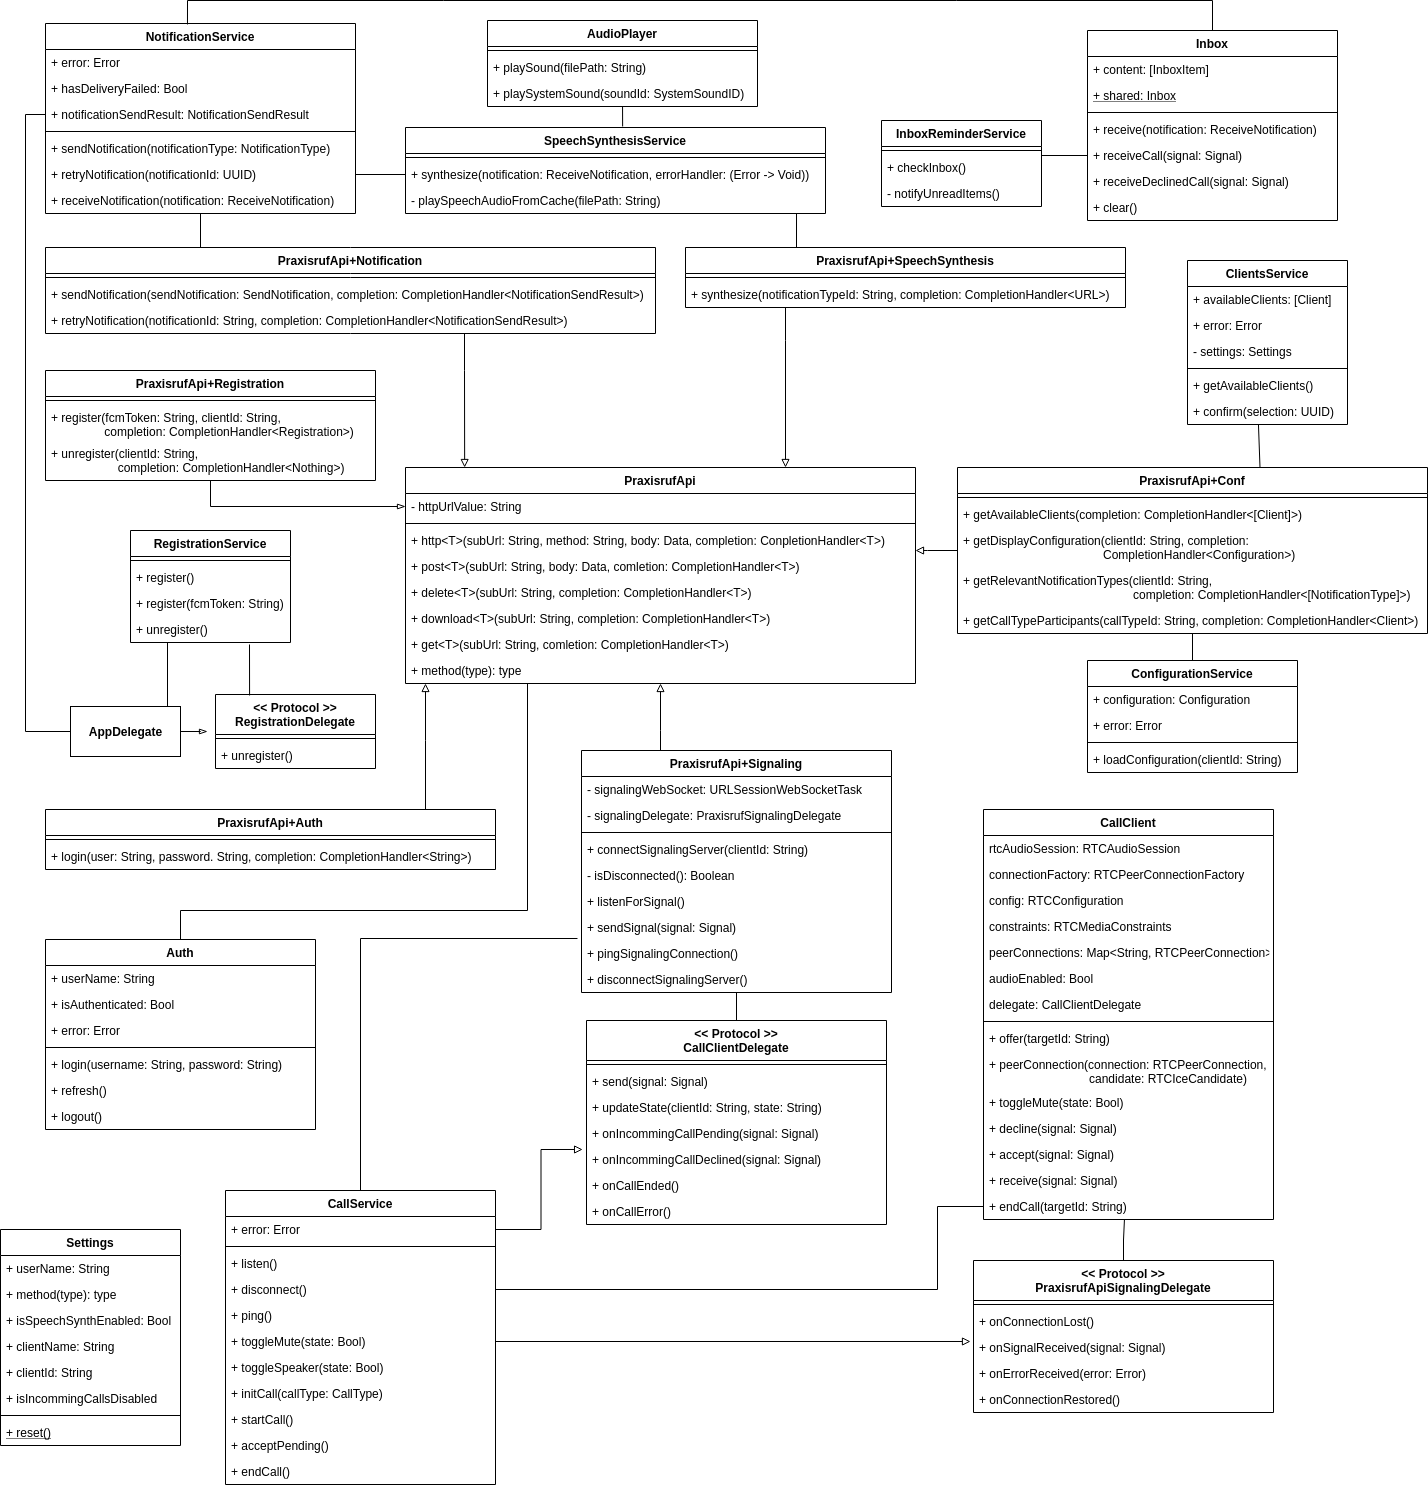
\includegraphics[width=\textwidth]{/home/joshua/FHNW/dev/IP6/IP6_Bachelorarbeit_Bericht_Cloudbasiertes_Praxisrufsystem/src/graphics/diagramms/Class_Mobile_Client_Services}}
        \caption{Klassendiagramm - App Services}
    \end{minipage}
\end{figure}

Die Klasse Settings wird verwendet um die Konfiguration des Benutzers zu verwalten.
Sie bietet Getter und Setter für alle Properties.
Nach dem setzten eines Wertes, wird dieser über die Komponente UserData aus der iOS Standardbibliothek persistiert.
Die Verwendungen der Settings-Klasse sind in Abbildung 7.10 nicht dargestellt, um die Übersichtlichkeit zu wahren.

\clearpage

\subsection{Sprachsynthese}

Dieses Kapitel beschreibt die Integration von Sprachsynthese in Praxisruf.
Der Fokus liegt dabei auf den Abläufen zum Empfangen von Benachrichtigungen und dem Abrufen der Sprachdaten.
Der Empfang von Benachrichtigungen wird so erweitert, dass der Inhalt empfangener Benachrichtigungen automatisch vorgelesen wird.

\subsubsection{Konfiguration}

Benachrichtigungen für Praxisruf können über das Admin UI konfiguriert werden.
Es können pro Benachrichtigung Titel, Inhalt, Beschreibung sowie ein Anzeigetext erfasst werden.
Der Anzeigetext wird als Text des Buttons verwendet, über welchen die Benachrichtigung versendet wird.
Diese Konfiguration wird über die Entität NotificationType verwaltet.
Neu soll auch konfiguriert werden können, ob eine Benachrichtigung für die Sprachsynthese relevant ist.
Dazu wird die Entität NotificationType um ein boolean Flag mit dem Namen ''isTextToSpeech'' erweitert.
Dieses Flag wird beim Versenden einer Benachrichtigung mitgesendet und kann vom Empfänger überprüft werden.
Wenn das Vorlesen von Benachrichtigungen in den lokalen Einstellungen und das Flag auf der Benachrichtigung aktiviert sind, wird die Benachrichtigungen vorgelesen.
Abbildung 7.11 zeigt einen Ausschnitt aus dem Entity Relationship Diagramm der Domäne Configuration.
Dabei sind die Felder, welche für die Sprachsynthese ergänzt werden, grün markiert.

\begin{figure}[h]
    \centering
    \begin{minipage}[b]{0.6\textwidth}
        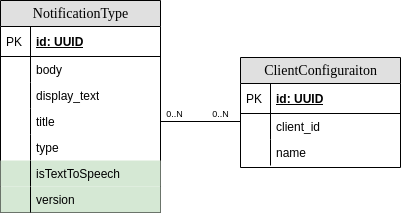
\includegraphics[width=\textwidth]{/home/joshua/FHNW/dev/IP6/IP6_Bachelorarbeit_Bericht_Cloudbasiertes_Praxisrufsystem/src/graphics/diagramms/erd_t2s_v01.drawio}
        \caption{ERD Ausschnitt - Konfiguration Sprachsynthese}
    \end{minipage}
\end{figure}

Neben dem Feld ''isTextToSpeech'', wird die NotificationType-Entität um ein weiteres Feld ''version'' erweitert.
Das Versionsfeld beinhaltet eine Ganzzahl, welche mit jeder Änderung inkrementiert wird.
Der Inhalt dieses Felds wird ebenfalls beim Versenden von Benachrichtigungen mitgesendet.
Auf Client-Seite wird diese Information zur Implementierung eines Cache verwendet.

\subsubsection{Anbindung von Sprachsynthese in Cloudservice}

Dieses Kapitel beschreibt, wie Amazon Polly an den Cloudservice angebunden wird, um das Vorlesen von Benachrichtigungen zu ermöglichen.

Die Anbindung an Amazon Polly erfolgt zentral im Cloudservice.
Sämtliche Anfragen an Amazon Polly werden durch den Cloudservice gemacht.
Empfänger von Benachrichtigungen senden keine direkten Anfragen an Amazon Polly.
Sie kommunizieren stattdessen mit dem Cloudservice.
Dieser führt die Anfrage an Amazon Polly aus und gibt die Resultate an den Anfrager zurück.

Für die Anbindung von Amazon Polly wird der Cloudservice um ein Modul mit dem Namen ''Speech Synthesis'' erweitert.
Dieses Modul muss unabhängig von allen anderen Domänen-Modulen des Cloudservice umgesetzt werden.
Werden Daten aus einer anderen Domäne benötigt, muss die Kommunikation über die API des entsprechenden Moduls gehen.
Diese Trennung ermöglicht es, das Modul in Zukunft einfach aus dem Cloudservice auszubauen und als eigenständigen Microservice zu betreiben.

Die Abhängigkeit zu Amazon Polly als Anbieter soll weitmöglichst minimiert werden.
So kann bei Bedarf einfacher auf einen anderen Provider gewechselt werden.
Um dies zu ermöglichen wird das Interface SpeechSynthesisService definiert.
Dieses gibt eine Methode vor, welche eine InputStreamResource zurückgibt.
Sie nimmt zwei Universal Unique Ids (UUID) als Parameter entgegennimmt.
Der erste Parameter entspricht der technischen Identifikation des zu synthetisierenden Benachrichtigungstypes (NotificationType).
Der zweite Parameter entspricht der Identifikation des Senders der Benachrichtigung.
Die InputStreamResource muss die synthetisierten Sprachdaten enthalten.
Dieses Interface wird von der Komponente, welche die Schnittstelle nach aussen bietet verwendet.
Um einen Anbieter für Sprachsynthese anzubinden, kann dieses Interface implementiert werden und der Schnittstelle zur Verfügung gestellt werden.
Das Klassendiagramm in Abbildung 7.12 gibt einen Überblick über den Aufbau des Moduls Speech Synthesis.

\begin{figure}[h]
    \centering
    \begin{minipage}[b]{1\textwidth}
        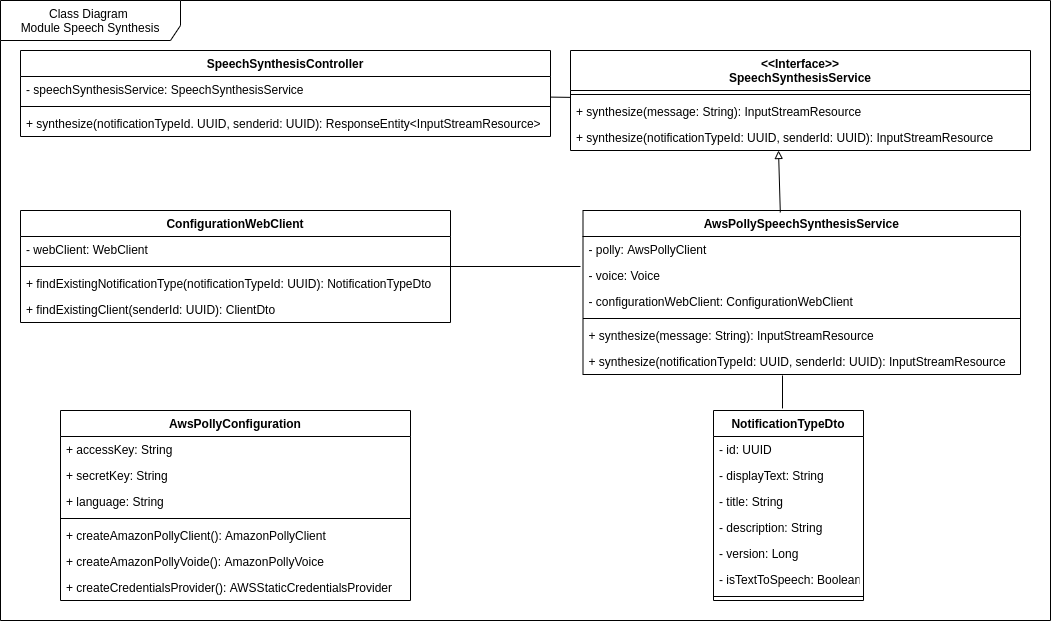
\includegraphics[width=\textwidth]{/home/joshua/FHNW/dev/IP6/IP6_Bachelorarbeit_Bericht_Cloudbasiertes_Praxisrufsystem/src/graphics/diagramms/Class_AWS_Polly_Configuration_V02}
        \caption{Klassendiagramm - Modul SpeechSynthesis}
    \end{minipage}
\end{figure}

Für die Anbindung des Providers Amazon Polly wird das Interface SpeechSynthesisService mit der Klasse AwsPollySpeechSynthesisService implementiert.
Amazon stellt einen Java Bibliothek für Amazon Polly zur Verfügung, welcher diese Anbindung ermöglicht~\cite{aws_polly_sdks}.
Diese Bibliothek bietet alle Klassen, die für die Anbindung an Amazon Polly nötig sind.
Sie wird bei in AwsPollySpeechSynthesisService verwendet, um Amazon Polly anzubinden.

Die Anbindung von Amazon Polly benötigt drei Komponenten.
Als Erstes muss eine Instanz von AWSStaticCredentialsProvider zur Verfügung gestellt werden.
Diese liefert die Credentials, welche das System berechtigen, Anfragen an Amazon Polly zu senden.
Als Zweites muss eine Voice konfiguriert werden.
Die Voice definiert Sprache und Stimme, welche für die Sprachausgabe verwendet wird.
Letztlich muss eine Instanz von AmazonPollyClient konfiguriert werden.
Dieser Client wird verwendet, um Anfragen an Amazon Polly zu senden.
Er verwendet den zuvor konfigurierten CredentialsProvider, um die Anfrage mit den entsprechenden Credentials zu ergänzen.
Die zuvor konfigurierte Voice wird bei Anfragen an Amazon Polly mitgesendet, damit die Daten mit den gewünschten Parametern synthetisiert werden.

Der Cloudservice ist als Java-Applikation mit Spring Boot umgesetzt.
Dies ermöglicht es, die notwendigen Komponenten in einer Spring Konfigurationsklasse zu konfigurieren und als Spring Beans zu instanziieren.
Über die Dependency Injection von Spring werden diese Komponenten dem AwsPollySpeechSynthesisService übergeben werden.

Werte, welche für die technische Konfiguration notwendig sind, werden aus der Konfigurationsdatei application.yml geladen.
Sprache und Region werden sich im Rahmen dieses Projektes nie ändern und beinhalten keine sensitiven Informationen.
Sie werden deshalb direkt in der Konfigurationsdatei definiert und mit dem Quellcode des Projektes verwaltet.
Als Credentials für die Anbindung dienen die zwei Schlüssel AccessKey und SecretKey.
Credentials werden nicht direkt in der Konfigurationsdatei gespeichert.
Stattdessen wird ein Platzhalter definiert, welcher die Werte für Credentials aus entsprechend benannten Umgebungsvariablen lädt.
Die Zugangsdaten müssen damit nicht mit dem Quellcode verwaltet werden.

\subsubsection{Sprachsynthese über Cloudservice API}

Endgeräte in Praxisruf müssen Sprachdaten über den Cloudservice beziehen können.
Das Modul Speech Synthesis stellt deshalb eine Schnittstelle zur Verfügung, über welche Sprachdaten abgefragt werden können.
Dabei ist es nicht möglich beliebige Textdaten in Sprachdaten zu verwandeln.
Stattdessen erlaubt die Schnittstelle die Abfrage von Sprachdaten für Inhalt und Sender einer Benachrichtigung.

Als Inhalt einer Benachrichtigung wird das Feld ''title'' aus der Entität NotificationType verwendet.
Der Name des Senders wird dem Feld ''name'' der Entität Client entnommen.
Beide Entitäten sind Teil des Moduls Configuration.
Die entsprechenden Daten müssen deshalb über die API des Configuration-Moduls geladen werden.
Um dies zu ermöglichen, werden die Identifikatoren der relevanten Entitäten zusammen mit Benachrichtigung versendet.

Der Endpunkt zum Bezug von Sprachdaten nimmt die zwei Parameter ''notificationTypeId'' und ''sender'' entgegen.
Diese müssen die technischen Identifikatoren der jeweiligen Entitäten beinhalten.
Anhand dieser Parameter werden der die benötigten Daten von der API des Configuration-Moduls geladen.
Anschliessend wird eine Anfrage an Amazon Polly gesendet um die Textdaten als Sprache zu synthetisieren.
Der zu synthetisierende Text setzt sich dabei aus Inhalt der Benachrichtigung und Name des Senders zusammen.
Die beiden Werte werden dabei durch ein Komma getrennt.
Dadurch wird eine Pause zwischen dem Vorlesen der einzelnen Werte eingefügt.
Die von Polly gelieferten Sprachdaten können anschliessend als Resultat zurückgegeben werden.

Der Endpunkt für die Abfrage von Sprachdaten im Cloud Service wird als Spring RestController umgesetzt.
Die Sprachdaten werden darin als Binärdaten mit Media Type ''audio/mp3'' im Body der Response zurückgegeben.
Der Endpunkt kann über Http-Get-Anfragen angesprochen werden.

\subsubsection{Security}

Anfragen an die API des Moduls Speech Synthesis müssen, wie alle Anfragen an die Cloudservice API, authentisiert werden.
Für die Authentisierung wird derselbe Mechanismus wie für Http-Anfragen in allen Cloudservice Modulen verwendet.
Über die Konfiguration des App-Moduls des Cloudservices wird die Authentifizierung aller Http-Requests überprüft.
Mit dieser Prüfung wird sichergestellt, dass ein gültiges JWT Token im Authentication Header der Anfrage vorhanden ist~\cite{ip5}.
Diese Prüfung wurde im Rahmen des Vorgängerprojektes umgesetzt und wird weiterverwendet.
Die entsprechenden Abläufe sind in dem Kapiteln 5.3.6 und 5.3.7 im Projektbericht ''IP5 Cloudbasiertes Praxisrufsystem'' dokumentiert~\cite{ip5}.

Um die Verschlüsselung der Übertragung von Sprachdaten und Anfragen zwischen Cloudservice und Mobile Client wird für die Übertragung ausschliesslich das Protokoll HTTPS verwendet.
Die Übertragung von Daten zwischen Cloudservice und Amazon Polly ist über Secure Sockets Layer (SSL) geschützt~\cite{aws_polly_encryption_in_transit}.

\subsubsection{Sprachsynthese in iOS App}

In der iOS App müssen empfangene Benachrichtigungen vorgelesen werden können.
Um dies zu ermögli-chen wird eine Anbindung an die Sprachsynthese-API des Cloudservice umgesetzt.
Dazu wird die in Kapitel 7.2 beschriebene Klasse PraxisrufApi erweitert.
Neben dem Abfragen von JSON Daten über HTTP Schnittstellen, muss diese für die Sprachsynthese auch das Herunterladen von Dateien unterstützten.
Dazu wird die Komponente URLSession aus der iOS Standardbibliothek verwendet.
Diese bietet mit URLSession.downloadTask die Möglichkeit Inhalte von einer URL herunterzuladen~\cite{ios_downloadtask}.

Der Service PraxisrufApi wird um eine Methode mit dem Namen ''download'' ergänzt.
Diese ist dafür verantwortlich, eine Anfrage für den Download mit Credentials aus dem iOS Keystore zu ergänzen und die Anfrage zu versenden.
Die Resultate der Anfrage und aufgetretene Fehler werden analog zu anderen Abfragen an eine Callback-Funktion übergeben.
Heruntergeladene Dateien werden von PraxisrufApi in einem temporären Verzeichnis gespeichert.
Das Resultat im Erfolgsfall ist deshalb nicht die heruntergeladene Datei selbst, sondern eine URL welche auf die Datei im temporären Verzeichnis zeigt.

Die Sprachsynthese für Benachrichtigungen muss automatisch ausgeführt werden, nachdem eine relevante Benachrichtigung empfangen wurde.
Der Empfang der Benachrichtigung findet über die Anbindung von Firebase Cloud Messaging im AppDelegate statt.
Die Benachrichtigung wird im AppDelegate empfangen und an die Applikation übergeben.
Die empfangene Benachrichtigung beinhaltet mit dem ''isTextToSpeech'' Flag, die Information, ob sie für die Sprachsynthese relevant ist.

Ist eine Benachrichtigung für Sprachsynthese relevant, werden die Sprachdaten dazu vom Cloudservice bezogen.
Dazu wird ein SpeechSynthesisService implementiert, welcher PraxisrufApi verwendet, um eine Anfrage an den Cloudservice zu senden.
Wurden die Daten erfolgreich geladen, kopiert der SpeechSynthesisService die heruntergeladenen Daten aus dem temporären Downloadverzeichnis in ein permanentes Verzeichnis.
Die Datei wird dabei unter dem Namen $NotificationTypeId.Version.SenderId$ gespeichert.
Sowohl NotificationTypeId als auch Version und SenderId können der empfangenen Benachrichtigung entnommen werden.
Nachdem die Sprachdatei unter dem neuen Namen gespeichert ist, wird ihr Inhalt abgespielt.

Die Namenskonvention für die gespeicherten Sprachdateien, erlaubt es ein Cache auf der Seite der iOS Applikation umzusetzen.
Bevor der SpeechSynthesisService eine Anfrage an den Cloudservice absetzt, prüft er, ob bereits eine Datei mit dem entsprechenden Namen vorhanden ist.
Ist dies der Fall, wird keine Anfrage an den Cloudservice gesendet und es wird die bereits gespeicherte Sprachdatei abgespielt.
Dieses Cache ermöglicht es Anfragen für Sprachsynthese zu minimieren und nach Änderungen trotzdem immer die aktuellsten Daten zu erhalten.

\clearpage

\subsubsection{Laufzeitsicht}

Dieses Kapitel beschreibt die Prozesse für das Vorlesen von Benachrichtigungen.
Dabei wird der Ablauf vom Versenden der Benachrichtigung bis hin zur Ausgabe der Sprachdaten auf Empfängerseite beschrieben.
Abbildung 7.13 stellt den Ablauf dem Empfangen einer Benachrichtigung aus Systemsicht dar.

Um eine Benachrichtigung zu versenden, sendet ein Mobile Client eine Anfrage an den Cloudservice.
Dieser lädt die gespeicherte Konfiguration und findet alle für die gewünschte Benachrichtigung relevanten Empfänger.
Anschliessend erstellt er für jeden Empfänger eine Benachrichtigung und versendet diese über den Messaging Service.
Der Messaging Service stellt die Benachrichtigungen an die Empfänger zu~\cite{ip5}.

Benachrichtigungen werden im Mobile Client über die Anbindung an den Messaging Service im AppDelegate empfangen.
Im AppDelegate werden die Informationen aus der empfangenen Benachrichtigung gelesen und in das interne Model der Mobile Client Applikation überführt.
Anschliessend wird die Benachrichtigung an das Betriebssystem übergeben damit auf dem Gerät ein Benachrichtigungston abgespielt und eine Push-Benachrichtigung angezeigt wird.
Daraufhin wird die Benachrichtigung im internen Model einem NotificationService übergeben.
Dieser fügt die empfangene Benachrichtigung in eine Inbox ein.
Ab diesem Moment ist die Benachrichtigung in der Inbox des Mobile Clients ersichtlich.

\begin{figure}[h]
    \centering
    \begin{minipage}[b]{0.8\textwidth}
        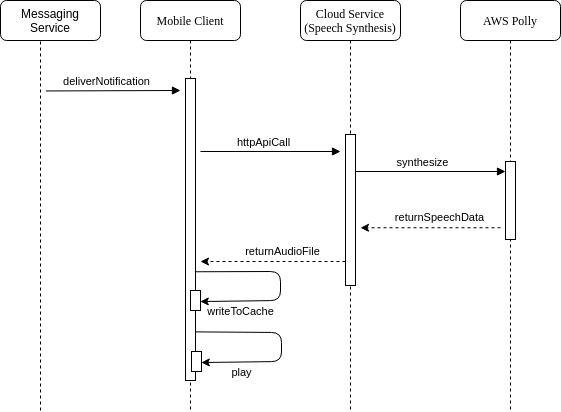
\includegraphics[width=\textwidth]{graphics/diagramms/Sequence_Speech_Synth_System}
        \caption{Sequenzdiagramm - Sprachsynthese auf Systemebene}
    \end{minipage}
\end{figure}


Nachdem eine empfangene Benachrichtigung der Inbox hinzugefügt wurde, wird geprüft ob Sprachsynthese in den lokalen Einstellungen aktiviert ist.
Ist diese deaktiviert, endet die Verarbeitung.
Andernfalls wird geprüft, ob das ''isTextToSpeech'' Flag auf der Benachrichtigung aktiviert ist.
Nur wenn das Flag aktiviert ist, wird die Benachrichtigung an den SpeechSynthesisService übergeben.
Der SpeechSynthesisService prüft als erstes, ob die Sprachdaten für die empfangene Benachrichtigung bereits lokal zur Verfügung stehen.
Dies wird gemacht in dem er überprüft, ob im Applikationsverzeichnis bereits eine Datei für Id, Version und Sender der Benachrichtigung vorhanden ist.
Ist dies der Fall, werden die Inhalte dieser Datei abgespielt und es wird keine Anfrage an den Cloudservice versendet.
Wenn die Daten gar nicht oder nur in einer anderen Version lokal gefunden werden, wird eine Anfrage an den CloudService gesendet.

Sobald Sprachdaten über die Cloudservice API angefragt werden, lädt dieser den Namen des Senders und die Inhalte der Benachrichtigung aus der Konfiguration.
Anschliessend sendet der Cloudservice eine Anfrage an Amazon Polly, um Titel und Sender der Benachrichtigung als Sprachdaten zu synthetisieren.
Die Resultate von Amazon Polly werden als Resultat der Anfrage des Mobile Clients zurückgegeben.
Der Client speichert die empfangenen Daten lokal im Applikationsverzeichnis.
Nachdem die Daten gespeichert wurden, wird deren Inhalt abgespielt.

\clearpage

\subsection{Gegensprechanlage}

Mit der Integration von synchroner Sprachübertragung wird das Praxisrufsystem um die Funktion Gegensprechanlage erweitert.
Die gewählte Technologie WebRTC erlaubt es, Sprachverbindungen zwischen Clients aufzubauen.
Dieses Kapitel beschreibt wie das Praxisrufsystem erweitert wird, um eine konfigurierbare Gegensprechanlage mit WebRTC zu implementieren.

\subsubsection{Konfiguration}

Die Gegensprechanlage wird in den nativen Mobile Client integriert.
Praxismitarbeitende können über Buttons Sprachverbindungen zu anderen Clients aufbauen.
Welche Buttons und damit welche Sprachverbindungen zur Verfügung stehen, wird durch Praxisadministrierende über das Admin UI konfiguriert.
Damit dies möglich ist, sind Änderungen an de Configuration-Modul des Cloudservice sowie am Admin UI notwendig.

Die Konfiguration von Mobile Clients wird in der Domäne Configuration abgebildet.
Zentral sind dabei die beiden Entities Client und ClientConfiguration.
Ein Client repräsentiert ein physisches Endgerät.
Eine ClientConfiguration definiert die Konfiguration eines Gerätes.

Praxisruf bietet bereits heute die Möglichkeit Buttons zu konfigurieren, über welche Benachrichtigungen versendet werden können.
Diese Buttons werden mit der Entität NotificationType konfiguriert, welche wiederum einer ClientConfiguration zugeordnet werden können.
Diese ClientConfiguration wird bei der Anmeldung auf dem Mobile Client geladen und verwendet, um die nötigen Buttons darzustellen.
Für die Konfiguration von Sprachverbindungen wird die Entität CallType erstellt.
Ein CallType beinhaltet den Text, welcher auf dem zugehörigen Button auf Clientseite angezeigt wird und eine Liste von Clients, welche als Ziel der Sprachverbindung verwendet werden.
Abbildung 7.14 zeigt einen Ausschnitt aus dem Entity Relationship Diagramm der Configuration Domäne.
Dabei sind die Teile, die für die Konfiguration von Sprachverbindungen ergänzt werden, grün markiert.

\begin{figure}[h]
    \centering
    \begin{minipage}[b]{0.7\textwidth}
        \fbox{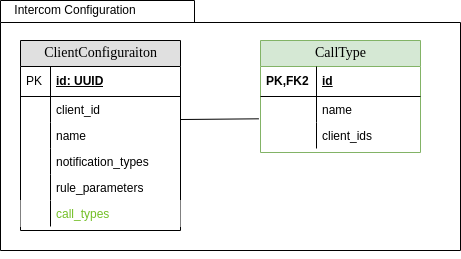
\includegraphics[width=\textwidth]{/home/joshua/FHNW/dev/IP6/IP6_Bachelorarbeit_Bericht_Cloudbasiertes_Praxisrufsystem/src/graphics/diagramms/erd_intercom_v02.drawio}}
        \caption{ERD Ausschnitt - Konfiguration Gegensprechanlage}
    \end{minipage}
\end{figure}

Das Admin UI wird mit Ansichten erweitert, über welche CallTypes erstellt, angezeigt, bearbeitet und gelöscht werden können.
Gleichzeitig wird der Cloudservice um Rest Endpunkte für das Lesen, Erstellen, Aktualisieren und Löschen von CallTypes erweitert.
Die Ansichten für ClientConfigurations im Admin UI werden so erweitert, dass CallTypes darauf angezeigt, hinzugefügt und entfernt werden können.
Die API des Cloudservice wird erweitert, um die erweiterte Konfiguration verwalten zu können.

\clearpage

\subsubsection{Signaling Instanz}

Mit WebRTC werden Peer-To-Peer Verbindungen aufgebaut~\cite{webrtc}.
Damit diese Verbindungen aufgebaut werden können, müssen die beteiligten Geräte Signalmeldungen austauschen können.
Dazu ist eine Instanz notwendig, welche Signale zwischen den Endgeräten vermitteln kann.
Diese Signaling Instanz wird als Teil des Cloudservice implementiert.

Der Cloudservice wird um ein neues Modul ''Signaling'' erweitert.
Dieses soll den Austausch von Signalen zwischen Clients ermöglichen.
Gleich wie das Modul für Sprachsynthese wird es unabhängig von den anderen Domänenmodulen im Cloudservice implementiert.
Das Modul Signaling muss dabei zwei Aufgaben übernehmen.
Erstens muss es Mobile Clients die Möglichkeit bieten, sich für Sprachverbindungen zu registrieren.
Zu diesem Zweck müssen Mobile Clients eine Verbindung mit der Signaling Instanz herstellen und trennen können.
Zweitens muss es Signalmeldungen empfangen und an die relevanten Empfänger zustellen können.
Kann eine Signalmeldung nicht zugestellt werden, muss es den betroffenen Empfänger über das verpasste Signal informieren.

Für diese Funktionen wird das Interface ClientConnector definiert.
Dieses definiert die Methoden afterConnectionEstablished und afterConnectionClosed.
Die beiden Methoden werden aufgerufen, wenn eine Verbindung geöffnet bzw.\ geschlossen wurde.
Die Implementierung dieses Interfaces ist dafür verantwortlich verfügbare Verbindungen zu verwalten.
Weiter definiert das Interface die Methode handleSignal.
Diese muss verwendet werden, um ein Signal entgegenzunehmen und an relevante Empfänger weiterzuleiten.

\begin{figure}[h]
    \centering
    \begin{minipage}[b]{1\textwidth}
        \fbox{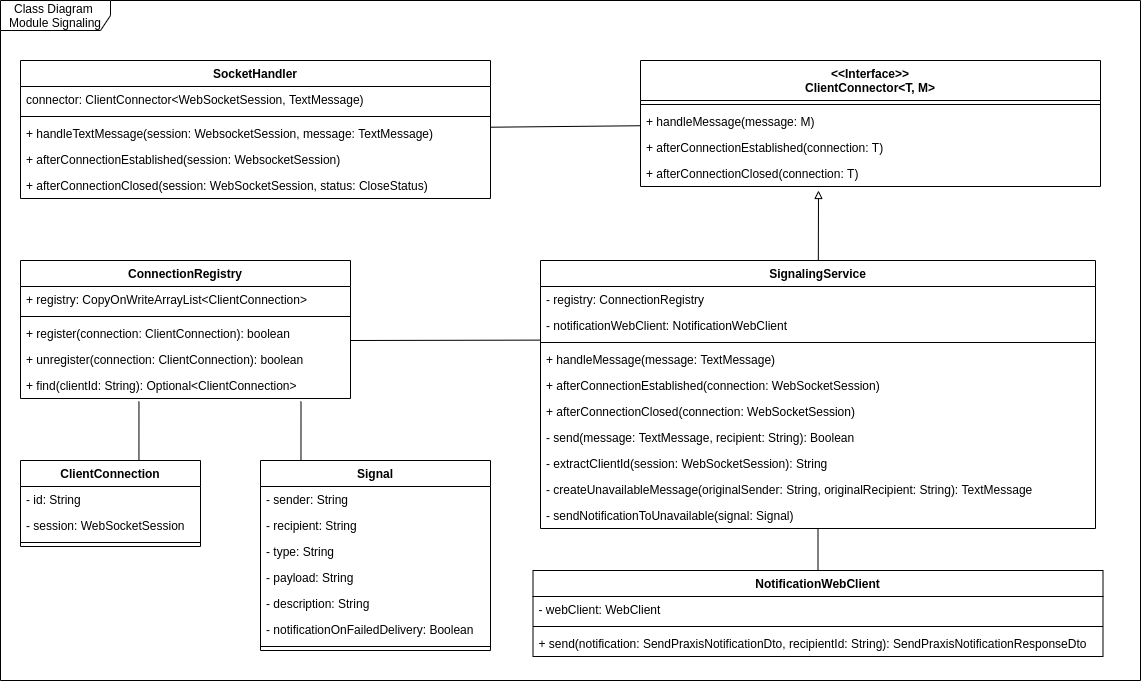
\includegraphics[width=\textwidth]{/home/joshua/FHNW/dev/IP6/IP6_Bachelorarbeit_Bericht_Cloudbasiertes_Praxisrufsystem/src/graphics/diagramms/Class_Intercom_Full_V01}}
        \caption{Klassendiagramm - Modul Signaling}
    \end{minipage}
\end{figure}

Für die Verwaltung von Verbindungen wird die Komponente ConnectionRegistry implementiert.
Diese führt eine Liste bekannter Verbindungen und bietet Methoden um Verbindungen zu registrieren und wieder entfernen.
Sie bietet weiter eine Methode, um zu überprüfen, ob eine bestimmte Verbindung bekannt ist.
Bekannte Verbindungen werden mit der Klasse ClientConnection abgebildet.
Ein ClientConnection beinhaltet immer einen Identifikator und das technische Verbindungsobjekt.
So können Verbindungen in der ClientConnection immer über einen eindeutigen Identifikator registriert und gefunden werden.

Die Klasse SignalingService implementiert das ClientConnector Interface.
Sie verwendet die Klasse ConnectionRegistry, um eine Liste von verfügbaren Verbindungen zu führen.
Über die Methoden onConnectionEstablished werden neue Verbindungen in der ConnectionRegistry registriert.
Mit der Methode onConnectionClosed werden geschlossene Verbindungen wieder entfernt.

Für das Zustellen von Signalen über bekannte Verbindungen wird die Methode handleSignal implementiert.
Jedes Signal beinhaltet die Identifikation seines Empfängers.
Beim Empfang eines Signals wird kontrolliert, ob die ConnectionRegistry eine Verbindung für die Identifikation des Empfängers enthält.
Ist dies der Fall, wird das Signal über diese Verbindung an den Empfänger übermittelt.
Wenn dies nicht der Fall ist oder wenn das Senden des Signals fehlschlägt, ist der Empfänger nicht erreichbar.
Nicht erreichbare Empfänger werden mit Benachrichtigungen über verpasste Signale informiert.
Dazu wird eine Benachrichtigung über die API des Moduls Notification versendet.

Die Schnittstelle der Signaling Instanz im Cloudservice wird mit Websockets umgesetzt.
Dazu wird die Bibliothek Spring-Boot-Starter-Websocket verwendet.
Es wird ein WebsocketHandler implementiert, welcher unter dem Pfad ''$<$serverUrl$>$/signaling'' erreichbar ist.
Etablierte Verbindungen müssen eindeutig einem Client zugeordnet werden können.
Diese Identifikation wird als Query Parameter bei Verbindungsaufbau mitgegeben.
Der WebsocketHandler definiert Methoden die beim Öffnen und Schliessen von Verbindungen sowie beim Empfang von Signalen aufgerufen werden.
Die Verarbeitung dieser Signale und Verbindungen wird an den SignalingService delegiert.

\subsubsection{Sicherheit für Signaling}

Der Zugriff auf die Signaling Instanz und die darüber ausgetauschten Signale darf nur für Berechtigte möglich sein.
Um dies sicherzustellen, wird der Verbindungsaufbau nur erlaubt, wenn die Anfrage dazu authentisiert ist.
Für die Authentisierung wird derselbe Mechanismus wie für Http-Anfragen der Cloudservice-API verwendet.
Durch die Konfiguration des Cloudservices wird die Authentifizierung aller Http Requests überprüft.
Mit dieser Prüfung wird sichergestellt, dass gültige Authentifizierungsdaten im Header der Anfrage vorhanden sind.
Ist dies nicht der Fall, wird eine entsprechende Fehlermeldung zurückgegeben.
Bei der Prüfung von Http-Anfragen durch den Cloudservice werden weiter die Rollen, welche dem Aufrufer zugeteilt sind ausgelesen.

Diese Prüfung der Authentifizierung wird auch für die Http-Anfragen, welche zum Aufbau einer Websocketverbindung nötig sind ausgeführt.
Beinhaltet eine Anfrage zum Aufbau einer Websocketverbindung keine gültige Authentifizierung, wird eine Fehlermeldung zurückgegeben.
Der Aufbau der Websocketverbindung wird abgebrochen.

Die Prüfung der ausgelesenen Rollen wird mit der Klasse HttpSessionHandshakeInterceptor implementiert.
Diese wird, nachdem eine Anfrage zum Aufbau einer Websocketverbindung eingegangen ist, aufgerufen.
Der HttpSessionHandshakeInterceptor erlaubt es die Anfrage zum Verbindungsaufbau auszulesen.
Dies erlaubt es hier zu verifizieren, dass der Request authentifiziert wurde und nur die zugeteilten Rollen zu überprüfen.
Praxisruf kennt die zwei Rollen ''ADMIN'' und ''USER''.
Beide Rollen sind berechtigt, dass Rufsystem über den Mobile Client zu verwenden und dürfen damit Signalmeldungen austauschen.
Hat der Aufrufer keine dieser Rollen, wird der Verbindungsaufbau abgebrochen.

Für Websocketverbindungen wird ausschliesslich das Protokoll Secure WebSockets (WSS) verwendet.
Die Http-Anfragen für den Verbindungsaufbau werden ausschliesslich über Https versendet.
Der Verbindungsaufbau und Austausch von Signalmeldungen über das Signaling Modul sind damit verschlüsselt.

\clearpage

\subsubsection{Anmeldung und Registrierung}

Dieses Kapitel beschreibt, welche Anmelde- und Registrierungsprozesse im Mobile Client benötigt werden.

Anmeldung und Registrierung für Benachrichtigungen funktionieren mit dem neuen Mobile Client nach demselben Ablauf wie im Vorgängerprojekt.
Die Registrierung für Sprachverbindungen beim Signaling Modul des Cloudservice wird mit diesem Projekt hinzugefügt.
Der gesamte Ablauf von Anmeldung und Registrierung wird in Abbildung 7.16 dargestellt.
Praxismitarbeitende öffnen die Applikation und geben ihr Benutzername und Passwort ein.
Der Mobile Client verwendet diese, um sich über Basic Authentication beim Cloudservice anzumelden.
Als Antwort auf die Anmeldung gibt der Cloudservice ein Json Web Token (JWT) zurück.
Dieses wird lokal auf dem Gerät gespeichert und für alle weiteren Anfragen an den Cloudservice verwendet.
Nachdem die Anmeldung erfolgt ist, wird eine Liste der verfügbaren Konfigurationen geladen.
Der Benutzer wählt die gewünschte Konfiguration aus und bestätigt.

\begin{figure}[h]
    \centering
    \begin{minipage}[b]{0.9\textwidth}
        \fbox{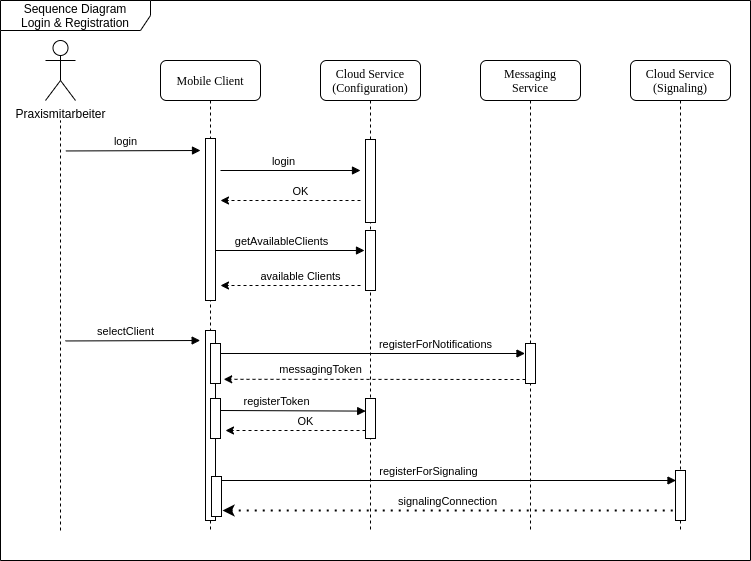
\includegraphics[width=\textwidth]{/home/joshua/FHNW/dev/IP6/IP6_Bachelorarbeit_Bericht_Cloudbasiertes_Praxisrufsystem/src/graphics/diagramms/Sequence_Registration}}
        \caption{Sequenzdiagramm - Anmeldung und Registrierung im Mobile Client}
    \end{minipage}
\end{figure}

Danach wird diese Konfiguration geladen und die Hauptansicht angezeigt.
Die geladene Konfiguration beinhaltet alle Informationen die nötig sind um Buttons für Benachrichtigungen und Sprachverbindungen anzuzeigen.
Im Hintergrund muss sich der Mobile Client nun für Benachrichtigungen und Sprachverbindungen registrieren.
Für Benachrichtigungen registriert er sich zuerst bei Firebase Cloud Messaging.
Er erhält ein Token, welches den Client beim Messaging Service identifiziert.
Dieses Token sendet der Mobile Client zusammen mit der gewählten Konfiguration an den Cloudservice.
Dieser persistiert die Registrierung und kann sie verwenden, um Benachrichtigungen an diesen Client zuzustellen.
Für Sprachverbindungen muss zudem eine Verbindung zum Signaling Modul des Cloudservices aufgebaut werden.
Dazu wird wie in Kapitel 7.4.6 beschrieben eine Websocketverbindung geöffnet.

\clearpage

\subsubsection{Signalmeldungen}

Dieses Kapitel beschreibt die Signalmeldungen, welche in Praxisruf verwendet werden.
Dabei wird beschrieben wie diese aufgebaut sind und welchen Rolle sie im System erfüllen.
Abbildung 7.17 zeigt, wie Signalmeldungen im Mobile Client modelliert werden.

\begin{figure}[h]
    \centering
    \begin{minipage}[b]{0.5\textwidth}
        \fbox{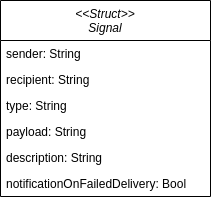
\includegraphics[width=\textwidth]{graphics/diagramms/Class_Signal}}
        \caption{Klassendiagramm - Signal}
    \end{minipage}
\end{figure}

Alle Signalmeldungen beinhalten Identifikation von Sender und Empfänger.
Diese werden von der Signaling Instanz verwendet, um die Signale korrekt weiterzuleiten.
Die Werte Type, Payload und Description werden im Mobile Client verwendet, um das Signal korrekt zu verarbeiten und Verbindungen aufzubauen.
Das Flag notificationOnFailedDelivery wird im Cloudservice ausgewertet.
Wenn ein Signal nicht zugestellt werden kann und dieses Flag aktiviert ist, wird der Empfänger mit einer Benachrichtigung darüber informiert.
Dazu wird die API des Notification Moduls des Cloudservices verwendet.

Praxisruf verwendet sechs Typen von Signalmeldungen.
Folgende Übersicht beschreibt pro Typ welche Daten ein Signal beinhaltet und welche Rolle es erfüllt.
\\
\begin{tabbing}
    Left \= Middle \= Right \= Right \kill
    Offer
    \> \> \> Wird vom Initiator der Sprachverbindung an die Empfänger gesendet. Ein Offer
    \\\> \> \> beinhaltet die SDP Informationen des Initiators und initiiert eine Verbindung. \\ \\

    Answer
    \> \> \> Wird vom Empfänger eines Offers an den Initiator der Sprachverbindung gesendet.
    \\\> \> \> Es beinhaltet SDP Informationen des Empfängers und bestätigt eine Verbindung. \\ \\

    Ice Candidate
    \> \> \> Beinhaltet Informationen eines ICE Candidates, die für den Verbindungsaufbau ver-
    \\ \> \> \> wendet werden. Nach Verarbeitung von Offer und Answer tauschen Initiator und
    \\ \> \> \> Empfänger solange Ice Candidate Signale aus, bis sie sich auf einen Kandidaten
    \\ \> \> \> geeinigt haben. Dieser wird verwendet, um die Verbindung aufzubauen.
    \\ \> \> \> \\

    End
    \> \> \> Wird versendet, nachdem die Verbindung durch tippen des Auflegen-Button in der
    \\ \> \> \> Applikation beendet wurde. Empfang dieses Signal führt dazu, dass offene Sprach-
    \\ \> \> \> verbindungen zum Sender dieses Signals beim Empfänger beendet werden.\\ \\

    Unavailable
    \> \> \> Wenn der Signalingserver ein Signal nicht zustellen kann, wird ein Unavailable-
    \\ \> \> \> Signal zurück an den Sender gesendet. Der Sender ist so informiert, dass die Ver-
    \\ \> \> \> bindung zum Gesprächspartner nicht aufgebaut wurde. \\ \\

    Decline
    \> \> \> Wird ein Offer empfangen während die Gegensprechanlage in den lokalen Einstel-
    \\ \> \> \> lungen deaktiviert ist oder bereits in Anruf aktiv ist, sendet der Mobile Client ein
    \\ \> \> \> Decline Signal zurück. Der Sender ist so informiert, dass die Verbindung zum Ge-
    \\ \> \> \> sprächspartner abgelehnt wurde.
\end{tabbing}

\clearpage

\subsubsection{Verbindungsaufbau}

Praxismitarbeitende können Sprachverbindungen zu anderen Clients aufbauen indem sie auf den entsprechenden Button in der Praxisruf App tippen.
Zum Zeitpunkt an dem der Button getippt wird, weiss der Mobile Client noch nicht, zu welchen Clients diese Verbindung aufgebaut werden soll.
Als Erstes muss deshalb beim Cloudservice angefragt werden, zu welchen Clients eine Sprachverbindung aufgebaut werden soll.
Der Cloudservice bietet dazu einen Endpoint an, über den der vollständige CallType des verwendeten Buttons geladen werden kann.
Nachdem diese Informationen geladen sind, können Sprachverbindungen zu allen Empfängern aufgebaut werden.
Dazu müssen Offer, Answer und Ice Candidate Signale ausgetauscht werden.
Der auslösende Client initialisiert die Peer-to-Peer Verbindung auf seiner Seite und sendet für jeden Gesprächspartner ein Offer.
Der Cloudservice findet die Verbindung der jeweiligen Empfänger und leitet die Signale über deren Verbindung weiter.

Nach Eingang des Offer-Signals wird die Verbindung auf Empfängerseite initialisiert und eine Answer zurück an den Initiator gesendet.
Diese wird gleich wie das Offer-Signal über die Signaling Instanz zugestellt.
Der Initiator empfängt die Antwort Signale und ergänzt die notwendigen Verbindungsinformationen.
Abbildung 7.18 visualisiert diesen Ablauf.

\begin{figure}[h]
    \centering
    \begin{minipage}[b]{0.9\textwidth}
        \fbox{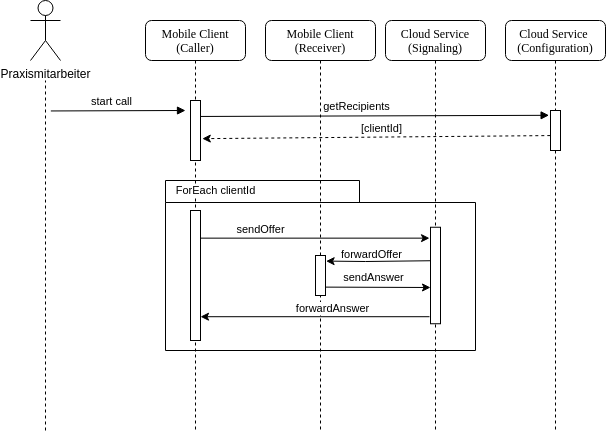
\includegraphics[width=\textwidth]{graphics/diagramms/Sequence_Intercom_Broking_V02}}
        \caption{Sequenzdiagramm - Verbindungsaufbau mit Offer und Answer Signalen}
    \end{minipage}
\end{figure}

Nachdem die Offer und Answer Meldungen ausgetauscht sind, müssen Ice Candidate Meldungen ausgetauscht werden.
Der Austausch von Ice Candidate Meldungen wird so lange wiederholt, bis sich beide Seiten einer Verbindung auf Verbindungsdetails geinigt haben.
Sobald dieser Austausch beendet ist, besteht die Verbindung und es können Sprachdaten ausgetauscht werden.

\clearpage

\subsubsection{Anbindung Mobile Client an Singaling Instanz}

Dieses Kapitel beschreibt, wie Websockeverbindungen zum Austausch von Signalmeldungen in den nativen Mobile Client integriert werden.

In Kapitel 7.2 wird die Klasse PraxisrufApi beschrieben.
Diese implementiert die Anbindung and die Http-API des Cloudservice.
Um Signalmeldungen über die Signaling Instanz des Cloudservice auszutauschen, müssen Websockets verwendet werden.
Damit die Anbindung an alle Schnittstellen des Cloudservice einheitlich bleibt, wird PraxisrufApi erweitert, um auch Websocketverbindungen zu unterstützen.
Dies beinhaltet den Auf- und Abbau von Verbindungen, sowie das Senden und Empfangen von Meldungen über diese Verbindung.
Weiter müssen Verhalten beim Empfang von Fehlermeldungen und dem unerwarteten Schliessen der Verbindung definiert werden.

Der Austausch von Signalmeldungen ist der einzige Anwendungsfall für Websockets in Praxisruf.
Deshalb wird auf eine generische Integration von Websockets verzichtet.
Zur Erweiterung von PraxisrufApi werden die Extension PraxisrufApi+Signaling und das Protokoll PraxisrufApiSignalingDelegate definiert.
Diese setzen die Anbindung von Websockets für den Austausch von Signalmeldungen um.

\begin{figure}[h]
    \centering
    \begin{minipage}[b]{0.6\textwidth}
        \fbox{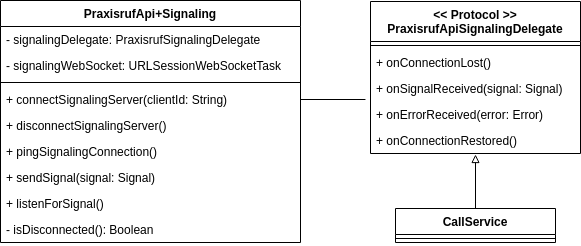
\includegraphics[width=\textwidth]{graphics/diagramms/Class_Mobile_Client_Signaling_Connection}}
        \caption{Klassendiagramm - Signaling Schnittstelle in Mobile Client}
    \end{minipage}
\end{figure}

Die Extension PraxisrufApi+Signaling ist für die Verbindung zu der Signaling Instanz verantwortlich.
Für die Integration dieser Extension in den Rest der Applikation wird das Protokoll PraxisrufApiSignalingDelegate definiert.
Zum Aufbau der Verbindung zu der Signaling Instanz wird die Methode connectSignalingServer definiert.
Die Identifikation des Clients wird bei dieser Abfrage als Parameter mitgegeben.
So kann die Verbindung von der Signaling Instanz eindeutig einem Client zugeordnet werden.
Nachdem die Verbindung geöffnet ist, können Signale empfangen und verarbeitet werden.
Dies wird durch die Methode listenForSignal initialisiert.
Darin wird der Websocketverbindung signalisiert, dass der Client bereit ist die nächste Meldung zu empfangen.
Sobald eine Meldung empfangen wird, wird diese über den PraxisrufApiSignalingDelegate verarbeitet.
Wurde eine gültige Signalmeldung empfangen, wird diese über die Methode onSignalReceived verarbeitet.
Wurde hingegen eine ungültige Signalmeldung oder eine Fehlermeldung empfangen wird die Methode onErrorReceived aufgerufen.
Im Fehlerfall wird zudem überprüft, ob die Verbindung noch offen verwendbar ist.
Sollte die Verbindung nicht mehr verwendbar sein, wird die Methode onConnectionLost des Delegates aufgerufen.
Dadurch wird versucht, die Verbindung erneut aufzubauen.
Ist dies nicht möglich, wird eine Fehlermeldung angezeigt. 

PraxisrufApi+Signaling definiert weiter Methoden um Signal- und Pingmeldungen zu versenden.
Pingmeldungen werden in Regelmässigen Abständen gesendet um sicherzustellen, dass die Verbindung zu der Signaling Instanz geöffnet bleibt.
Vor dem Senden jeder Meldung wird geprüft, ob die Verbindung zur Signaling Instanz verwendbar ist.
Ist dies nicht der Fall, wird die Methode onConnectionLost des Delegates aufgerufen und anschliessend versucht die Meldung zu versenden.
Schlägt das Senden fehl, wird die Methode onErrorReceived auf dem Delegate aufgerufen.

Die Methoden des Protokolls CallClientDelegate werden durch die Klasse CallService implementiert.
Der CallService vermittelt Anfragen zwischen Signaling Instanz, Benutzeroberfläche und Peer-To-Peer Verbindungen im Mobile Client.
Er ist dafür verantwortlich Signale an die Peer-To-Peer Verbindung weiterzuleiten, geschlossene Verbindungen wieder zu öffnen und Fehlermeldungen anzuzeigen.
Empfangene Signalmeldungen werden über die Methode onSignalReceived an die Komponente CallClient übergeben (Siehe Kapitel 7.4.9).
Die Methoden onConnectionLost und onErrorReceived werden verwendet, um Fehlermeldungen anzuzeigen und geschlossene Verbindungen erneut zu öffnen.
Nachdem die Verbindung zur Signaling Instanz verloren gegangen ist, wird bis zu zehnmal versucht, die Verbindung erneut zu öffnen.
Wenn die Verbindung dadurch nicht repariert werden kann, wird sie geschlossen und dem Benutzer eine Fehlermeldung angezeigt.

\subsubsection{Verbindungsverwaltung}

Dieses Kapitel beschreibt, wie im Mobile Client sichergestellt wird, dass die Verbindung zu der Signaling Instanz langfristig zur Verfügung steht.
Abbildung 7.20 gibt einen Überblick, über die Abläufe dazu umgesetzt werden.
Dieser Ablauf ist mit den Komponenten CallService und PraxisrufApi+Signaling die, in Kapitel 7.4.7 beschrieben sind, implementiert.

\begin{figure}[h]
    \centering
    \begin{minipage}[b]{1\textwidth}
        \fbox{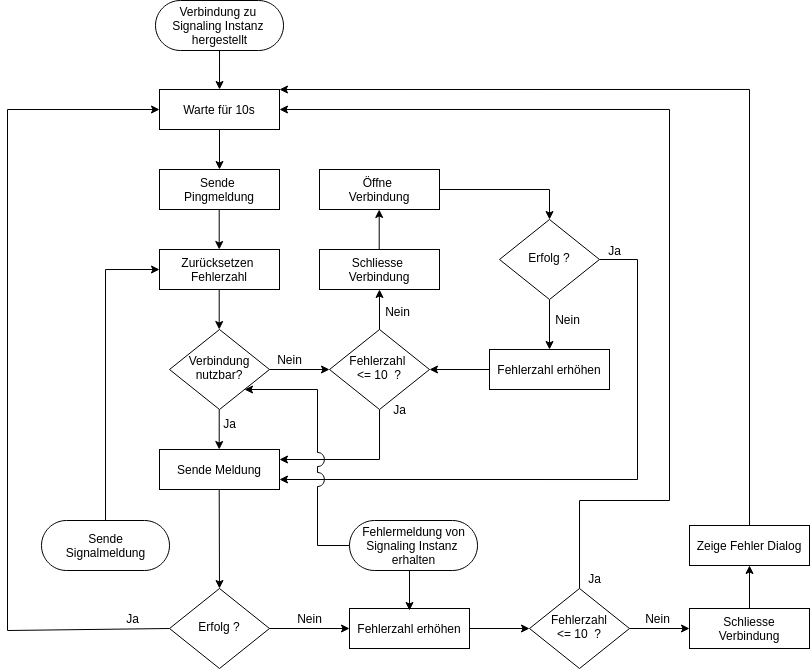
\includegraphics[width=\textwidth]{graphics/diagramms/flow_connection}}
        \caption{Flowchart - Verbindungsverwaltung}
    \end{minipage}
\end{figure}

Um festzustellen, ob die eine getrennte Verbindung repariert werden kann, wird im CallService ein Fehlerzähler geführt.
Dieser wird beim Start der Applikation mit null initialisiert und bei jedem Verbindungsfehler um eins inkrementiert.
Ein Verbindungsfehler tritt auf, wenn eine Fehlermeldung über die Signaling Verbindung empfangen wird und wenn das Senden einer Meldung oder das Wiederherstellen der Verbindung fehlschlägt.

Die Verbindung zur Signaling Instanz wird hergestellt, sobald die Applikation gestartet wird.
Nachdem die Verbindung hergestellt wurde, werden im Abstand von zehn Sekunden Pingmeldungen über die Verbindung gesendet.
Dadurch wird sichergestellt, dass die Verbindung geöffnet bleibt.
Vor dem Versenden jeder Meldung wird der Fehlerzähler zurückgesetzt und es wird überprüft, ob die Verbindung verwendet werden kann.
Ist die Verbindung fehlerhaft, werden bis zu zehn Versuche unternommen, sie wiederherzustellen.
Anschliessend wird versucht, die Meldung zu versenden.
Wenn die Meldung erfolgreich versendet wurde, wird der Fehlerzähler zurückgesetzt und zehn Sekunden gewartet, bis die nächste Pingmeldung versendet wird.
Andernfalls wird die Fehlerzahl um eins erhöht.
Ist die Fehlerzahl danach grösser als zehn, wird die Verbindung getrennt.
In der Benutzeroberfläche wird ein Fehlerdialog angezeigt.
Die Verbindung bleibt geschlossen bis die nächste Meldung versendet wird.
Dies der Fall, wenn das Interval für die nächste Pingmeldung abgelaufen ist oder wenn ein Anruf über die Benutzeroberfläche gestartet wird.

Bei Start eines Anrufes aus der Benutzeroberfläche werden dieselben Prüfungen, wie vor dem Versenden von Pingmeldungen ausgeführt.
So werden geschlossene Verbindungen zur Signaling Instanz frühzeitig repariert.
Weiter wird nach Empfang jedes Fehlers über die Signaling Verbindung geprüft, ob diese noch offen ist.
Ist dies nicht der Fall, werden auch hier bis zu zehn Versuche unternommen, die Verbindung wiederherzustellen.

Dieser Ablauf stellt sicher, dass die Verbindung zu der Signaling Instanz geöffnet bleibt und wenn nötig repariert wird.
Wenn möglich, geschieht dies direkt nach Verbindungsverlust.
Andernfalls werden Praxismitarbeitende informiert, dass die Verbindung nicht hergestellt werden konnte.
Im Hintergrund wird in dieser Situation regelmässig versucht, die Verbindung zu reparieren.
Die Bedienelemente für die Gegensprechanlage bleiben während dieser Zeit aktiviert und können weiter verwendet werden.
Wenn Praxismitarbeitende einen Anruf starten und die Verbindung immer noch getrennt ist, wird die sie frühzeitig wiederhergestellt.
Ist dies erfolgreich, wird der Anruf gestartet.
Andernfalls wird erneut ein Fehlerdialog angezeigt.

\clearpage

\subsubsection{Sprachverbindungen im Mobile Client}

Dieses Kapitel beschreibt wie WebRTC-Komponenten in den Mobile Client integriert werden, um Sprachverbindungen zu ermöglichen.

Für die Integration der WebRTC-Komponenten wird eine Klasse CallClient und ein Protokoll CallClientDelegate erstellt.
Der CallClient verwaltet Sprachverbindungen, während der Delegate zur Integration mit der restlichen Applikation dient.
Abbildung 7.21 zeigt das Klassendiagramm beider Komponenten.
Die Methoden des CallClientDelegate-Protokolls werden von der Klasse CallService implementiert.
Da diese Klasse auch das Protokoll SignalingDelegate implementiert, kann sie verwendet werden um Signalmeldungen zwischen CallClient und PraxusrufApi+Signaling zu vermitteln.

\begin{figure}[h]
    \centering
    \begin{minipage}[b]{0.6\textwidth}
        \fbox{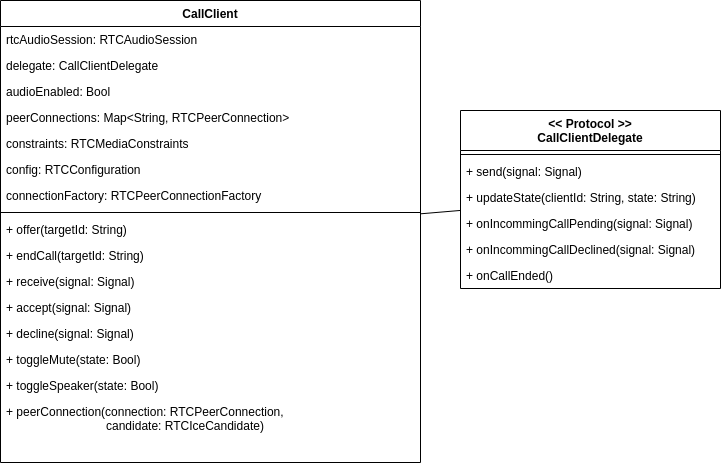
\includegraphics[width=\textwidth]{graphics/diagramms/Class_Mobile_Client_Signal_Processing}}
        \caption{Klassendiagramm - CallClient und CallClientDelegate}
    \end{minipage}
\end{figure}

Für den Aufbau von ausgehenden Verbindungen wird eine RTCPeerConnection im CallClient des Senders initialisiert.
Es werden die SDP Informationen für Beschreibung der Verbindung erstellt und mit einem Offer-Signal an den Empfänger gesendet.
Dieses Offer-Signal wird über den CallClientDelegate versendet, welcher das Signal an die Signaling Instanz zustellt.

Für den Aufbau von eingehenden Verbindungen wird das Offer-Signal über die Methode receive empfangen.
Dabei wird die Verbindung nicht direkt initialisiert.
Stattdessen wird das Signal zwischengespeichert und die Methode onIncommingCallPending des Delegates aufgerufen.
Die Implementation des CallClientDelegate navigiert darauf zu der Ansicht für aktive Anrufe und meldet dem CallClient über die Methode acceptPending, dass die Verbindung initialisiert werden soll.
Der CallClient initialisiert darauf eine RTCPeerConnection und sender ein Answer Signal über die send Methode.

Answer-Signale werden ebenfalls über die receive Methode im CallClient empfangen.
Beim Empfang einer Answer werden die SDP Informationen auf der lokalen RTCPeerConnection ergänzt.

Neben dem Austausch von Offer- und Answer-Signalen müssen Ice Candidate Signale ausgetauscht werden können.
Sobald ein Ice Candidate zur Verfügung steht, erstellt der CallClient ein entsprechendes Signal und sendet es an den Empfänger.
Damit dies möglich ist, muss der CallClient über verfügbare Ice Candidates informiert werden.
Die WebRTC Bibliothek bietet dazu das Protokoll RTCPeerConnectionDelegate.
Dieses kann auf der RTCPeerConnection registriert werden und wird aufgerufen, sobald ein neuer Ice Candidate verfügbar ist.
Der CallClient implementiert dieses Protokoll und registriert sich auf allen RTCPeerConnections als Delegate.

Sprachverbindungen müssen über die Benutzeroberfläche verwaltet werden können.
Der CallClient bietet deshalb Methoden an, um eine Verbindung zu starten und beenden.
Weiter bietet er die Möglichkeit Mikrofon und Lautsprecher für geöffnete Verbindungen stummzuschalten.
Bei eingehenden Verbindungen, dem Beenden von Anrufen und Veränderungen am Status einer Verbindung, muss die Benutzeroberfläche informiert werden.
Der CallClientDelegate definiert dazu Methoden über welche der CallClient diese Informationen weitergeben kann.

\subsubsection{Signalverarbeitung im Mobile Client}

Peer-To-Peer Sprachverbindungen werden über die Komponenten CalService, CallClient und PraxisrufApi+Signaling in den Mobile Client integriert.
Dieses Kapitel beschreibt den Kommunikationsablauf zwischen diesen Komponenten anhand des Austauschs von Offer- und Answer-Signalen.

\begin{figure}[h]
    \centering
    \begin{minipage}[b]{0.85\textwidth}
        \fbox{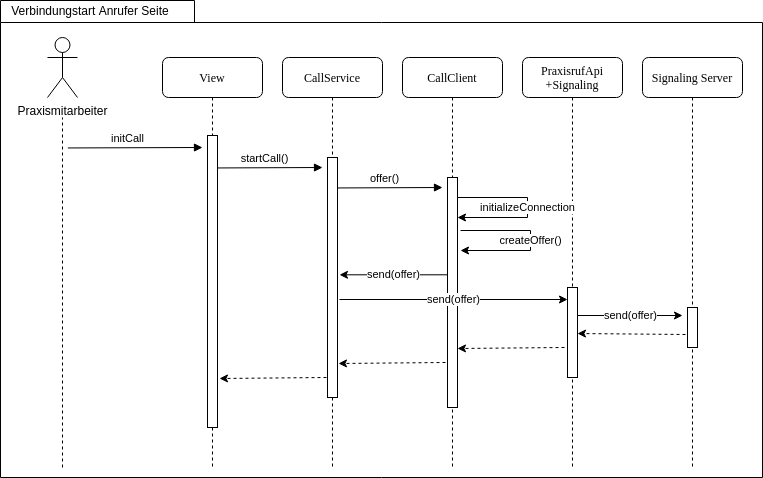
\includegraphics[width=\textwidth]{/home/joshua/FHNW/dev/IP6/IP6_Bachelorarbeit_Bericht_Cloudbasiertes_Praxisrufsystem/src/graphics/diagramms/Sequence_MobileClient_Caller_Signaling.drawio}}
        \caption{Sequenzdiagramm - Initialisierung Sprachverbindung auf Senderseite }
    \end{minipage}
\end{figure}


Die Klassen CallClient und PraxisrufApi+Signaling definieren je ein Delegate-Protokoll.
Diese Protokolle definieren die Funktionen, über welche die Komponenten Informationen weitergeben können.
Die Klasse CallService implementiert beide Delegate-Protokolle.
Er erstellt Instanzen von CallClient und PraxisrufApi+Signaling und registriert sich anschliessend bei beiden als Delegate.
Der CallService selbst wird in den View Komponenten der Applikation verwendet.
Er nimmt Benutzereingaben entgegen und delegiert die entsprechende Funktionalität an den CallClient und PraxisrufApi+Signaling.
Er nimmt ausserdem Informationen von CallClient und PraxisrufApi+Signaling entgegen und stellt Anzeigeinformationen für die Benutzeroberfläche zur Verfügung.

Abbildung 7.22 zeigt die Kommunikation zwischen den beteiligten Komponenten bei der Initialisierung einer Sprachverbindung auf Empfängerseite.
Dabei wird der Ablauf von Benutzerinteraktion des Senders bis zum Senden des Offer-Signals dargestellt.
Sobald Praxismitarbeitende einen Anruf startet, wird die View für aktive Anrufe geladen.
Diese initialisiert den Anruf über den CallService.
Der CallService ruft dazu als Erstes den CallClient auf.
Der CallClient initialisiert die lokalen Verbindungsinformationen und erstellt ein Signal, um den Empfänger zu informieren.
Dieses Signal gibt er an den CallService weiter.
Der CallService leitet das Signal an den PraxisrufApi+Signaling weiter, welcher das Versenden an den Cloudservice übernimmt.

\begin{figure}[h]
    \centering
    \begin{minipage}[b]{0.85\textwidth}
        \fbox{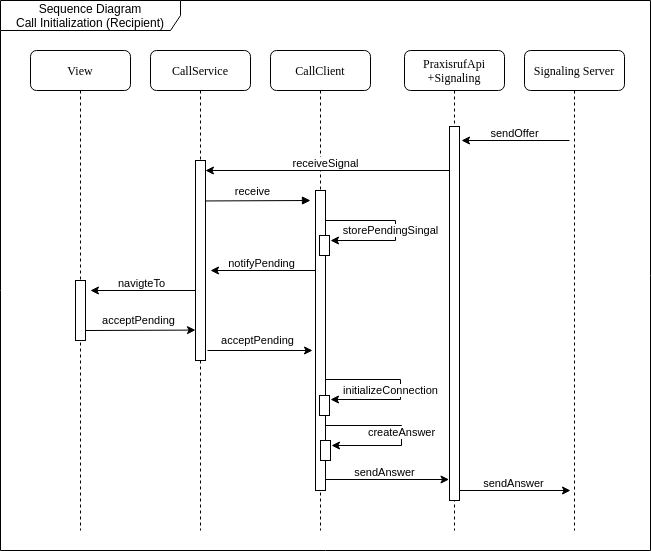
\includegraphics[width=\textwidth]{/home/joshua/FHNW/dev/IP6/IP6_Bachelorarbeit_Bericht_Cloudbasiertes_Praxisrufsystem/src/graphics/diagramms/Sequence_MobileClient_Receiver_Signaling.drawio.png}}
        \caption{Sequenzdiagramm - Initialisierung Sprachverbindung auf Empfängerseite }
    \end{minipage}
\end{figure}


Abbildung 7.23 zeigt den Ablauf bei Eingang eines Answer-Signals auf Empfängerseite.
Das versendete Signal wird über das Signaling Modul des Cloudservice an den Empfänger übermittelt.
Dieser empfängt das Signal über die Komponente PraxisrufApi+Signaling.
Diese gibt das Signal über die Methode onSignalReceived an den CallService weiter.
Der CallService aktiviert die Ansicht für aktive Anrufe und leitet das Signal an den CallClient weiter.
Der CallClient initialisiert die Peer-To-Peer Verbindung und erstellt ein Answer-Signal zur Bestätigung.
Dieses Signal wird wiederum über den CallService zum PraxisrufApi+Signaling weiter zum Cloudservice versendet.


\subsubsection{Netzwerkvoraussetzungen}

Praxisruf ist darauf ausgelegt innerhalb von Arztpraxen verwendet zu werden.
Dabei wird pro Zimmer ein Gerät installiert, welches als Endpunkt für das System dient~\cite{aufgabenstellung}.
Damit werden alle Endgeräte innerhalb derselben Praxis betrieben.
Dies erlaubt es, die Geräte über ein lokales Netzwerk zu verbinden.
Ist diese Voraussetzung gegeben, kann der Verbindungsaufbau vereinfacht werden.
Da die Geräte direkt im lokalen Netzwerk kommunizieren können, ist es nicht nötig, die Protokolle STUN oder TURN zu verwenden.
Damit wird es möglich auf den Betrieb eines ICE Servers zu verzichten.
Die Geräte können ICE Kandidaten für direkte Kommunikation im lokalen Netzwerk austauschen.

Die Integration von WebRTC in der iOS App wird unter der Voraussetzung umgesetzt, dass alle beteiligten Geräte im selben Netzwerk betrieben werden.
Dies vereinfacht den Aufbau von Verbindungen und erlaubt es, neben der Signaling Instanz keine weitere Infrastruktur betreiben zu müssen.
Sprachverbindungen mit Praxisruf sind deshalb nur möglich, wenn die beteiligten Geräte im selben lokalen Netzwerk betrieben werden.
Das Versenden und Empfangen von Benachrichtigungen funktioniert wie im Vorgängerprojekt auch ausserhalb des lokalen Netzwerkes.
Damit können auch für Empfänger, die nicht im lokalen Netzwerk sind, über verpasste Anrufe mit Benachrichtigungen informiert werden.

\clearpage

\subsection{Zusammenfassung}

\subsubsection{Mobile Client}

\textbf{TODO: } Add Views
\textbf{TODO: } Add Model
\begin{figure}[h]
    \centering
    \begin{minipage}[b]{0.92\textwidth}
        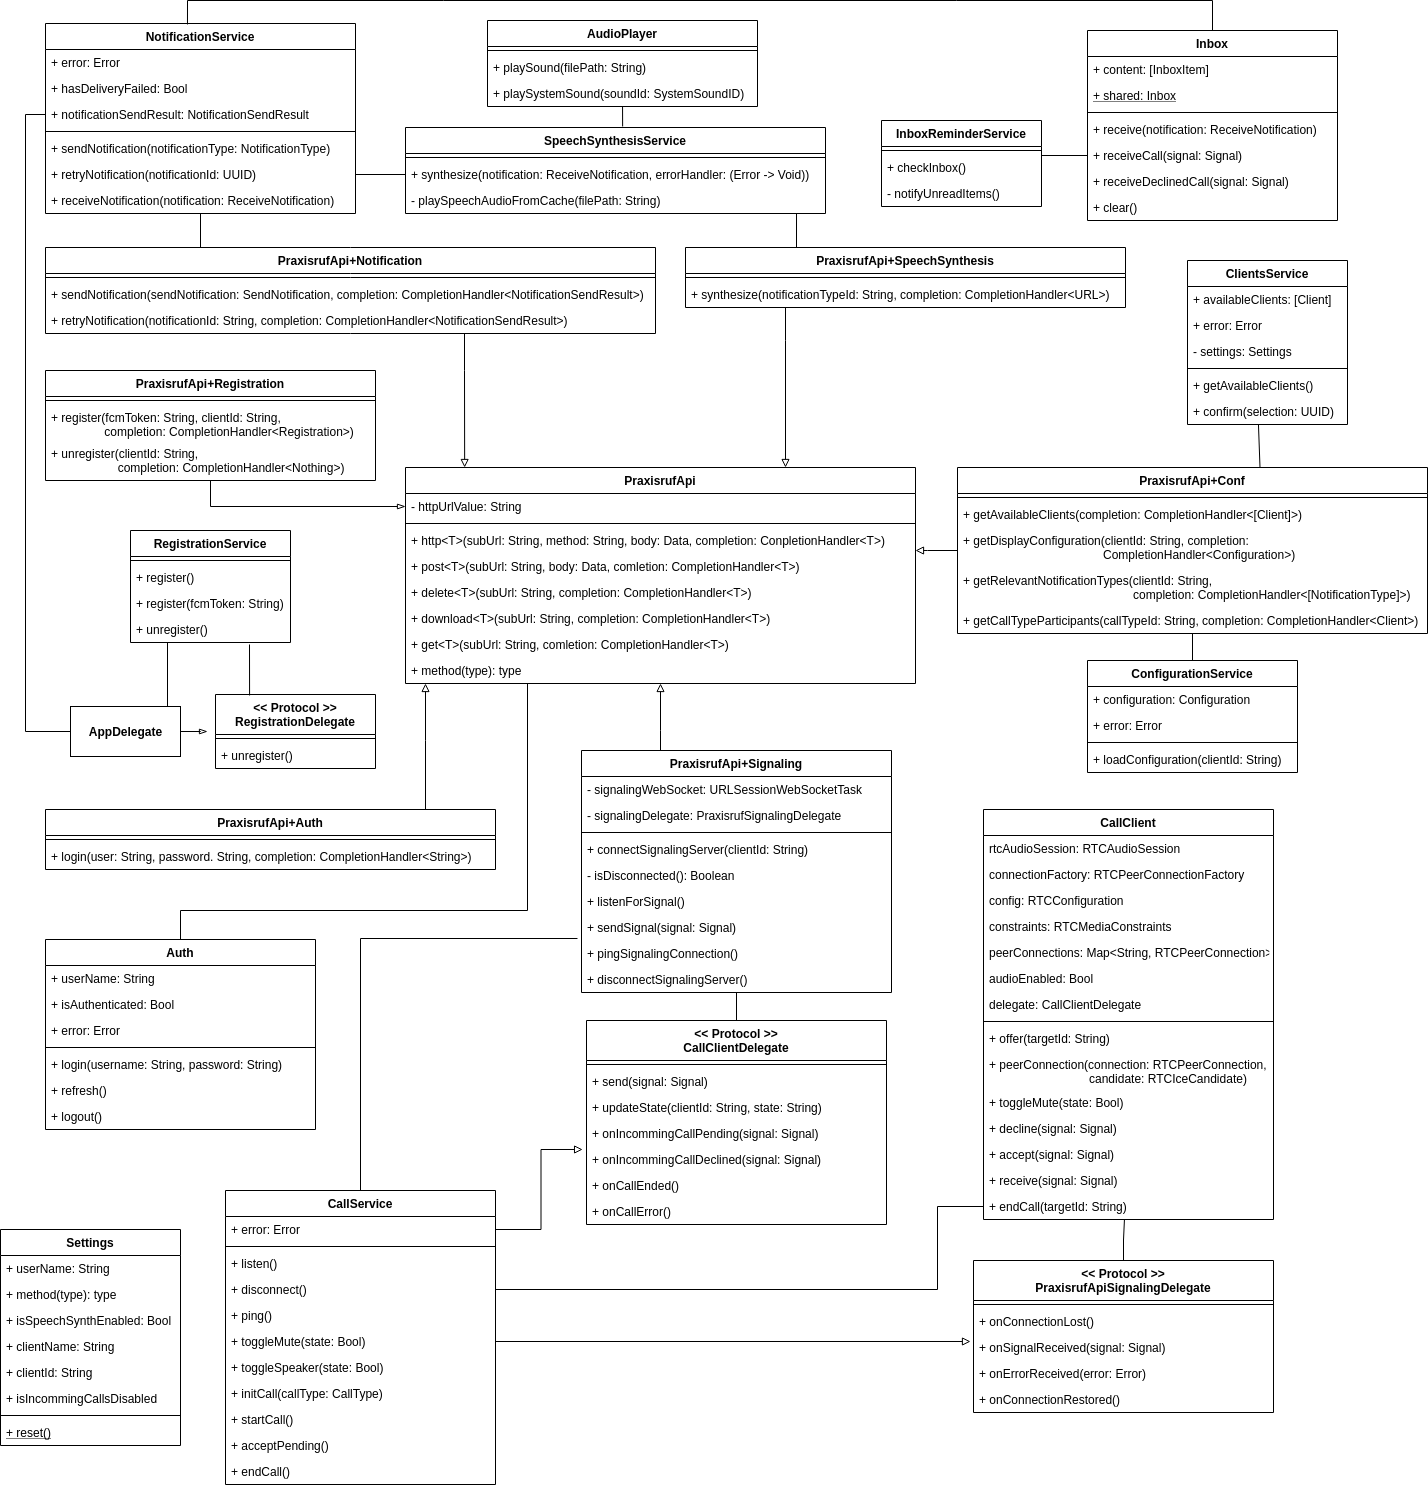
\includegraphics[width=\textwidth]{/home/joshua/FHNW/dev/IP6/IP6_Bachelorarbeit_Bericht_Cloudbasiertes_Praxisrufsystem/src/graphics/diagramms/Class_Mobile_Client_Draft_V02}
        \caption{Klassendiagramm Modul SpeechSynthesis}
    \end{minipage}
\end{figure}
\clearpage

\clearpage

\subsubsection{Cloudservice Entity Relation Diagramm}

\begin{figure}[h]
    \centering
    \begin{minipage}[b]{0.9\textwidth}
        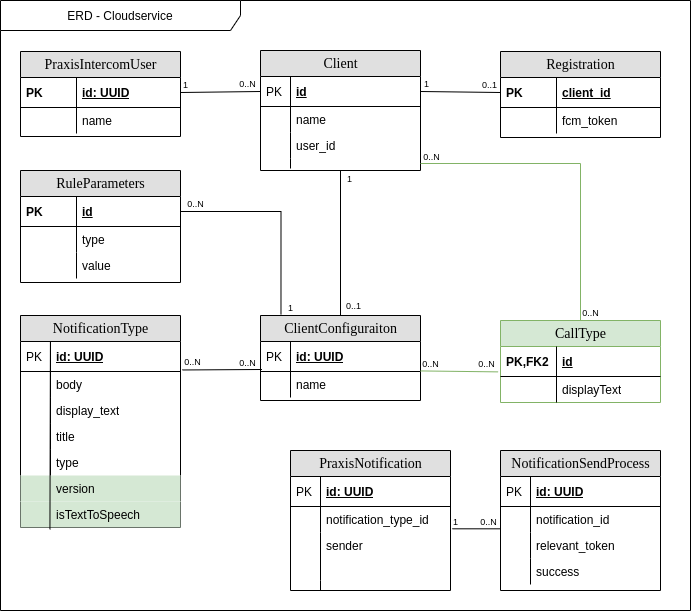
\includegraphics[width=\textwidth]{graphics/diagramms/erd_v02}
        \caption{Entitiy Relation Diagramm - Cloudservice}
    \end{minipage}
\end{figure}

\clearpage

\subsubsection{Cloudservice API}

Der Cloudservice wird um folgende Endpoints erweitert:

\begin{tabularx}{\textwidth}{|p{3cm}|l|l|X|X|}
    \hline
    \textbf{Aktion}                & \textbf{HTTP} & \textbf{Pfad}             & \textbf{Body}   & \textbf{Response} \\
    \hline
    Alle CallTypes laden    & GET          & /api/config/calltype       & - & [CallTypeDto]                 \\
    \hline
    CalLType laden        & GET        & /api/config/calltype/id       & -        & CallTypeDto                 \\
    \hline
    CallType erstellen & POST          & /api/config/calltypes & CallTypeDto & CallTypeDto \\
    \hline
    CallType aktualisieren & PUT          & /api/config/calltypes & CallTypeDto & CallTypeDto \\
    \hline
    CallType löschen & DELETE          & /api/config/calltypes/id & - & - \\
    \hline
    Mehrere CallTypes löschen & DELETE          & /api/config/calltypes/many/filter & - & - \\
    \hline
    Alle CallGroups laden    & GET          & /api/config/callgroup       & - & [CallGroupDto]                 \\
    \hline
    CallGroup laden        & GET        & /api/config/callgroup/id       & -        & CallGroupDto                 \\
    \hline
    CallGroup suchen        & GET        & /api/config/callgroup?callTypeId       & -        & [CallGroupDto]                 \\
    \hline
    CallGroup erstellen & POST          & /api/config/callgroup & CallGroupDto & CallGroupDto \\
    \hline
    CallGroup aktualisieren & PUT          & /api/config/callgroup & CallGroupDto & CallGroupDto \\
    \hline
    CallGroup löschen & DELETE          & /api/config/callgroup/id & - & - \\
    \hline
    Mehrere CallGroups löschen & DELETE          & /api/config/callgroup/many/filter & - & - \\
    \hline
    Sprachsynthese für notificationType        & GET        & /api/speech/id       & -        & MP3 Datei                 \\
    \hline
\end{tabularx}\label{tab:new-api-methods}

Zudem werden die bestehenden Endpoints zur Verwaltung von NotificationType und ClientConfiguration Daten erweitert.
Sodass neu CallTypes auf ClientConfigurations registriert werden können und das isTextToSpeech Flag auf NotificationTypes
gesetzt werden.

Letztlich wird ein neuer Websocket Endpoint unter /api/intercom/signaling veröffentlicht.

\clearpage


    \section{Umsetzung}

Dieses Kapitel beschreibt und evaluiert die erzielten Ergebnisse dieser Arbeit.
Zunächst wird eine Übersicht zum umgesetzten System gegeben.
Anschliessend werden die Resultate der durchgeführten Funktions- und Performancetests beschrieben.
Zum Schluss des Kapitels ein Fazit gezogen.

\subsection{Resultate}

Mit dieser Arbeit wurde das cloudbasiertes Praxisrufsystem aus dem Vorgängerprojekt ''IP5 Cloudbasiertes Praxisrufsystem'' erweitert.
Das erweiterte Rufsystem erlaubt es Benachrichtigungen zu Versenden und über Sprachverbindungen zu kommunizieren.
Es wurde eine native iOS App entwickelt, welche es erlaubt das Praxisrfusystem zu bedienen.
Diese App ersetzt den Mobile Client aus dem Vorgängerprojekt und unterstützt dabei alle Funktionen des alten Clients.

Mit Amazon Polly wurde ein Service für Sprachsynthese an das System angebunden.
Diese Anbindung wird verwendet, um bei Bedarf den Inhalt empfangener Benachrichtigungen automatisch vorlesen zu lassen.
Letztlich wurde WebRTC verwendet, um eine konfigurierbare Gegensprechanlage zu implementieren.
Diese erlaubt es über die iOS App Sprachverbindungen über das Praxisrufsystem aufzubauen.
Sowohl das Vorlesen von Benachrichtigungen, als auch die Gegensprechanlage sind über eine Weboberfläche konfigurierbar.

Die Meilensteine M01 bis M08 wurden erreicht.
Die Funktionalen Anforderungen an das System wurden umgesetzt.
Die bestehende Infrastruktur aus dem Vorgängerprojekt wurde für dieses Projekt weiterverwendet.
Die Komponenten Cloudservice, Messaging Service sowie Admin UI aus dem Vorgängerprojekt wurden weiterverwendet und wo nötig angepasst.
Umgesetzt wurden die Meilensteine mit folgenden User Stories:

\begin{itemize}
    \item U01 - Migration bestehender Funktion im Mobile Client
    \item U02 - Benachrichtigungen vorlesen
    \item U03 - Deaktivieren von Benachrichtung vorlesen
    \item U04 - Button für Sprachverbindung 1:1
    \item U05 - Button für Sprachverbindung 1:n
    \item U06 - Über Sprachverbindung in Echtzeit kommunizieren
    \item U07 - Nur relevante Buttons für Sprachverbindungen anzeigen
    \item U08 - Benachrichtigungston für eingehende Sprachverbindungen
    \item U09 - Empfangene und verpasste Sprachverbindungen in Inbox anzeigen
    \item U10 - Eingehende Sprachverbindungen automatisch öffnen
    \item U11 - Sprachverbindung beenden
    \item U13 - Vorlesen von Benachrichtigungen konfigurieren
    \item U14 - Buttons für Sprachverbindungen konfigurieren
    \item U15 - Konfiguration über Admin UI vornehmen
    \item U16 - Bestehende Infrastruktur übernehmen
    \item U17 - Weiterverwendung bestehender Komponenten
    \item U18 - Native iOS Applikation
    \item U19 - Für Externe Services Amazon Webservices verwenden
\end{itemize}


Der zu Beginn definierte Projektplan konnte grösstenteils eingehalten werden.
Setup- und Konzept-Phase wurden im geplanten Zeitraum abgeschlossen.
Während der Umsetzung ist es hingegen zu mehreren Verzögerungen gekommen.
Die Umsetzung und Testen der Gegensprechanlage hat deutlich mehr Zeit beansprucht, als eingeplant wurde.
Insbesondere die Integration und effiziente Verwendung von WebRTC im nativen iOS Client war anspruchsvoller als erwartet.
Dies ist einerseits auf die mangelhafte Dokumentation der verwendeten Bibliotheken zurückzuführen.
Andererseits wurde schlicht zu wenig Puffer für die Implementation eingeplant.
Die Verzögerungen während der Umsetzung hat dazu geführt, dass weniger Zeit als erhofft für Polishing und Erweiterungen aufgewendet werden konnten.
Dementsprechend konnte der Meilenstein M09 nicht vollständig erreicht werden.
Das entwickelte System hat in den Bereichen Stabilität und Benutzerfreundlichkeit noch Lücken.
Diese Werden in Kapitel 8.x beschrieben.

Der Meilenstein M10 betrifft Abschluss und Abgabe des Projektes.
Er ist mit dem Abschluss dieses Projektes erfüllt.

\subsubsection{Native iOS Applikation}

Dieses Kapitel beschreibt das umgesetzte cloudbasierte Praxisrufsystem anhand der Ansichten der iOS Applikation.
Sämtliche in diesem Kapitel dargestellten Ansichten wurden als Screenshots auf einem iPad 9. Generation erstellt.

\subsubsection*{Anmeldung und Konfiguration}

Der Mobile Client bietet eine einfaches Verfahren zur Anmeldung und Konfiguration.
In einem ersten Schritt gibt der Praxismitarbeitende Benutzername und Passwort ein.
Anschliessend kann er auf einer zweiten Ansicht, die gewünschte Zimmerkonfiguration wählen.
Benutzer und Zimmerkonfiguration werden dabei gespeichert.
Bis sich der Benutzer manuell abmeldet wird bei allen zukünftigen Starts der App die gespeicherte Kombination von Benutzer und Zimmerkonfiguration wiederverwendet.

\begin{figure}[h]
    \centering
    \begin{minipage}[b]{0.45\textwidth}
        \fbox{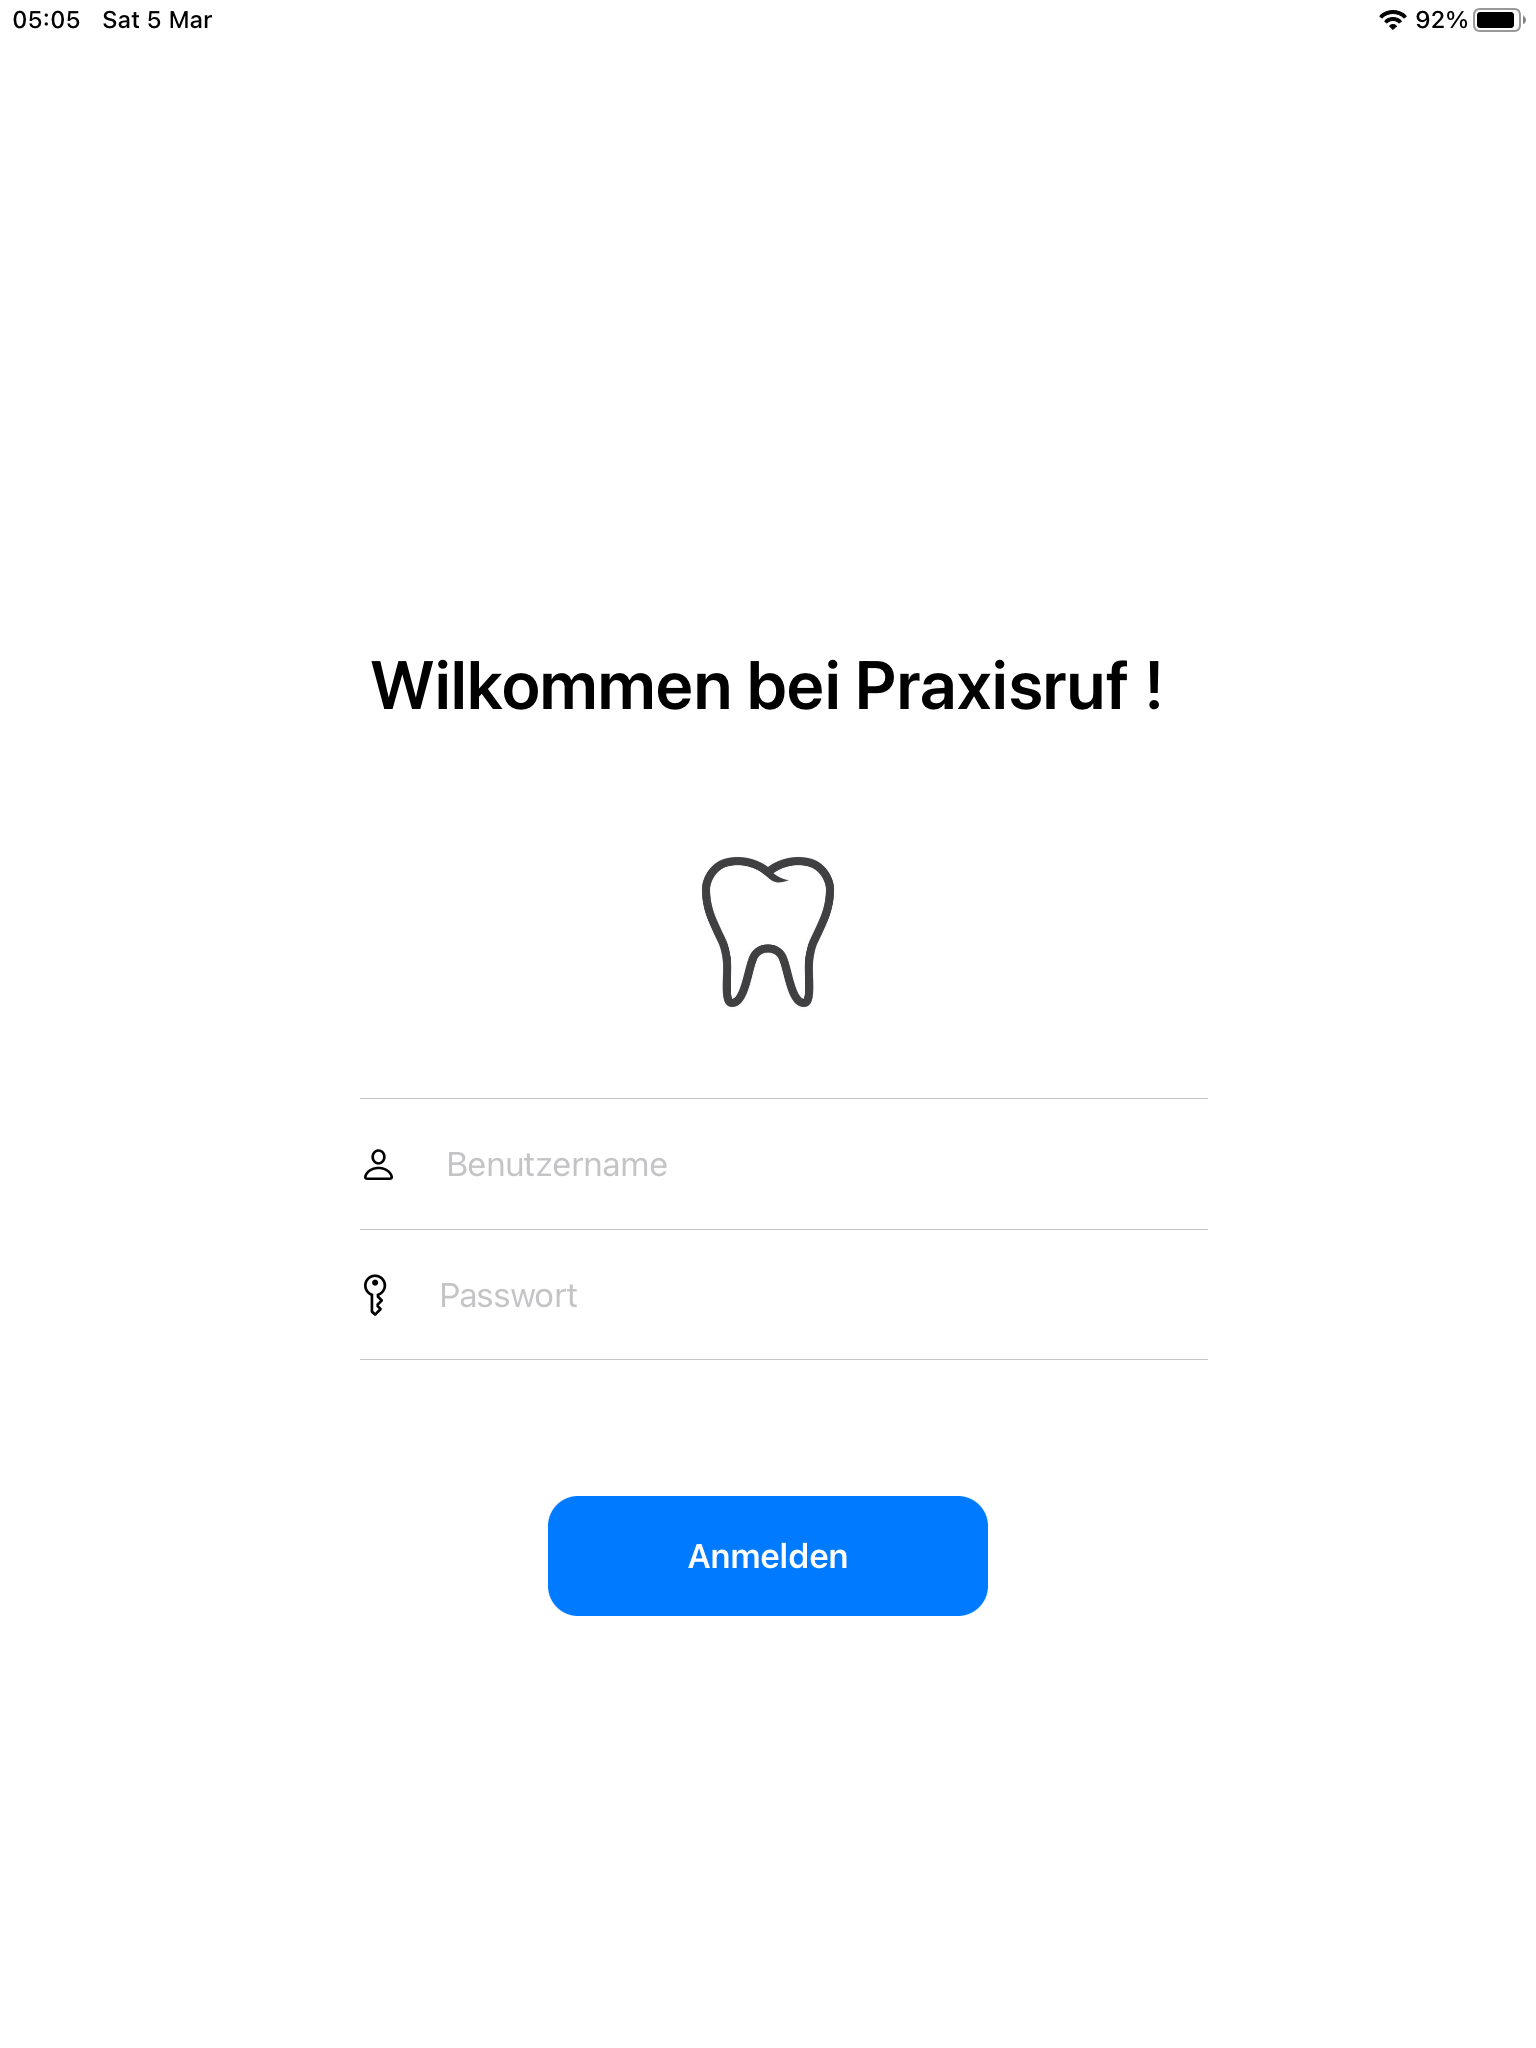
\includegraphics[width=\textwidth]{graphics/screenshots/app/login}}
        \caption{Ansicht Login}
    \end{minipage}
    \hfill
    \begin{minipage}[b]{0.45\textwidth}
        \fbox{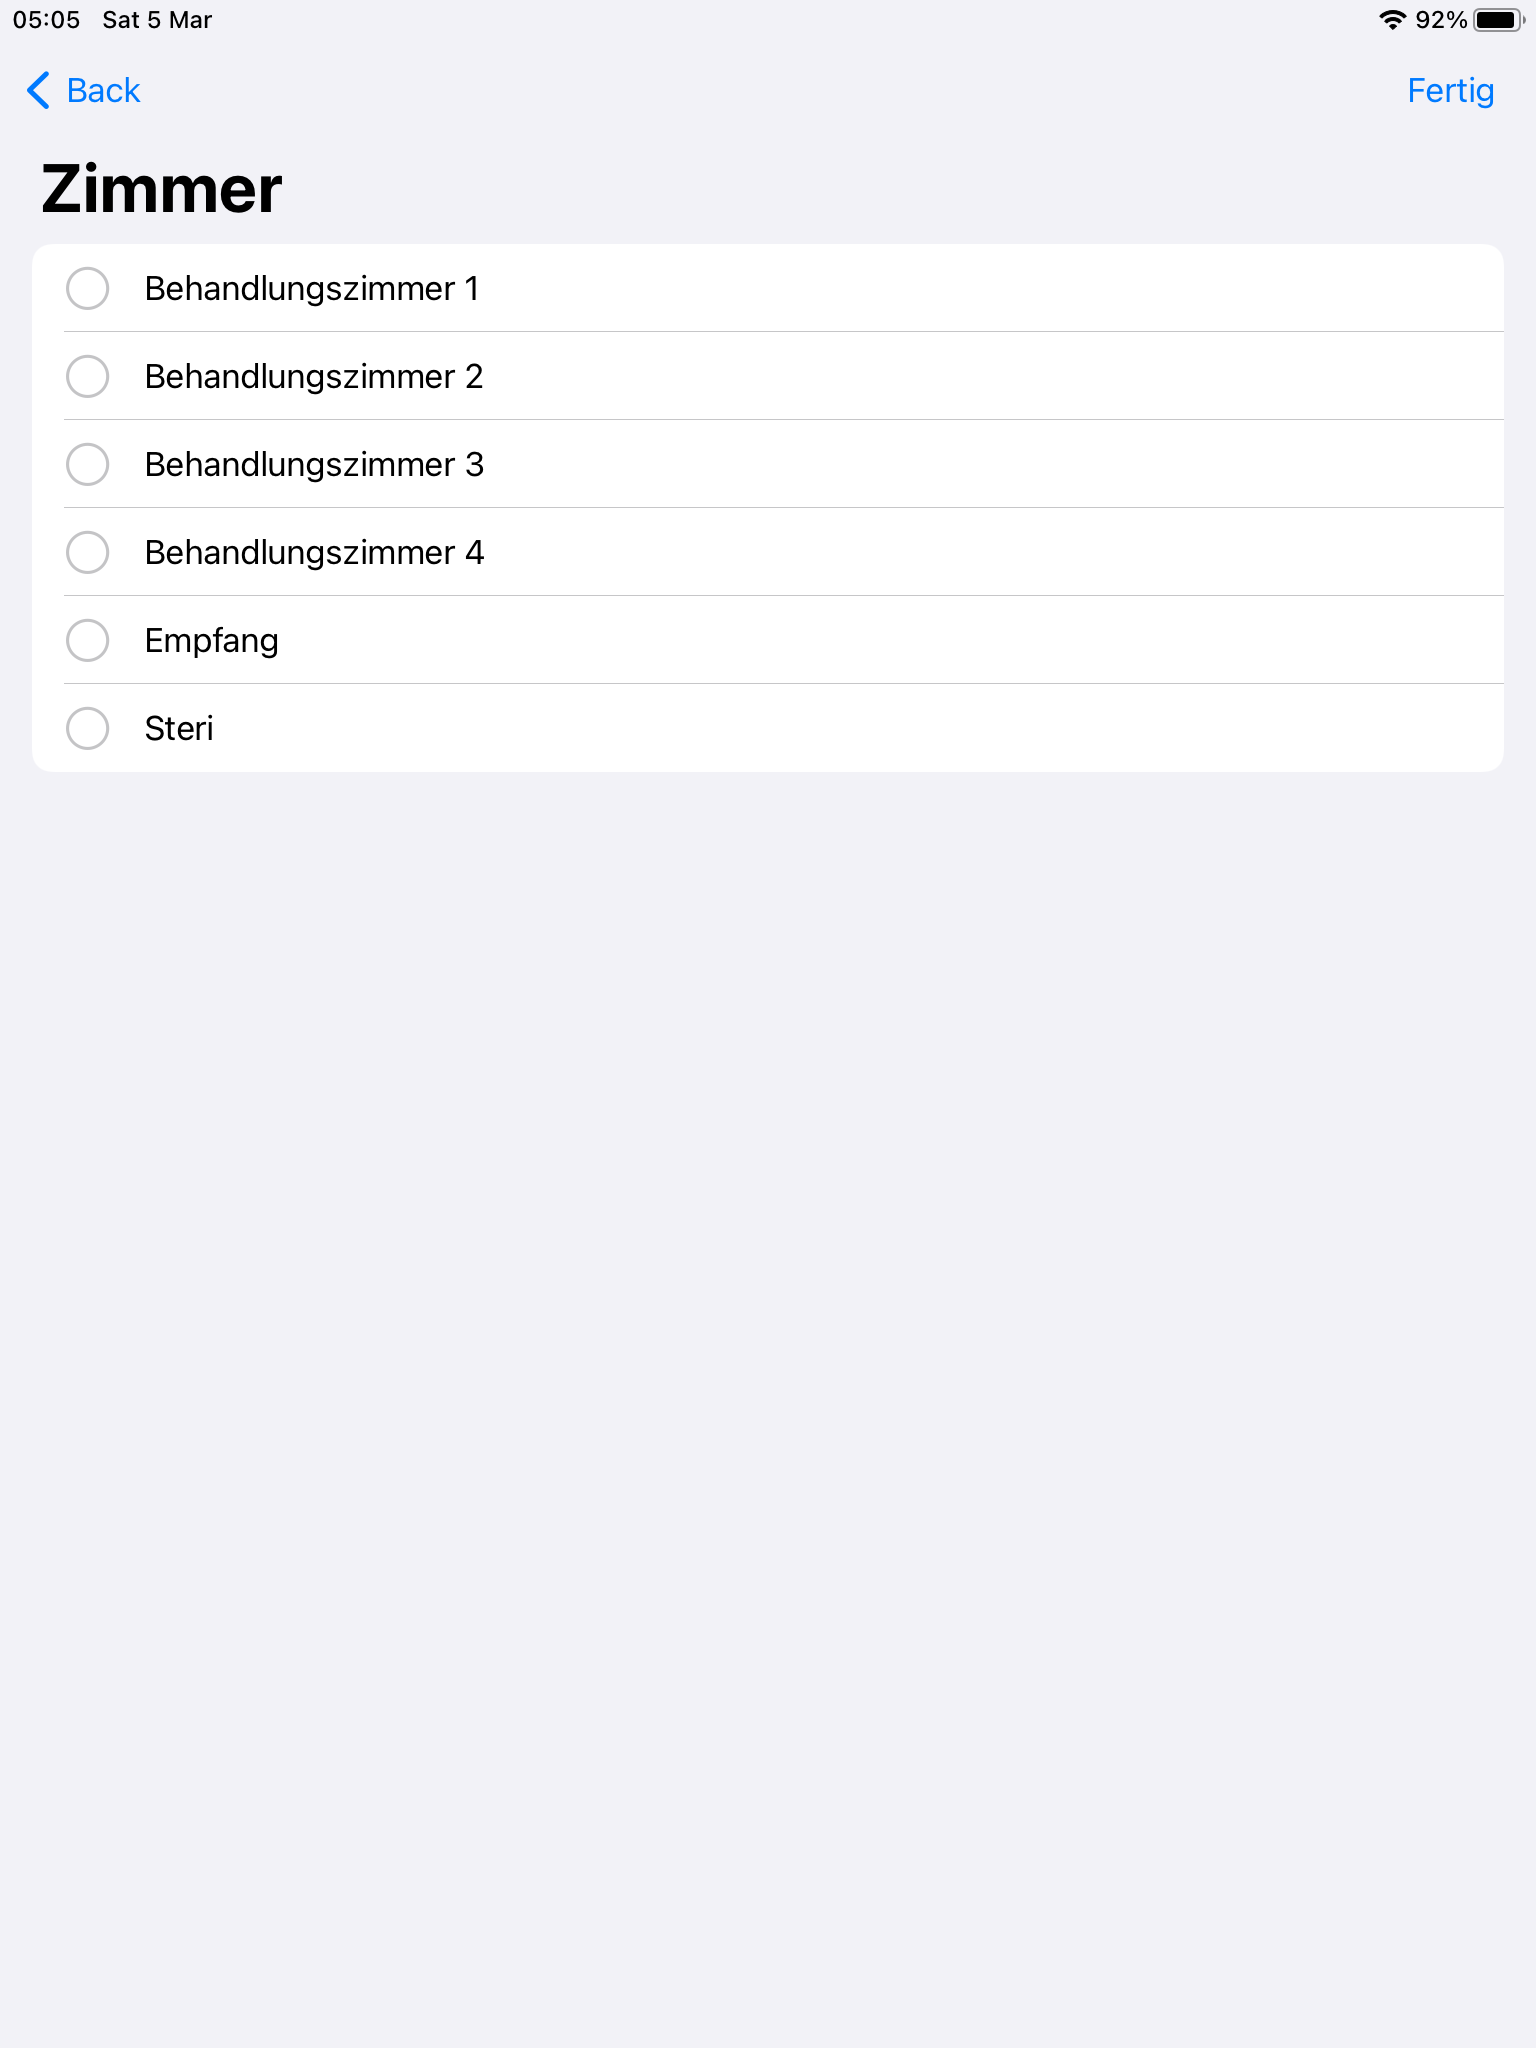
\includegraphics[width=\textwidth]{graphics/screenshots/app/client_select}}
        \caption{Ansicht Zimmerwahl }
    \end{minipage}

    \label{fig:MobileClient-Screens1}

\end{figure}

\clearpage

\subsubsection*{Startseite und Inbox}

Nach der Anmeldung und Konfigurationsauswahl wird der Benutzer auf die Hauptansicht der App weitergeleitet.
Über eine Navigationsleiste am unteren Bildschirmrand kann zwischen den Bereichen Home, Inbox und Einstellungen
Der Bereich Home ist in zwei Teile gegliedert und beinhaltet Buttons über welche Benachrichtigungen versendet und Sprachverbindungen gestartet werden können.
Welche Buttons zur Verfügung stehen werden durch die gewählte Zimmerkonfiguration vorgegeben und wurden im Vorfeld vom Praxisadministrator konfiguriert.
Der Bereich Inbox zeigt eine Liste von empfangenen Benachrichtigungen sowie verpassten und vergangenen Anrufen.
Einträge in dieser Liste können durch eine Wischgeste (Swipe right) entfernt werden.

\begin{figure}[h]
    \centering
    \begin{minipage}[b]{0.45\textwidth}
        \fbox{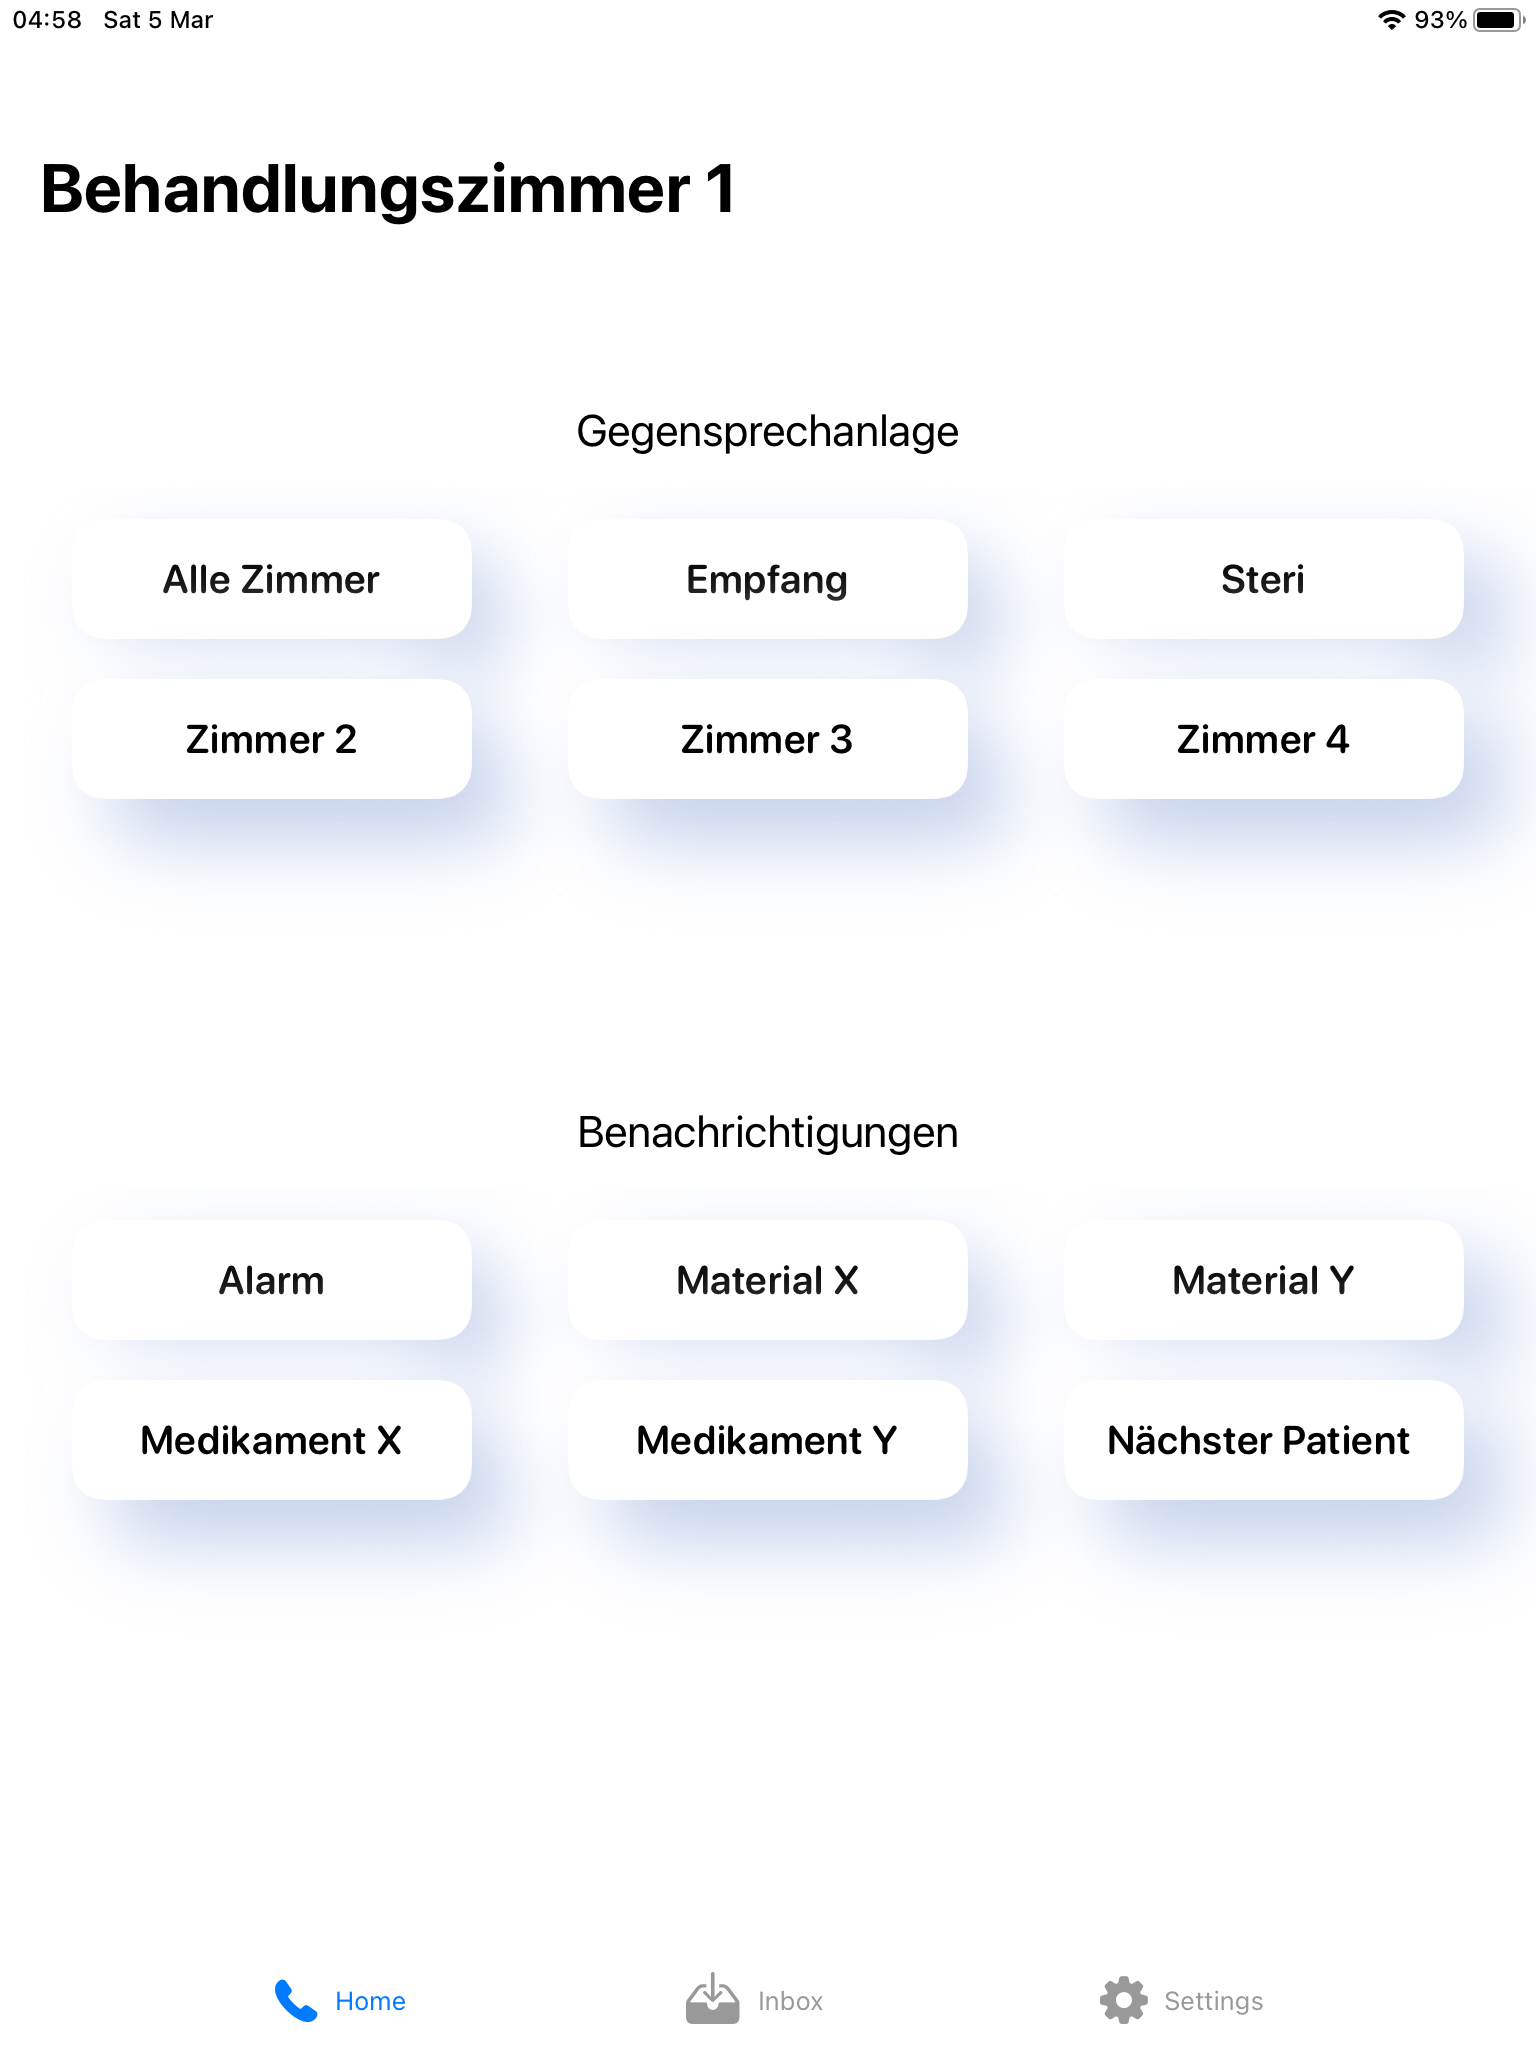
\includegraphics[width=\textwidth]{graphics/screenshots/app/home}}
        \caption{Ansicht Home}
    \end{minipage}
    \hfill
    \begin{minipage}[b]{0.45\textwidth}
        \fbox{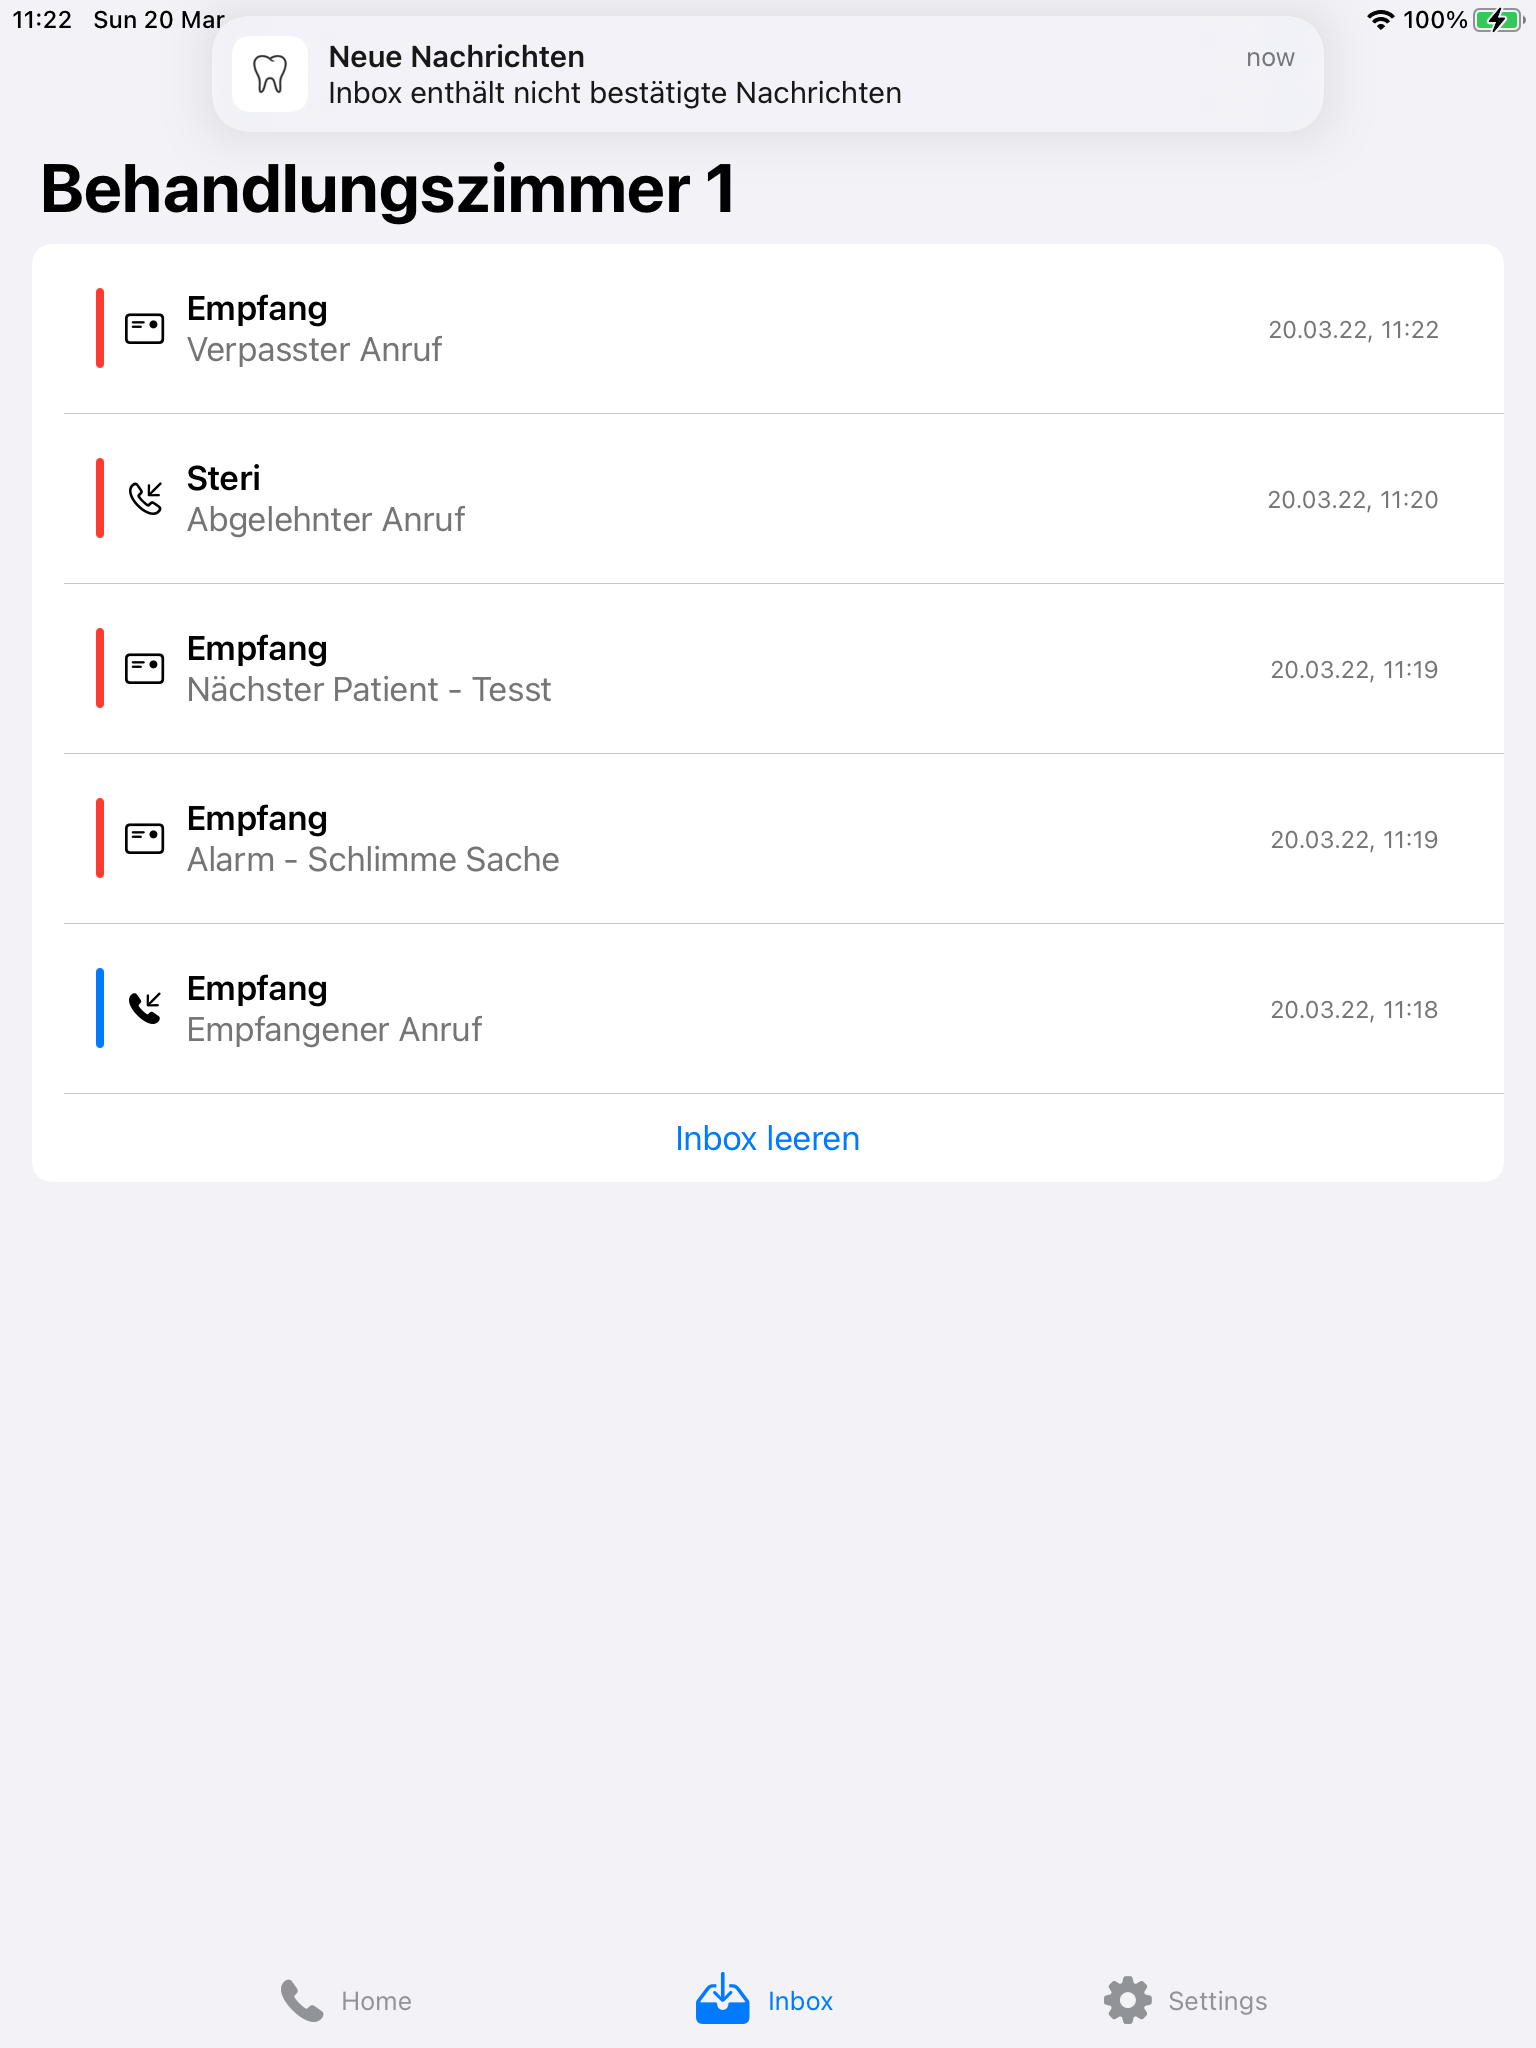
\includegraphics[width=\textwidth]{graphics/screenshots/app/inbox}}
        \caption{Ansicht Inbox}
    \end{minipage}
    \label{fig:MobileClient-Screens2}
\end{figure}

\clearpage

\subsubsection*{Einstellungen und Aktive Anrufe}

Im Bereich Einstellungen werden Informationen zur gewählten Zimmerkonfiguration und dem angemeldeten Benutzer angezeigt.
Weiter können lokale Einstellungen vorgenommen werden.
Das Vorlesen von empfangenen Benachrichtigungen sowie das Empfangen von Anrufen kann hier deaktiviert werden.
Über einen Button kann der Benutzer sich zudem von der App abmelden.

\begin{figure}[h]
    \centering
    \begin{minipage}[b]{0.45\textwidth}
        \fbox{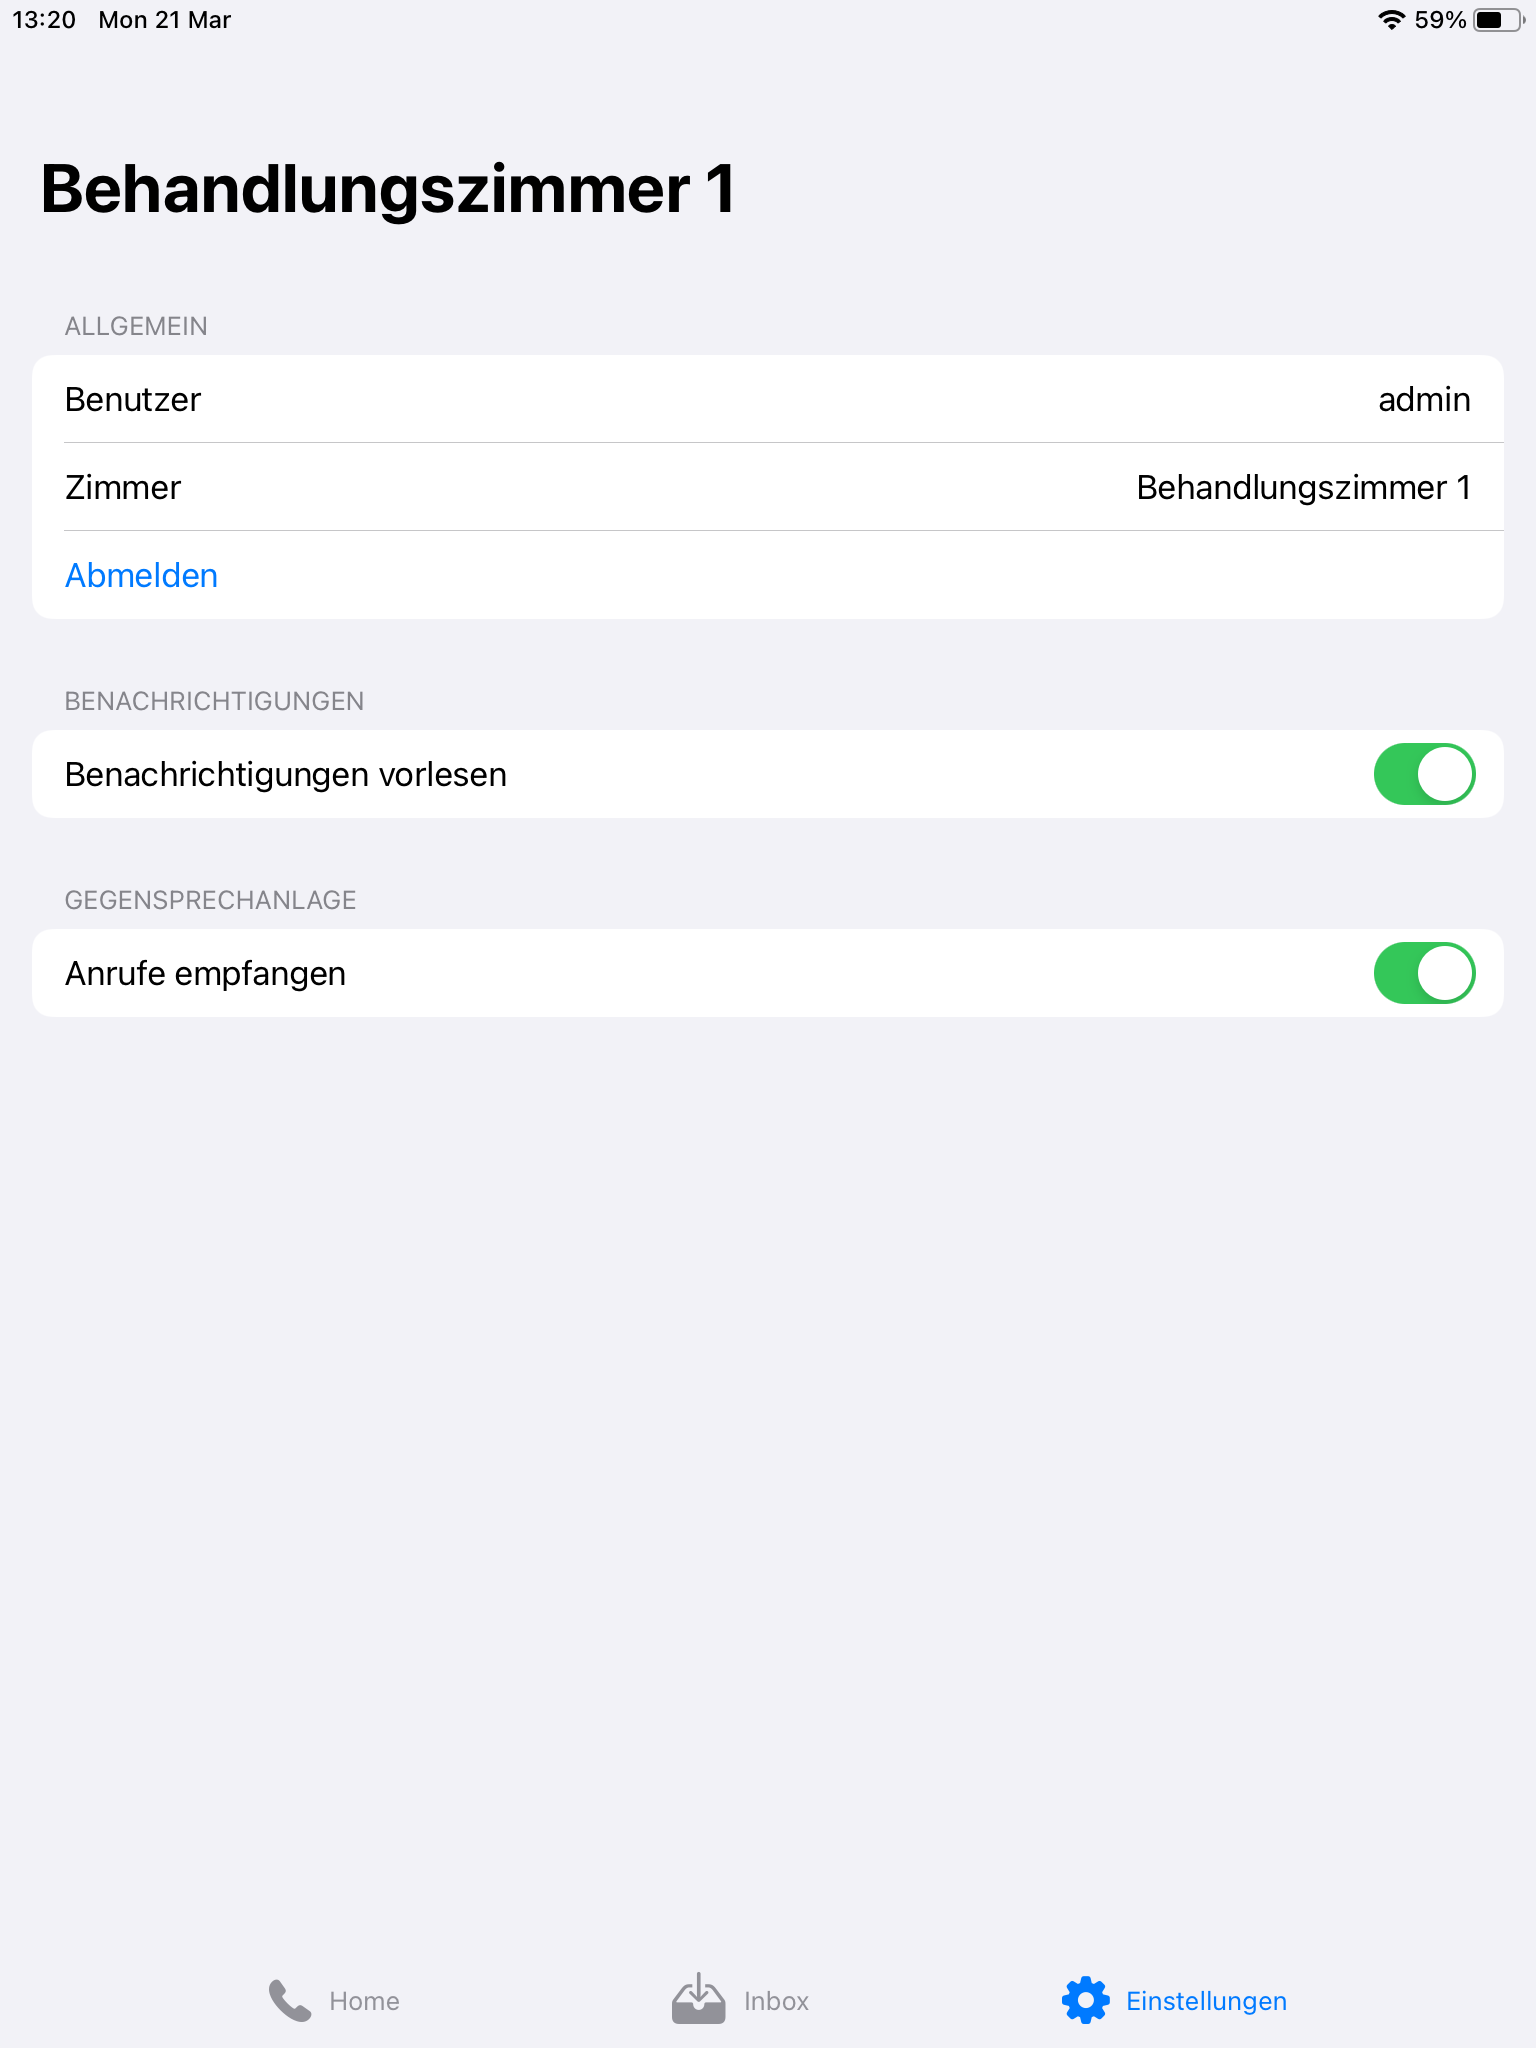
\includegraphics[width=\textwidth]{graphics/screenshots/app/settings}}
        \caption{Ansicht Settings}
    \end{minipage}
    \hfill
    \begin{minipage}[b]{0.45\textwidth}
        \fbox{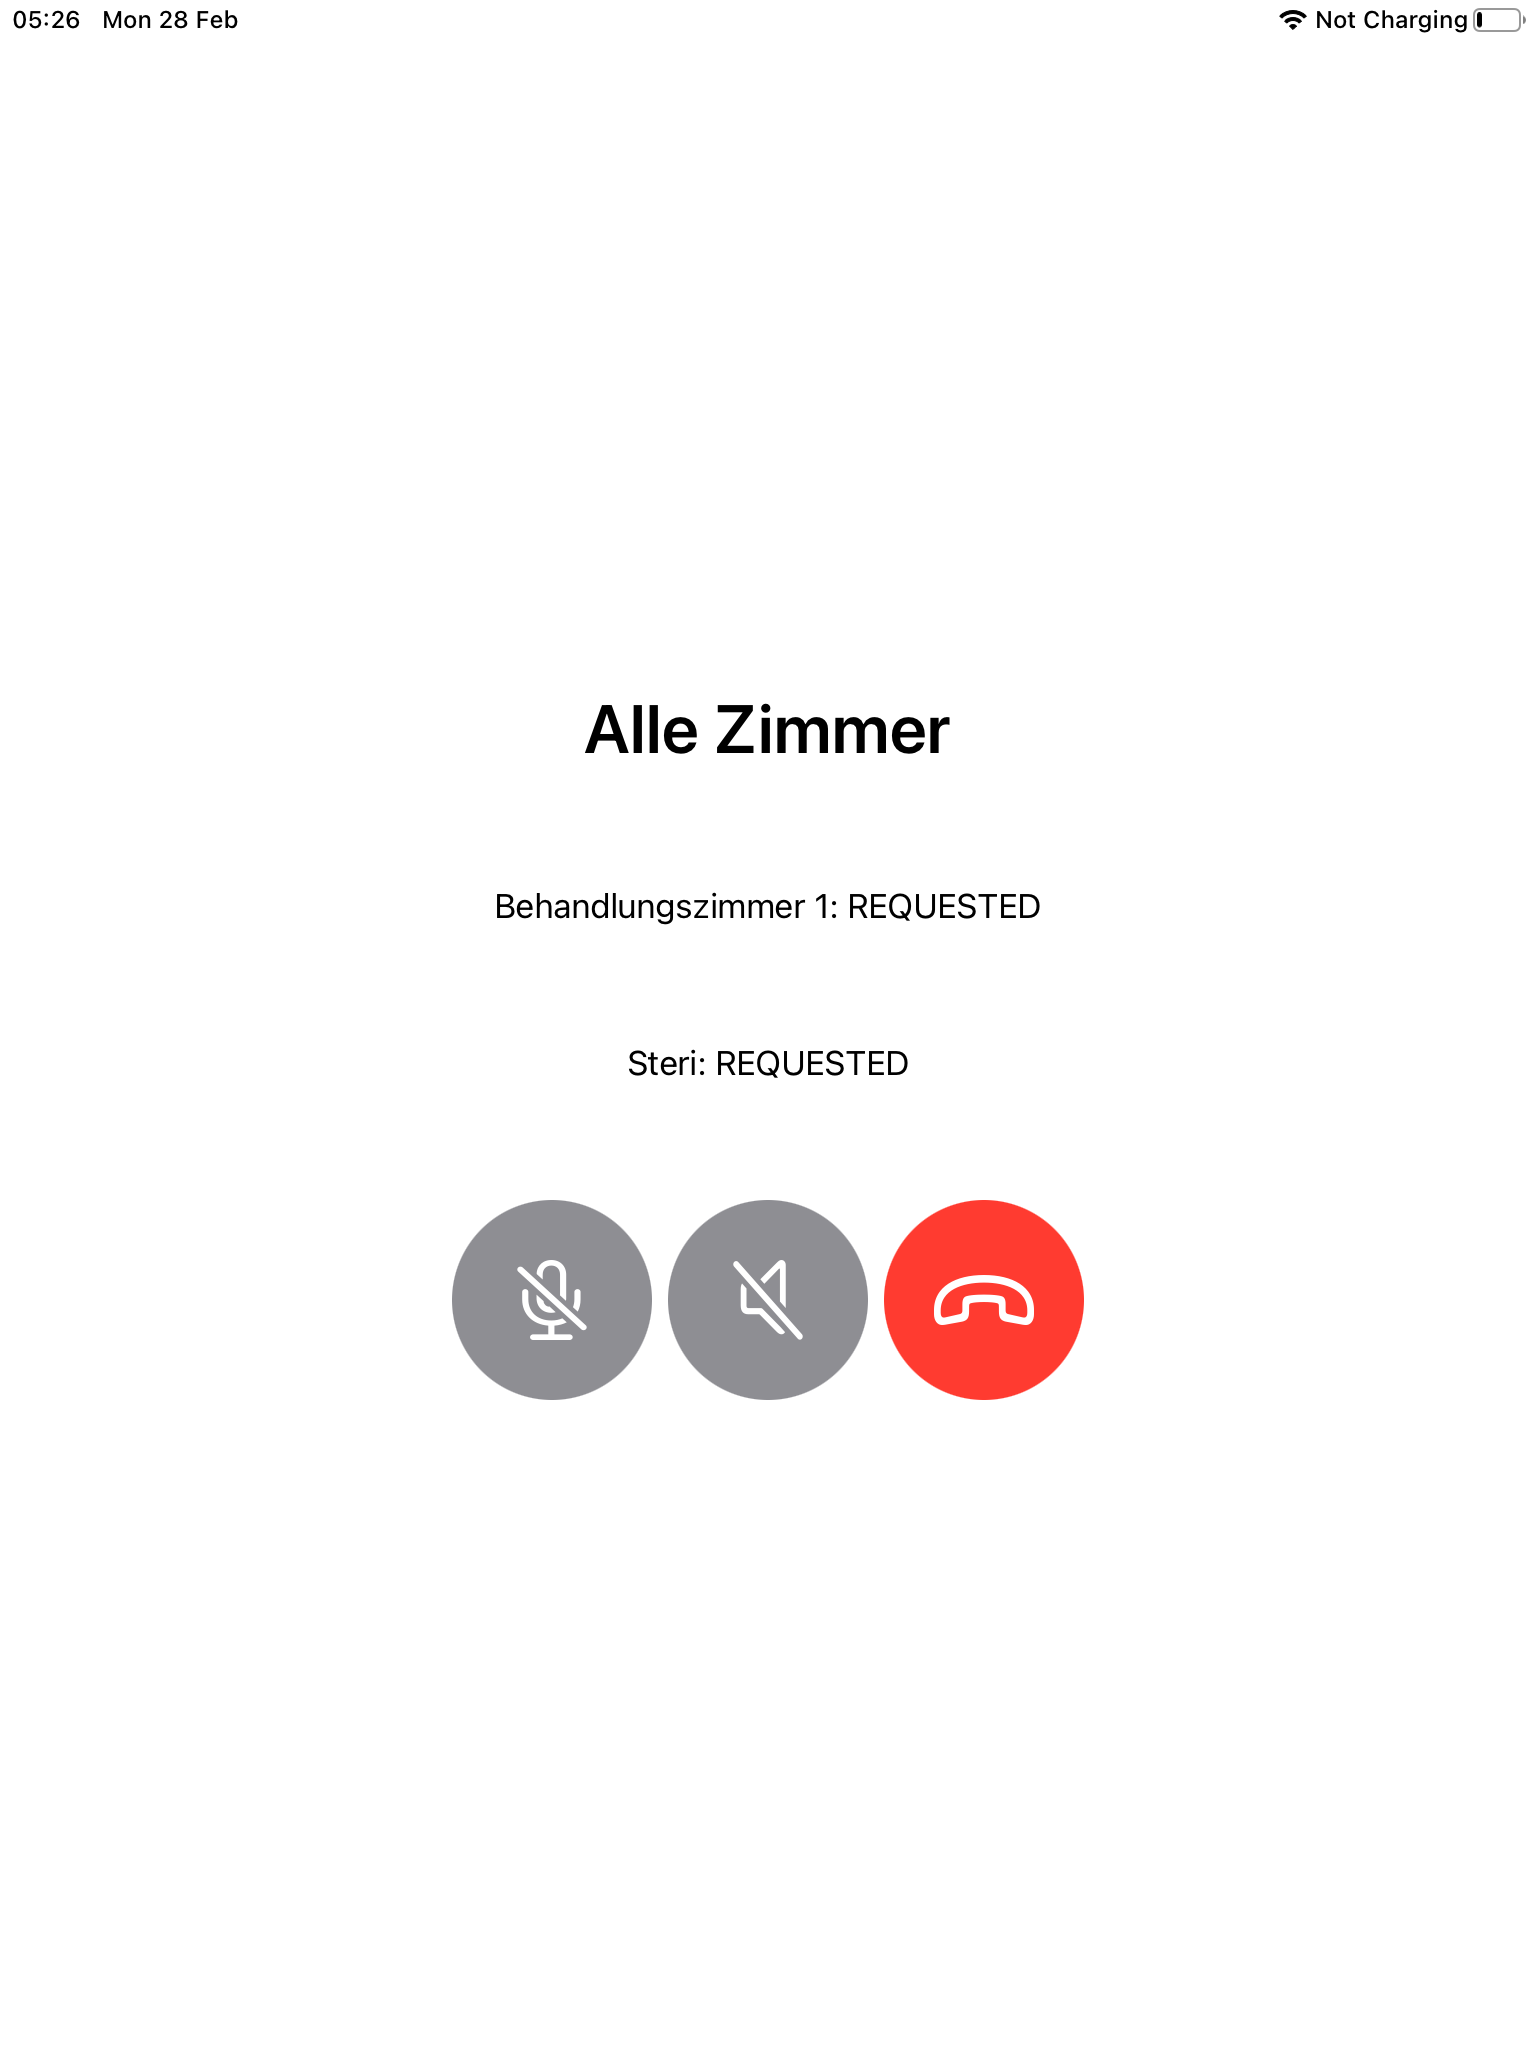
\includegraphics[width=\textwidth]{graphics/screenshots/app/call}}
        \caption{Ansicht Aktiver Anruf}
    \end{minipage}
    \label{fig:MobileClient-Screens3}
\end{figure}

Die Ansicht ''Aktive Anruf'' wird angezeigt, nachdem ein Anruf gestartet wurde.
Entweder, der Anruf durch antippen des Buttons in der Home Ansicht gestartet wurde oder weil ein Anruf von einem anderen Client empfangen wird.
In dieser Ansicht wird der Titel des gestarteten Anrufes bzw. Name des Zimmer des Gesprächspartners angezeigt.
Wenn mehr als ein Gesprächspartner am Anruf beteiligt ist, wird zudem eine Liste der Teilnehmer zusammen mit deren Verbindungsstatus angezeigt.
Allen Gesprächsteilnehmern stehen Buttons zur Stummschaltung des eigenen Lautsprechers und Microphons zur Verfügung.
Zudem können alle Gesprächsteilehmmer die Unterhaltung durch den roten Auflegen Button beenden.

\clearpage

\subsubsection*{Hintergrundbenachrichtigungen und Fehlerhandling}

Benachrichtigungen können mit dem cloudbasierten Praxisrufsystem im Hintergrund empfangen werden.
Im Hintergrund empfangene Benachrichtigungen erscheinen als Push Benachrichtigungen auf dem Home Screen des iPads.
Anrufe über die Gegensprechanlage können nur empfangen werden, wenn die Applikation geöffnet ist.
Ist die App minimiert oder beendet, ist der jeweilige Client für Gespräche nicht verfügbar.
Ein nicht verfügbarer Client wird über Hintergrundbenachrichtigungen auf verpasste Anrufe hingewiesen.

\begin{figure}[h]
    \centering
    \begin{minipage}[b]{0.45\textwidth}
        \fbox{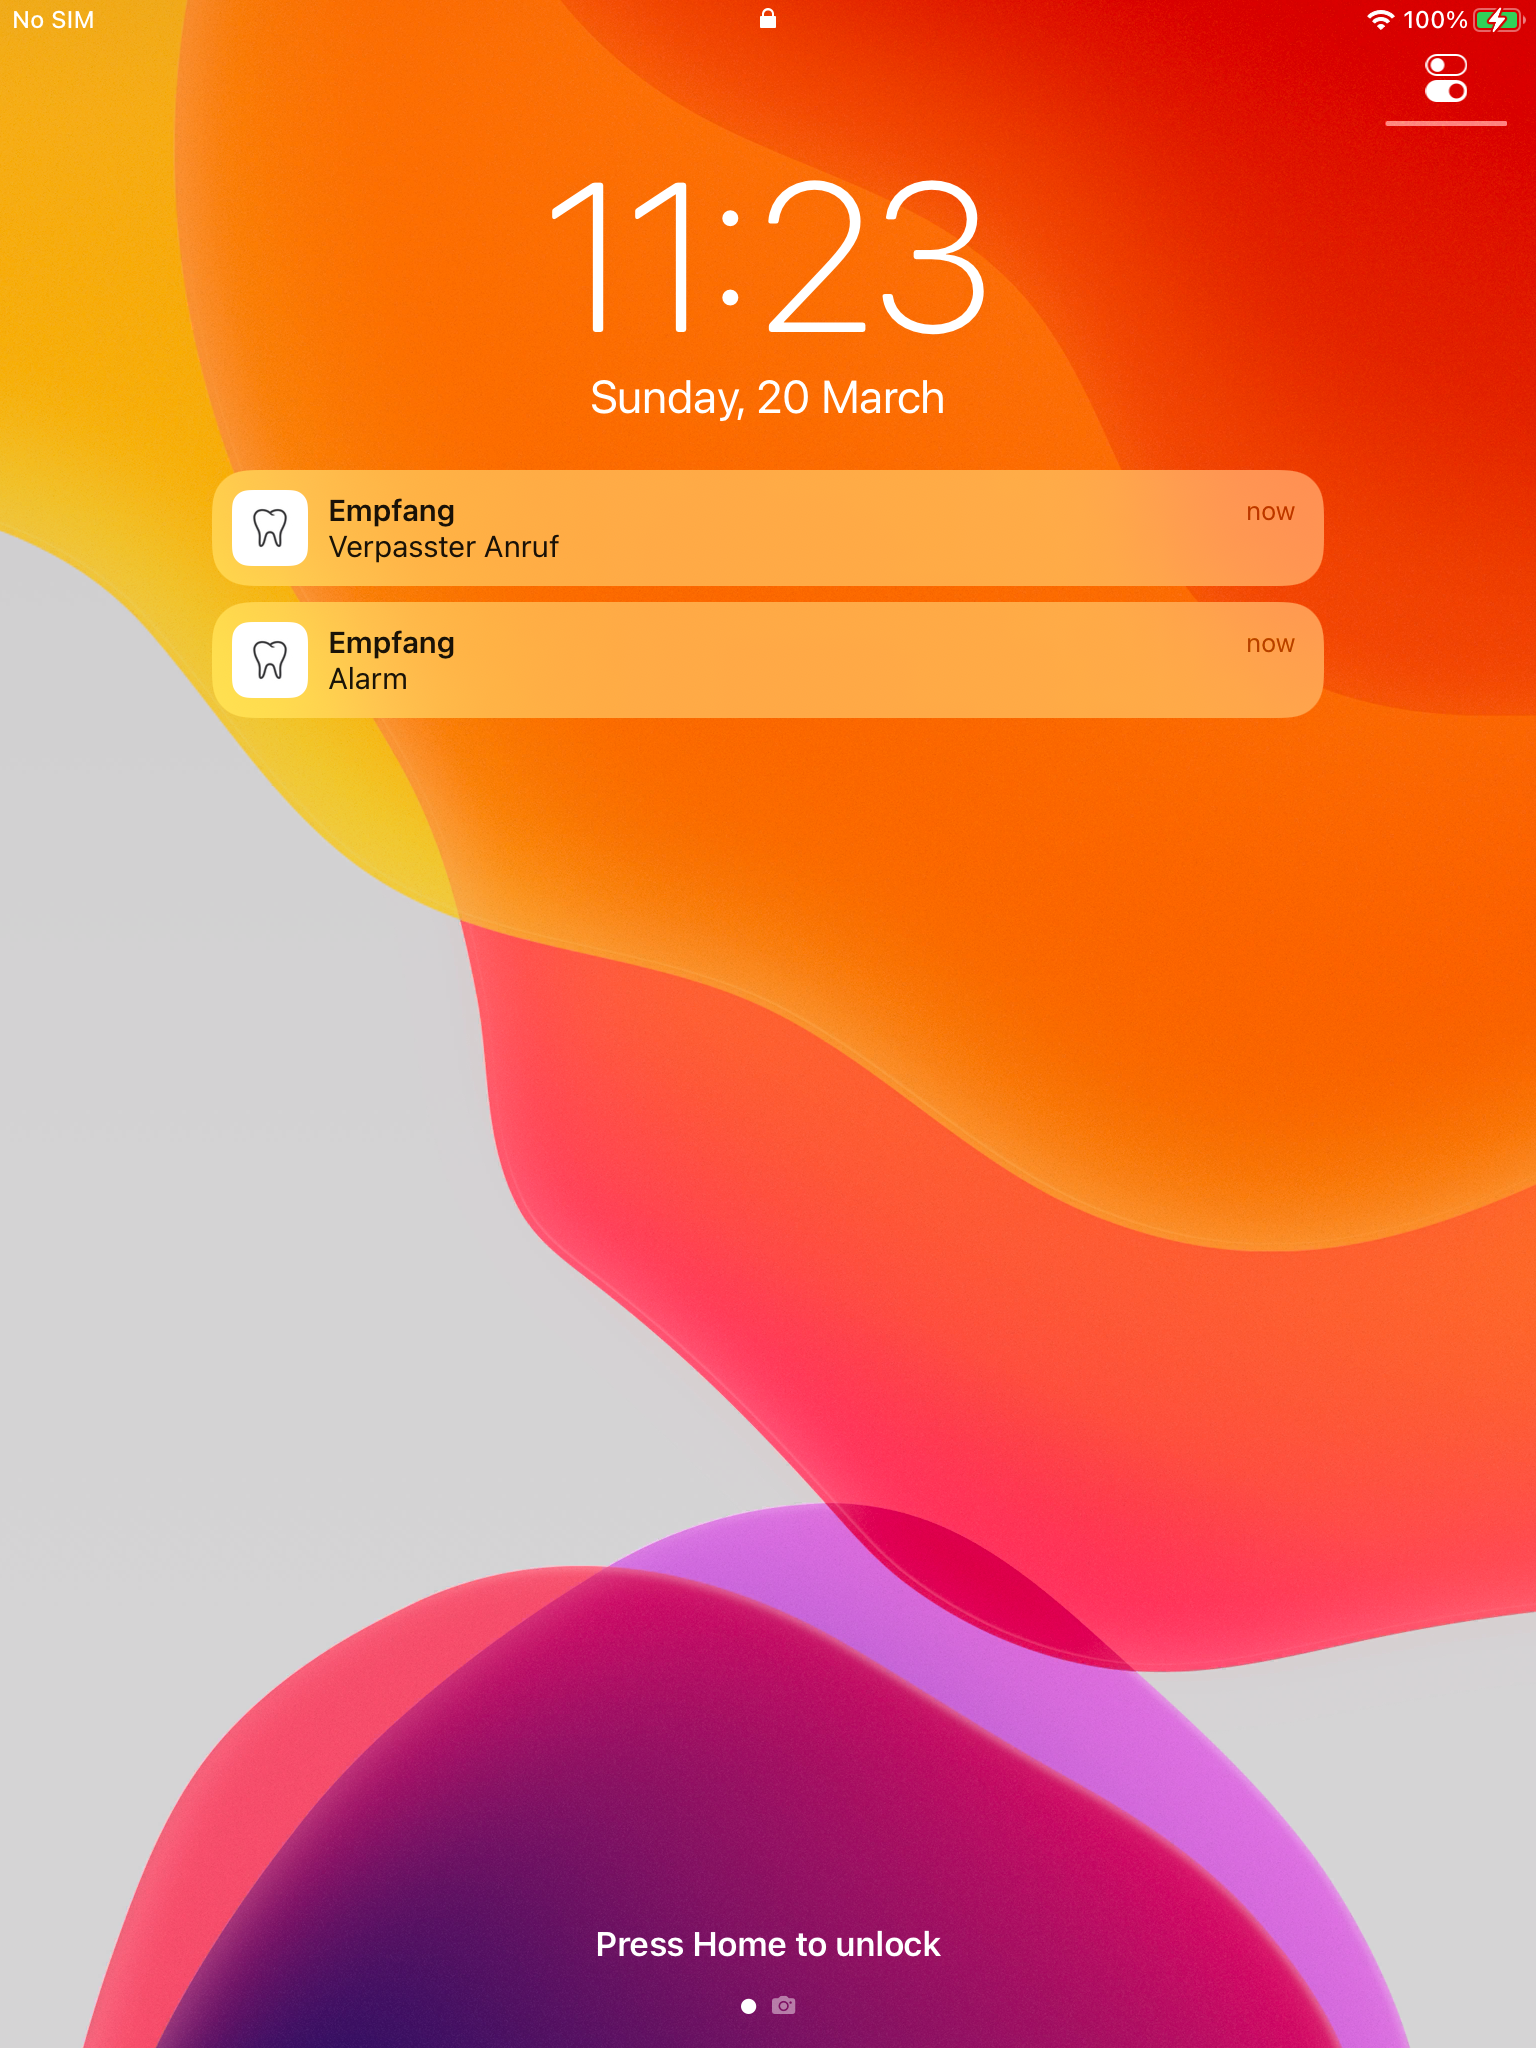
\includegraphics[width=\textwidth]{graphics/screenshots/app/background_notification}}
        \caption{Hintergrund Benachrichtigung}
    \end{minipage}
    \hfill
    \begin{minipage}[b]{0.45\textwidth}
        \fbox{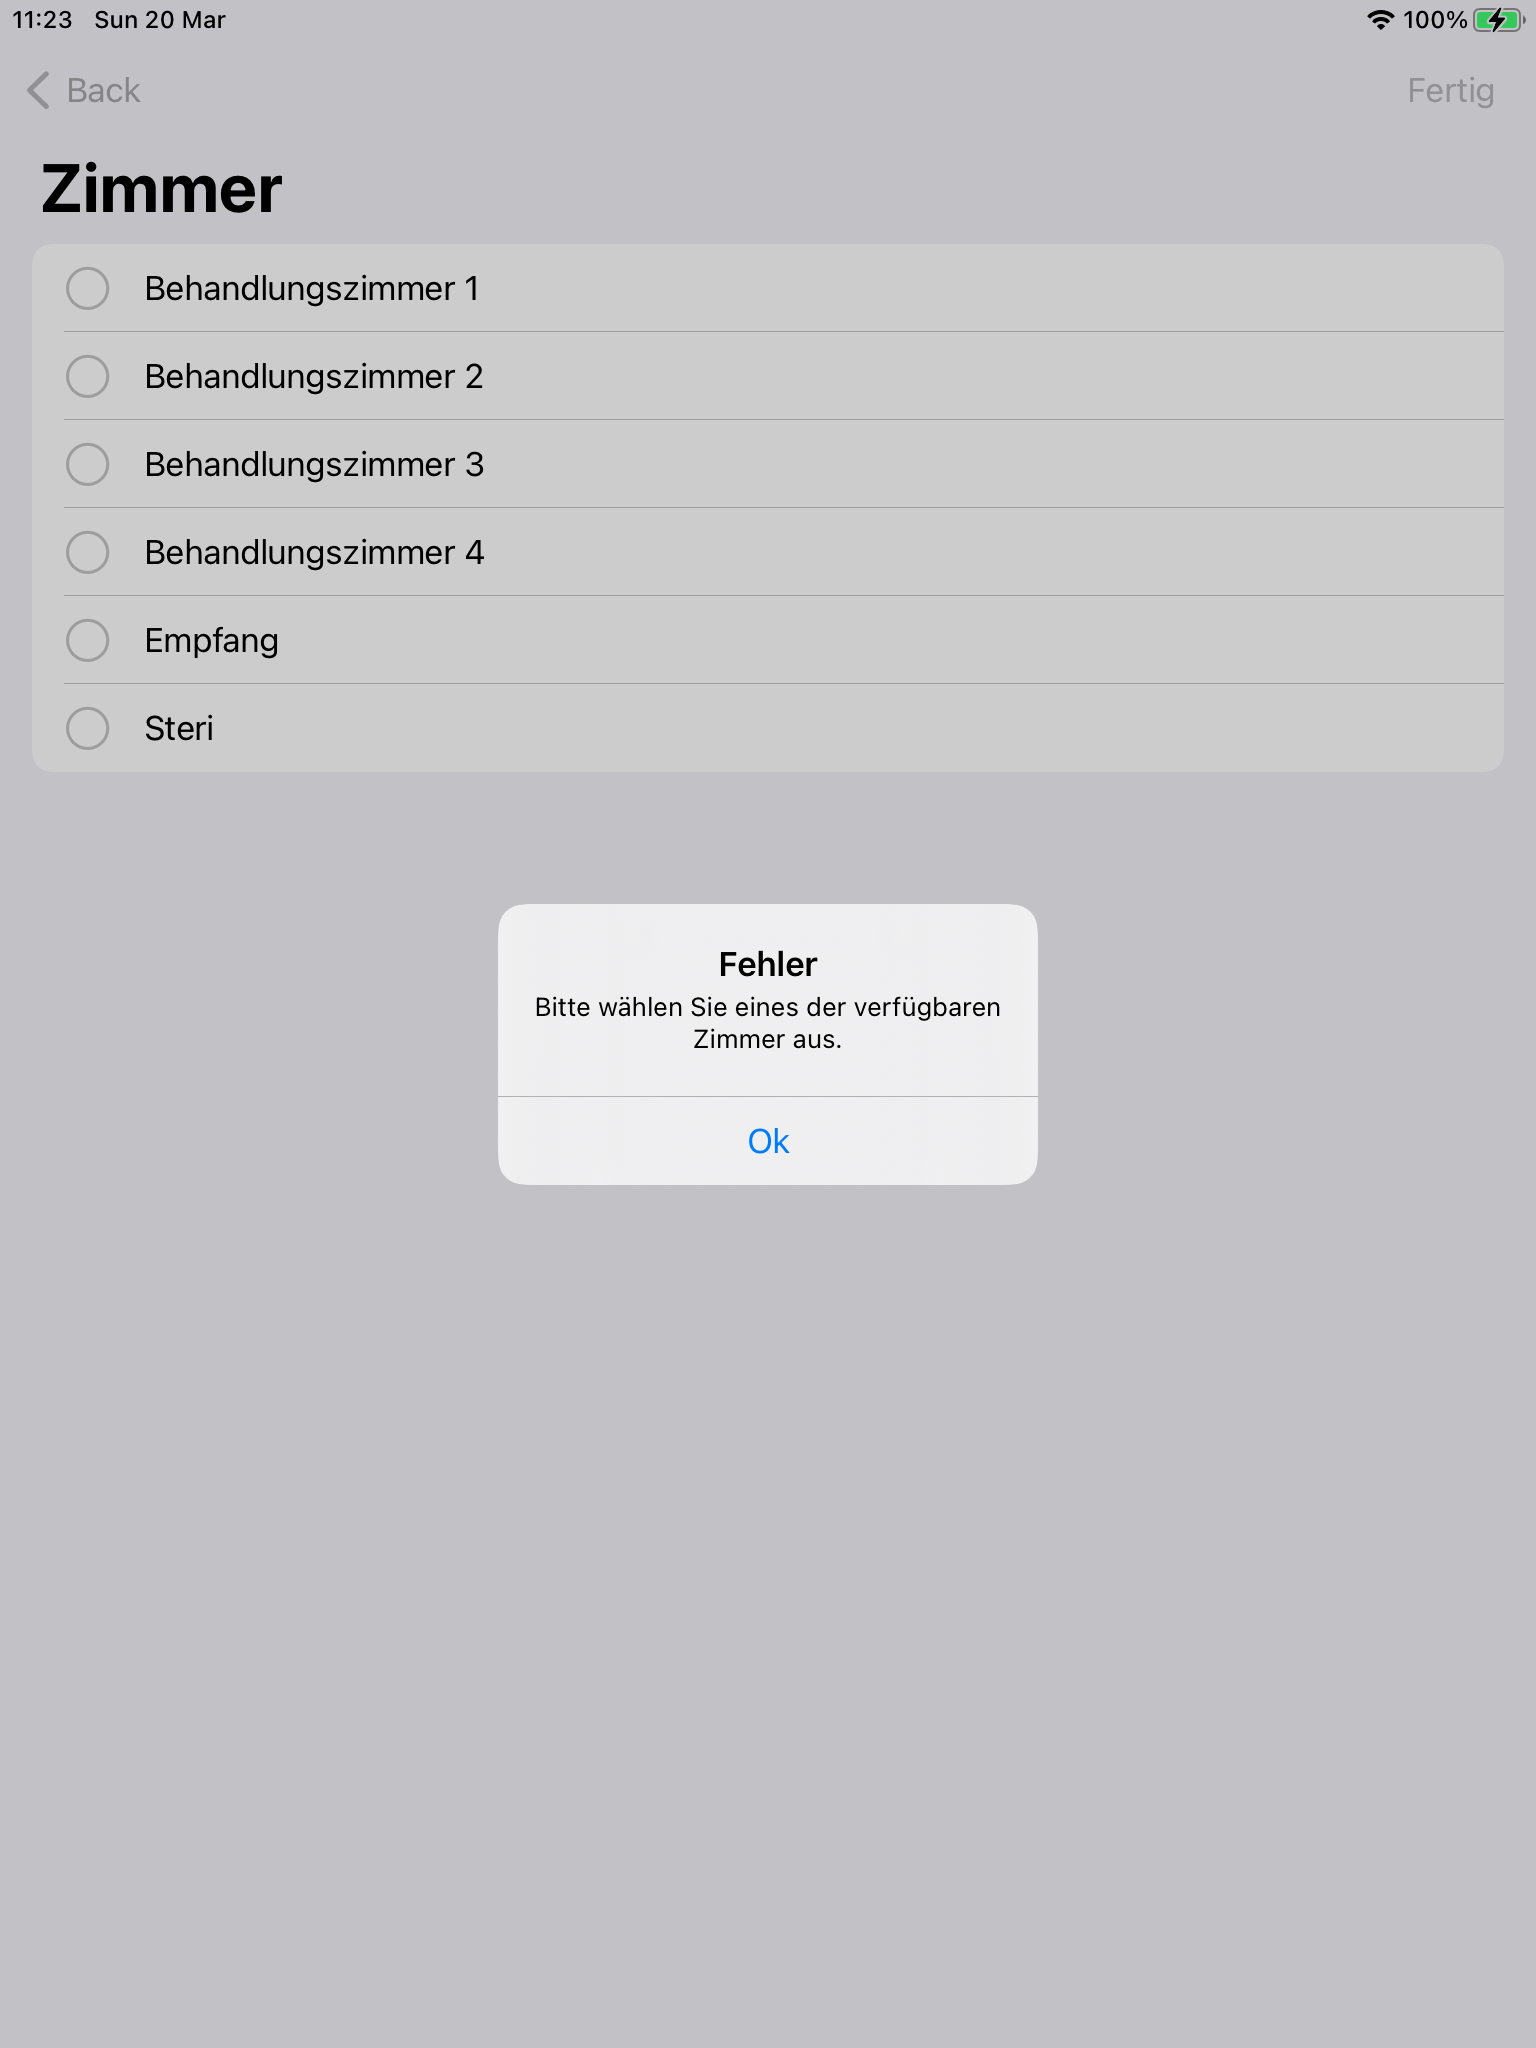
\includegraphics[width=\textwidth]{graphics/screenshots/app/error}}
        \caption{Benachrichtigung wiederholen}
    \end{minipage}
    \label{fig:MobileClient-Screens4}
\end{figure}

Fehler in der Applikation werden dem Benutzer in einem einfachen Dialogfenster angezeigt.
Abbildung 8.x zeigt eine Fehlermeldung, die bei der Auswahl der Zimmerkonfiguration auftreten kann.
Wenn die Wahl der Konfiguration bestätigt wird, ohne dass eine Konfiguration ausgewählt wurde, wird eine entsprechende Fehlermeldung angezeigt.


\clearpage



\subsection{Tests}

\subsubsection{Benutzertests}

Am 11.01.2022 wurden zusammen mit dem Auftraggeber Benutzertests durchgeführt.
Die iOS Applikation wurde auf zwei Physische iPads installiert.
Eine dritte Instanz der Applikation wurde auf einem Simulator gestartet.
Während den Benutzertests wurde folgendes getestet:

\begin{enumerate}
    \item Anmeldung und Konfigurationsauswahl funktioniert wie im Vorgängerprojekt.
    \item Benachrichtigungen können zwischen Mobile Clients versendet werden.
    \item Empfangene Benachrichtigungen werden dem Benutzer vorgelesen.
    \item Sprachverbindungen können über Buttons hergestellt werden.
    \item Sprachverbindungen werden automatisch angenommen.
    \item Über Sprachverbindungen können in Echtzeit Unterhaltungen geführt werden.
    \item Sprachverbindungen können wieder getrennt werden.
\end{enumerate}

Der Kunde hat während den Tests folgende Verbesserungswünsche eingebracht:

\begin{enumerate}
    \item Das Quittieren von Einträgen in der Inbox soll diese direkt löschen.
    \item Das Quittieren von Einträgen in der Inbox soll durch eine Wischgeste möglich sein.
    \item Die Töne für Benachrichtigungen und eingehende Anrufe von den Tönen anderer Apps unteschieden werden können.
    \item Die Töne für Benachrichtigungen und eingehende Anrufe sollen konfigurierbar sein.
    \item Icon und Name der App sollen angepasst werden.
    \item Bei eingehenden Sprachverbindungen soll ein Benachrichtigungston erklingen.
    \item Status von Verbindungsteilnehmern soll als Icon dargestellt werden.
\end{enumerate}

Dieses Feedback konnte grösstenteils umgesetzt werden.
Elemente können per Wischgeste quittiert werden und werden dabei direkt aus der Inbox gelöscht.
Icon und Name der App wurden angepasst.

Bei eingehenden Sprachverbindungen ertönt ein Benachrichtigungston bevor die Verbindung geöffnet wird.
Nachdem die Verbindung geöffnet wird, wird der Status aller Teilnehmenden mit einem einfachen Icon dargestellt.
Es werden unterschiedliche Töne für Benachrichtigungen, Erinnerungen an unquittierte Nachrichten und den Eingang von Sprachverbindungen verwendet.
Dabei werden keine Systemtöne von iOS verwendet.
Dadurch können Praxismitarbeitende die Bedeutung eines Tons aus der Praxisruf-App eindeutig erkennen.
Damit sind die Anforderungen aus Punkten 1.\ bis 3.\ sowie 5.\ bis 7.\ erfüllt.

Der Punkt 4.\ konnte aus Zeitgründen nicht umgesetzt werden.
Alle Töne sind allerdings fest definiert und können nicht durch den Benutzer konfiguriert werden.
Eine Änderung der Töne ist nur über Änderungen am Quellcode möglich.

\clearpage

\subsubsection{Funktionstests}

Im Rahmen des Projektes Peer-To-Peer Kommunikation für Sprachübertragung in einem Praxisrufsystem wurde ein finaler Testplan definiert.
Diese Tests wurden zum Abschluss des Projektes durchgeführt, um die Funktionalität des Systems abschliessend zu testen.
Die Szenarien S01 bis S18 wurden dabei aus dem Vorgängerprojekt ''IP5 Cloudbasiertes Praxisrufsystem'' übernommen.
Dadurch kann sichergestellt werden, dass alle Funktionen aus dem Vorgängerprojekt korrekt migriert wurden.
Die Testszenarien S19 bis S40 behandeln die Funktionen Sprachsynthese und Gegensprechanlage.
Die detaillierte Definition mit Ausgangslage, Testschritten und erwartetem Resultat der Testszenarien sind im Anhang C aufgeführt.

Folgendes Protokoll zeigt den Stand der letzten Ausführung der Tests am 21.03.2022:

\begin{table}[h]
    \centering
    \begin{tabular}{|l|p{11cm}|c|c|}
        \hline
        \textbf{Szenario} & \textbf{Beschreibung} & \textbf{Resultat} \\
        \hline
        S01         & Benachrichtigung versenden - Empfänger konfiguriert   & +\\
        \hline
        S02         & Benachrichtigung versenden - Kein Empfänger konfiguriert & +\\
        \hline
        S03         & Benachrichtigung empfangen.  & +\\
        \hline
        S04         & Fehler beim Versenden anzeigen.  & +\\
        \hline
        S05         & Wiederholen im Fehlerfall bestätigen.  & +\\
        \hline
        S06         & Wiederholen im Fehlerfall abbrechen.  & +\\
        \hline
        S07         & Audiosignal bei Benachrichtigung.   & +\\
        \hline
        S08         & Push Benachrichtigung im Hintergrund.  & +\\
        \hline
        S09         & Erinnerungston für nicht quittierte Benachrichtigungen.   & +\\
        \hline
        S10         & Start Mobile Client - Nicht angemeldet   & +\\
        \hline
        S11         & Start Mobile Client  - Angemeldet & +\\
        \hline
        S12         & Anmelden mit korrekten Daten.   & +\\
        \hline
        S13         & Anmeldung mit ungültigen Daten.   & +\\
        \hline
        S14         & Konfiguration Wählen   & +\\
        \hline
        S15         & Abmelden   & +\\
        \hline
        S16         & Admin UI - Anmeldung mit korrekten Daten   & +\\
        \hline
        S17         & Admin UI - Anmeldung mit ungültigen Daten   & +\\
        \hline
        S18         & Admin UI - Konfiguration Verwalten   & +\\
        \hline
        S19         & Benachrichtigung vorlesen - Sprachsynthese aktiviert und Benachrichtigung relevant & +\\
        \hline
        S20         & Benachrichtigung nicht vorlesen - Sprachsynthese aktiviert und Benachrichtigung nicht relevant & +\\
        \hline
        S21         & Lokale Einstellung - Sprachsynthese deaktiviert und Benachrichtigung relevant  & +\\
        \hline
        S22         & Lokale Einstellung - Sprachsynthese deaktiviert und Benachrichtigung nicht relevant  & +\\
        \hline
        S23         & Benachrichtigung verwalten - Relevanz Sprachsynthese kann im Admin UI aktiviert / deaktiviert werden  & +\\
        \hline
        S24         & Benachrichtigung empfangen - Änderung an Inhalt einer Benachrichtigung in Admin UI wird sofort angewendet   & +\\
        \hline
        S25         & Gegensprechanlage Buttons nach Anmeldung anzeigen & +\\
        \hline
        S26         & Verbindungsaufbau - Gegenüber ist Verfügbar & +\\
        \hline
        S27         & Verbindungsaufbau - Gegenüber ist nicht Verfügbar & +\\
        \hline
        S28         & Verbindungsaufbau - Gegenüber hat Gegensprechanlage deaktiviert & +\\
        \hline
        S29         & Verbindungsaufbau - Benachrichtigungston & +\\
        \hline
    \end{tabular}\label{tab:funktion_testplan_1}
\end{table}

\clearpage

\begin{table}[h]
    \centering
    \begin{tabular}{|l|p{11cm}|c|c|}
        \hline
        \textbf{Szenario} & \textbf{Beschreibung} & \textbf{Resultat} \\
        \hline
        S30         & Verbindungsaufbau - Automatische Annahme & +\\
        \hline
        S31         & Unterhaltung 1:1 - Unterhaltung in Echtzeit möglich & +\\
        \hline
        S32         & Unterhaltung 1:n - Unterhaltung in Echtzeit möglich & +\\
        \hline
        S33         & Verbindungsaufbau 1:n & +\\
        \hline
        S34         & Inbox - Vergangene Sprachverbindungen & +\\
        \hline
        S35         & Inbox - Verpasste Sprachverbindungen & +\\
        \hline
        S36         & Inbox - Abgelehnte Unterhaltungen & +\\
        \hline
        S37         & Verbindung trennen durch Empfänger & +\\
        \hline
        S38         & Verbindung trennen durch Initiator & +\\
        \hline
        S39         & Austreten aus Gruppenunterhaltung & +\\
        \hline
        S40         & Konfiguration über Admin UI & +\\
        \hline
    \end{tabular}\label{tab:funktion_testplan_2}
\end{table}

Alle Testszenarien konnten mit einem positiven Resultat abgeschlossen werden.
Das System erfüllt damit die Anforderungen, die im Rahmen dieses Projektes an ein Praxisrufsystem gestellt werden.
Das umgesetzte System weist aber durchaus noch Potential zur Weiterentwicklung auf.

Im Bereich Gegensprechanlage, besteht Optimierungspotential für das Entgegennehmen von Anrufen.
Das Empfangen von Anrufen ist aktuell nur möglich, wenn die Praxisruf-App aktiv ist.
Ist die App nicht aktiv, werden Empfänger über Benachrichtigungen auf verpasste Anrufe hingewiesen.
Das Antippen dieser Benachrichtigungen öffnet die Praxisruf-App.
Es wird dabei aber kein Anruf entgegengenommen.
Für die Weiterentwicklung des Systems wäre es ideal, wenn das Öffnen einer Benachrichtigung für verpasste Anrufe einen direkten Rückruf ermöglicht.

Die Benutzeroberflächen des Mobile Clients erlaubt eine effiziente Bedienung des Systems.
Design und User Experience der Applikationen könnten aber weiter verbessert werden.
Für die Weiterentwicklung der App sollte die Applikation zusammen mit Praxismitarbeitenden getestet werden.
So können diese Rückmeldung zur Bedienung der App geben.
Basierend darauf kann die App für Bedürfnisse der Anwendenen optimiert werden.

Weiter hat das System noch Lücken die auf das Vorgängerprojekt zurückzuführen sind.
Diese Verbesserungen sind ausserhalb des Umfangs dieses Projektes gefallen, sollten für die Weiterentwicklung von Praxisruf aber berücksichtigt werden.
Insbesondere das Quittieren von Benachrichtigungen und die Konfigurationsverwaltung könnten verbessert werden.

Das Quittieren von Benachrichtigungen ist mit dem aktuellen System nur lokal auf dem Empfängergerät möglich.
Für die Weiterentwicklung des Systems wäre es wünschenswert, dass ein Sender über die Quittierung von Benachrichtigungen informiert wird.
So kann er sicher sein, dass die Benachrichtigung empfangen und gelesen wurde.

Das Admin UI ermöglicht heute die Konfiguration des Systems.
Die Konfiguration des Systems könnte aber weiter optimiert werden.
Heute ist es nicht möglich, die Konfiguration für ein Zimmer mehrfach zu verwenden.
Dies bedeutet, dass Praxisadministrierende manche Konfigurationen mehrfach erfassen müssen.
Weiter verwendet die Benutzeroberfläche des Admin UI ausschliesslich technische Begriffe für die Konfigurationseinheiten.
Für die Weiterentwicklung des Systems sollten sprechende Begriffe in der Benutzeroberfläche verwendet werden.
Die Konfiguration des Systems sollte vereinfacht werden, so dass keine doppelten Konfigurationen vorgenommen werden müssen.

Das System bringt noch diverse Lücken aus dem Vorgängerprojekt mit sich und hat Potential sich in den Bereichen Benutzerfreundlichkeit und Stabilität zu verbessern.
Trotz dieser Lücken werden die funktionalen Anforderungen, die im Rahmen dieses Projektes an Praxisruf gestellt wurden, erfüllt.
Die Funktionstests sind dadurch mit einem positiven Resultat abgeschlossen.
Das System kann in der aktuellen Form eingesetzt werden.
Für den langfristigen Erfolg des Systems, sollten die bekannten Lücken allerdings bei der Weiterentwicklung adressiert werden.

\subsubsection{Performancetests}

Neben Szenarien für Funktionstests, wurden einfache Tests zur Messung der Performance des Systems definiert.
Dazu wurden die Performancekriterien P01 bis P08 definiert.
Folgendes Protokoll zeigt den Stand der letzten Ausführung der Tests am 21.03.2022.

\begin{table}[h]
    \centering
    \begin{tabular}{|l|p{11cm}|c|c|}
        \hline
        \textbf{Kriterium} & \textbf{Beschreibung} & \textbf{Resultat} \\
        \hline
        P01         & Zeit bis Benachrichtigung ankommt im Schnitt $<$ 5s & +\\
        \hline
        P02         & Vorlesen von Benachrichtigung $<$ 5s nach Benachrichtigungston (ohne Cache) & +\\
        \hline
        P03         & Vorlesen von Benachrichtigung $<$ 5s nach Benachrichtigungston (mit Cache) & +\\
        \hline
        P04         & Verbindungsaufbau Sprachverbindung $<$ 5s  & +\\
        \hline
        P05         & Verzögerung bei Sprachverbindung klein um kurze Gespräche zu führen & +\\
        \hline
        P06         & Ressourcenverbrauch der Applikation bleibt über Zeit konstant & +\\
        \hline
        P07         & Übertragungsqualität von Sprachverbindungen ist ausreichend für normale Unterhaltungen & +\textbackslash- \\
        \hline
        P08         & Verbindung zur Signaling Instanz bleibt geöffnet und wird bei Fehlern automatisch wiederhergestellt. & +\textbackslash- \\
        \hline
    \end{tabular}\label{tab:testplan_performance}
\end{table}

Die Performancekriterien P01 bis P06 sind vollständig erfüllt.
Die Kriterien P07 und P08 sind mit Einschränkungen erfüllt und zeigen, dass das die Performance des Systems weiter verbessert werden könnte.

Das Kriterium P07 wird mit Einschränkungen erfüllt.
Die Qualität der Sprachverbindungen ist ausreichend für eine Gegensprechanlage.
Es ist problemlos möglich Unterhaltungen über die aufgebaute Sprachverbindung zu führen.
Probleme können entstehen, wenn eine Verbindung zwischen Endgeräten aufgebaut wird, welche nahe beieinander installiert sind.
In diesem Fall können Rückkoppelungen entstehen, welche zu einem Echo und schrillen Pfeifton führen kann.
Dieses Problem ist durch eine entsprechende Ausrichtung der Geräte vermeidbar.
Es schränkt aber ein, wie die Endgeräte des Systems in einer Praxis installiert werden können.

Das Kriterium P08 ist grundsätzlich erfüllt.
Wenn die Verbindung zur Signaling Instanz verloren geht, wird eine Fehlermeldung angezeigt.
Die Verbindung wird danach sobald möglich automatisch wiederhergestellt.
Dies wurde mehrmals über einen Zeitraum von 12h getestet und hat zuverlässig funktioniert.
Dabei ist es in Einzelfällen dazu gekommen, dass die Fehlermeldung angezeigt wird, obwohl es keinen ersichtlichen Grund gibt, dass die Verbindung getrennt wurde.
Nach Bestätigung des Dialogs, konnte die Verbindung in jedem Fall wiederhergestellt werden.
Versuche dieses Verhalten gezielt zu reproduzieren waren nicht erfolgreich.
Da die Verbindung in jedem Fall wiederhergestellt werden konnte, wird das Kriterium P08 als erfüllt betrachtet.
Für die Weiterentwicklung des Systems, sollte die Verbindungsverwaltung in einem produktionsnahen Umfeld getestet werden.
Dabei kann die Performance des Systems beobachtet werden und wenn nötig Korrekturen an der Verwaltung vorgenommen werden.

Letztlich haben Installationstests des Releases für die Praxisruf-App gezeigt, dass die initiale Installation des Systems aufwändig sein kann.
In einzelnen Testdurchläufen konnten direkt nach der Installation keine Sprachverbindungen aufgebaut werden.
Dieses Problem konnte darauf zurückgeführt werden, dass die Berechtigungen, welche für Netzwerkverbindungen benötigt werden, nicht korrekt angefordert wurden.
In der Installationsanleitung (Anhang D) wird beschrieben, wie dieses Problem bei der Installation gelöst werden kann.
Für die Weiterentwicklung des Systems wäre es wünschenswert, dass alle Berechtigungen automatisch und zwingend beim Start der Applikation angefordert werden.

Die Performancetests konnten mit einem positiven Resultat abgeschlossen werden.
Das System kann trotz der bekannten Lücken effizient bedient und als Praxisrufsystem verwendet werden.
Die bekannten Lücken sollten aber mit Weiterentwicklung von Praxisruf geschlossen werden.

\clearpage

\subsection{Fazit}

In diesem Kapitel werden die zentralen Herausforderungen während der Projektarbeit und die Schlussfolgerungen die daraus gezogen werden können beschrieben.

Eine grosse Herausforderung in diesem Projekt, war die Konzipierung und Umsetzung des nativen Mobile CLients.
Insbesondere die effiziente Anbindung an die Umsysteme Cloudservice und Messagingservice sowie die Integration von Sprachverbindungen mit WebRTC stellten eine Herausforderung dar.
Die iOS Standardbibliothek sowie die iOS SDKs für WebRTC und Firebase Cloud Messaging und bieten alle Komponenten, welche für diese Integration notwendig sind.
Die Herausforderung bestand darin, diese Komponenten effizient zu verwenden und Strukturen aufzubauen, welche die Integration in eine SwiftUI Applikation ermöglichen.
Das Erarbeiten dieser Konzepte hat mehr Zeit in Anspruch genommen als erwartet und hat einen grösseren Teil des Konzepts in Anspruch genommen als erwartet.
Dieser Mehraufwand hat sich schlussendlich aber bezahlt gemacht.
Die Anbindungen an Umsysteme und Peer To Peer Verbindungen konnte in eigenen Komponenten gekapselt, welche effizient in SwiftUI eingebunden werden können.\footnote{Siehe Kapitel 5}
Im Unterschied zur Entwicklung des Shared Platform Mobile Clients im Vorgängerprojekt, konnte der Aufwand hier mehrheitlich auf konzeptioneller Ebene gehalten werden.
Die Anbindung der Schnittstellen und insbesondere die Verwendung von Gerätehardware und Betriebssystemfunktionen wie Pushbenachrichtigungen konnt deutlich einfacher umgesetzt werden.
Es sind keine Probleme bezüglich Kompatibilität oder nicht unterstützten Funktionen aufgekommen.

Ich schliesse daraus, dass sich die native Mobile Entwicklung mit SwiftUI grundsätzlich besser für eine Praxisruf Applikation eignet als die Shared Platform Entwicklung.
Um dies effizient zu machen, ist es allerdings unerlässlich, dass die Konzepte zur Anbindung von Umsystemen und direkten Verbindungen sauber erstellt werden.
Die Verantwortlichkeit interne Komponenten muss klar definiert und der Aufbau effizient implementiert sein.
Ist dies gegeben, kann am ende ein gutes Produkt stehen.

Das Erarbeiten der Konzepte für die Einbindung von WebRTC waren aus weiteren Gründen mühsam.
Wie auch Firebase Cloud Messging (FCM) bietet WebRTC einen nativen iOS SDK.
Im Unterschied zu FCM bietet WebRTC allerdings keine nennenswerte Entwicklerdokumentation.
Dieses Risiko wurde bereits bei der Evaluation der Technologie\footnote{Siehe Kapitel 4} erkannt.
WebRTC wurde trotzdem für dieses Projekt verwendet, da es Providerunabhängigkeit und maximale Flexibilität bei der Integration in das System bietet.
Diese Vorteile konnten beim Projekt wirklich genutzt werden.
Der Signalingservice ist komplett Providerunabhängig und kann bei einem beliebeingen Cloudprovider oder auf einem eigenen Server betrieben werden.
Die Sprachverbindungen die im Mobile Client aufgebaut werden sind direkte Peer To Peer Verbindungen, auch dafür wird keine zusätzliche Instanz benötigt.
Die mangelhafte Dokumentation hat die Umsetzung dieser Lösung allerdings deutlich erschwert.
Es finden sich viele öffentlich zugängliche Referenzimplementierungen und einfache Anleitungen zur Integration von WebRTC in Applikationen.
Diese sind in aller Regel aber sehr simpel gehalten.
Sie beinhalten keine Mechanismen zum Verbindungsmanagement und keine saubere Integration in die Benutzeroberfläche.
Die Komponenten aus dem WebRTC SDK werden kommentarlos verwendet.
Dieses Problem wird ein Stück weit dadurch relativiert, dass WebRTC eine Open Source Technologie ist die von allen grossen Browsern unterstützt wird.
Die Konzepte welche für den Verbindungsaufbau mit WebRTC verwendet werden, sind deshalb an vielen Orten beschrieben.
Die Komponenten und Konzepte in WebRTC sind dabei Platformunabhängig dieselben.
Dementsprechend konnten diese Resourcen verwendet werden, um das System zu versehen und auf die eigenen Anforderungen zugeschnitten umzusetzen.
Schlussendlich konnte hier eine Lösung umgesetzt werden, die alle Anforderungen einer Gegensprechanalge im Praxisrufsysteme rfüllt.

Aus den Erfahrungen mit WebRTC im iOS Umfeld schliesse ich darauf, das WebRTC durchaus geeignet ist um ein Praxisrufsystem umzusetzen.
Die Unabhängigkeit von Providern bringt grosse Flexibilität und Unabhängigkeit mit sich.
Gleichzeitig, muss aber betrachtet werden, dass WebRTC eine Open Source Technologie von Google ist.
Es gibt keine Garantie wie lange WebRTC weiterentwickelt wird oder dass es mit zukünftigen iOS Versionen kompatibel bleibt.
WebRTC selbst ist aber ein offener Standard und Google liefert lediglich die Implementation.
Da es heute in allen grossen Browsern unterstützt ist, ist es wahrscheinlich dass es in jedem Fall von jemandem weiterentwickelt wird.
Um sicherzustellen, dass ein Praxisrufsystem das WebRTC verwendet langfristig erfolgreich bleibt, muss eine entsprechende Ausstiegsstrategie definiert werden.
Dies beinhaltet zeitnahe evaluation neuer iOS Releases um die Kompatibilität mit WebRTC sicherzustellen.
Es beinhaltet weiter ein Konzept, wie WebRTC durch eine andere Technologie ersetzt werden kann.
Im Rahmen dieser Projektarbeit konnte kein solches Konzept erstellt werden.
Es wird empfohlen für die Weiterentwicklung von Praxisruf ein solches Konzept zu erstellen.


Covid war auch eine Challange.
Im Methoden Teil wurde angedacht, dass scrum mässig zusammengesessen und getestet wird.
Das hat aus zwei gründen nicht ganz wie erwartet funktioniert.
Einerseits, ist der Konzept teil zu lang.
Nicht länger als angedacht, aber halt doch lang.
Meetings mussten grösstenteils remote statfinden.
Das hat Demonstartionen und Absprachen deutlich erschwert.
Anforderungen wurden am Anfang gemacht, das ist auch gut so.
Persönlichere Meetings hätten aber vlt direkteres Feedback ermöglicht, so dass direkter auf Bedürfnisse hätte eingegangen werden können.
Letztlich bin ich selbst am Covid erkrankt.
Genau in der Zeit in der ich vorgenommen hatte, Zeit für das Projekt zu investieren.
Das hat zu Verzögerungen geführt.
Insgesamt trotzdem erreicht.
Aber es könnte besser sein.
Anforderungen waren als Minimum gedacht, mit raum für mehr.

Fazit: Puffer sind nötig.
Es wurde Zeit für Polishing eingeplant aber nicht genug.
Künftig: Puffer explizit als Puffer einbauen und nicht als Zeit in der man erwartet noch mehr machen zu können.
Mehr Zeit für Testing
Mehr Zeit für Polishing

Insgesamt bin ich mit dem Resultat dieser Arbeit sehr zufrieden.
Ich bin sehr zufrieden mit der Systemarchitektur.
Überzeugt, dass diese verwendet werden kann um ein gutes, kommerzielles Produkt zu erstellen.
Ich bin weiter zufrieden mit dem Aufbau des Mobile Clients.
Besonders da es mein erster ist.
Besonders Anbindung umsysteme und integration in UI.
Gleichzeitig hätte ich mir gwünscht weiter zu kommen.
Es wurden gerade die minimalen Anforderungen unmgesetzt, die am Anfang definiert wurden.
Eigentlich hätte ich mehr gewollt.

Unterm Strich: Ein guter Prototyp der als Basis für eine kommerzialisierung eines Cloudbasierten Praxisrufsystems dienen kann.


\clearpage

    \section{Schluss}

Im Rahmen dieser Projektarbeit wurde Sprachübertragung und Sprachsynthese in ein cloudbasiertes Praxisrufsystem integriert.
Die umgesetzte Lösung basiert auf dem Praxisrufsystem das im Rahmen des Projektes ''Cloudbasiertes Praxisrufsystem'' umgesetzt wurde.\cite{ip5}
Das erweiterte System besteht aus einer Mobilen Applikation, einem Cloudservice und einer Web-Applikation.
Die Mobile Applikation wurde neu als native Applikation für iOS entwickelt.
Sie ersetzt die Shared Platform Applikation, welche im Rahmen des Vorgängerprojektes entwickelt wurde.
Dabei wurden sämtliche Funktionen und Anbindungen an Umsysteme auch in der neuen Applikation implementiert.
Mit diesem Projekt neu konzipiert und umgesetzt wurden die Sprachsynthese für empfangene Benachrichtigung mit ''AWS Polly '' sowie die Integration einer Gegensprechanlage über Peer To Peer Verbindungen.

Das umgesetzte Praxisrufsystem kann zum Austausch von Informationen in einem Praxisumfeld verwendet werden.
Als Endgeräte dienen dabei iOS Tablets.
Über die Mobile Applikation des Systems ist es möglich Sprachverbindungen zu einem oder mehreren anderen Clients aufzubauen.
Eingehende Sprachverbindungen werden automatisch angenommen.
Das System unterstützt weiter das Versenden und Empfangen von Benachrichtigungen.
Dies wird einerseits verwendet, um nicht erreichbare Empfänger über verpasste Sprachverbindungen zu informieren.
Weiter bietet die Applikation Praxismitarbeitenden die Möglichkeit vorkonfigurierte Benachrichtigungen an andere Clients zu versenden.
Der Inhalt von Benachrichtigungen kann dabei beim Empfang automatisch vorgelesen werden.
Sowohl empfangene Benachrichtigungen als auch verpasste und vergangene Anrufe, werden gesammelt und in einer Inbox angezeigt.
Empfangene Benachrichtigungen und verpasste Anrufe müssen von Praxismitarbeitenden quittiert werden.
Sind unquittierte Elemente in der Inbox, ertönt in regelmässigen Abständen ein Erinnerungston.

Das umgesetzte System deckt die wesentlichen Anforderungen eines cloudbasierten Praxisrufsystems ab.
Für eine kommerzielle Nutzung des Systems sind aber zusätzliche Erweiterungen notwendig.
Praxisruf unterstützt in der aktuellen Version die Authentifzierung mittels Json Web Tokens.
Ausstellung der Tokens wird dabei allerdings durch Praxisruf selbst gemacht.
Es wird empfohlen vor der kommerziellen Nutzung einen externen Identity Provider anzubinden und Authentifizierung/Authorisierung nach OpenID Connect umzusetzen.
Weiter ist Praxisruf heute nur beschränkt mandantenfähig.
Praxismitarbeitende haben nur Zugriff auf Konfigurationen, welche dem verwendeten Benutzer zugewiesen sind.
Praxisadministratoren können allerdings immer alle bekannten Konfigurationen über das Admin UI verwalten.
Weiter wird bei der Auswertung der Konfiguration für das Zustellen von Benachrichtigungen und beim der Signalvermittlung für Sprachverbindungen keine Zuordnung an Benutzer oder Mandat geprüft.
Um Praxisruf produktiv bei mehreren Kunden einzusetzen, muss es Mandantenfähigkeit implementiert werden.
Letztlich sind heute einfache Mechanismen für das Wiederholen von Benachrichtigungen und Wiederaufbau von verlorenen Verbindungen implementiert.
Für den produktiven Betrieb können und müssen diese allerdings noch erweitert werden.
Insbesondere der Wiederaufbau von bestehenden Sprachverbindungen bei Verbindungsverlust ist für eine kommerzielle Nutzung unerlässlich.

Die grösste Gefahr für die produktive Nutzung von Praxisruf ist allerdings, das es bis heute nie in grösserem Umfang produktiv eingesetzt wurde.
In der aktuellen Form sollte Praxisruf nicht im grossen Stil produktiv eingesetzt werden.
Es bietet allerdings alle Funktionen, die ein Praxisrufsystem benötigt.
Dementsprechend ist es möglich, das System in einem Pilotbetrieb einzusetzten.
So kann Testfeedback von Benutzern eingeholt werden und es können Performance Metriken gesammelt werden.
Diese können weitere Einblicke darauf geben, welche Teile des Cloudservices separat als skalierbare Microservices deployed werden sollen.
Wird Praxisruf mit den Erkentnissen aus einem Pilotbetrieb ergänzt und die Funktionen Mandantenfähigkeit und OpenId Connect implementiert, kann es kommerziell und produktiv genutzt werden.

Insgesamt bin ich mit den Konzepten und Ergebnissen, die aus dieser Arbeit hervorgegangen sind zufrieden.
Ich bin überzeugt, dass die erarbeiteten Konzepte und das umgesetzte System eine solide Grundlage für ein kommerziell erfolgreiches cloudbasiertes Praxisrufsystem bilden.

%Insgesamt bin ich mit dem Resultat dieser Arbeit zufrieden.
%Die erarbeitete Architektur bietet eine solide Basis für ein cloudbasiertes Praxisrufsystem.
%Das umgesetzte System bietet einen voll funktionsfähigen Prototypen.
%Dieser kann als Basis für die Entwicklung eines kommerziell erfolgreichen Systems verwendet werden.







\clearpage



%%---APPENDIX----------------------------------------------------------------------------
    \renewcommand\refname{Literaturverzeichnis}
\addcontentsline{toc}{section}{Literaturverzeichnis}
\printbibliography
\cleardoublepage
\listoffigures

\appendix
\clearpage
\section{Aufgabenstellung}\label{sec:aufgabenstellung}
\begin{figure}[h]
    \centering
    \begin{minipage}[b]{0.8\textwidth}
        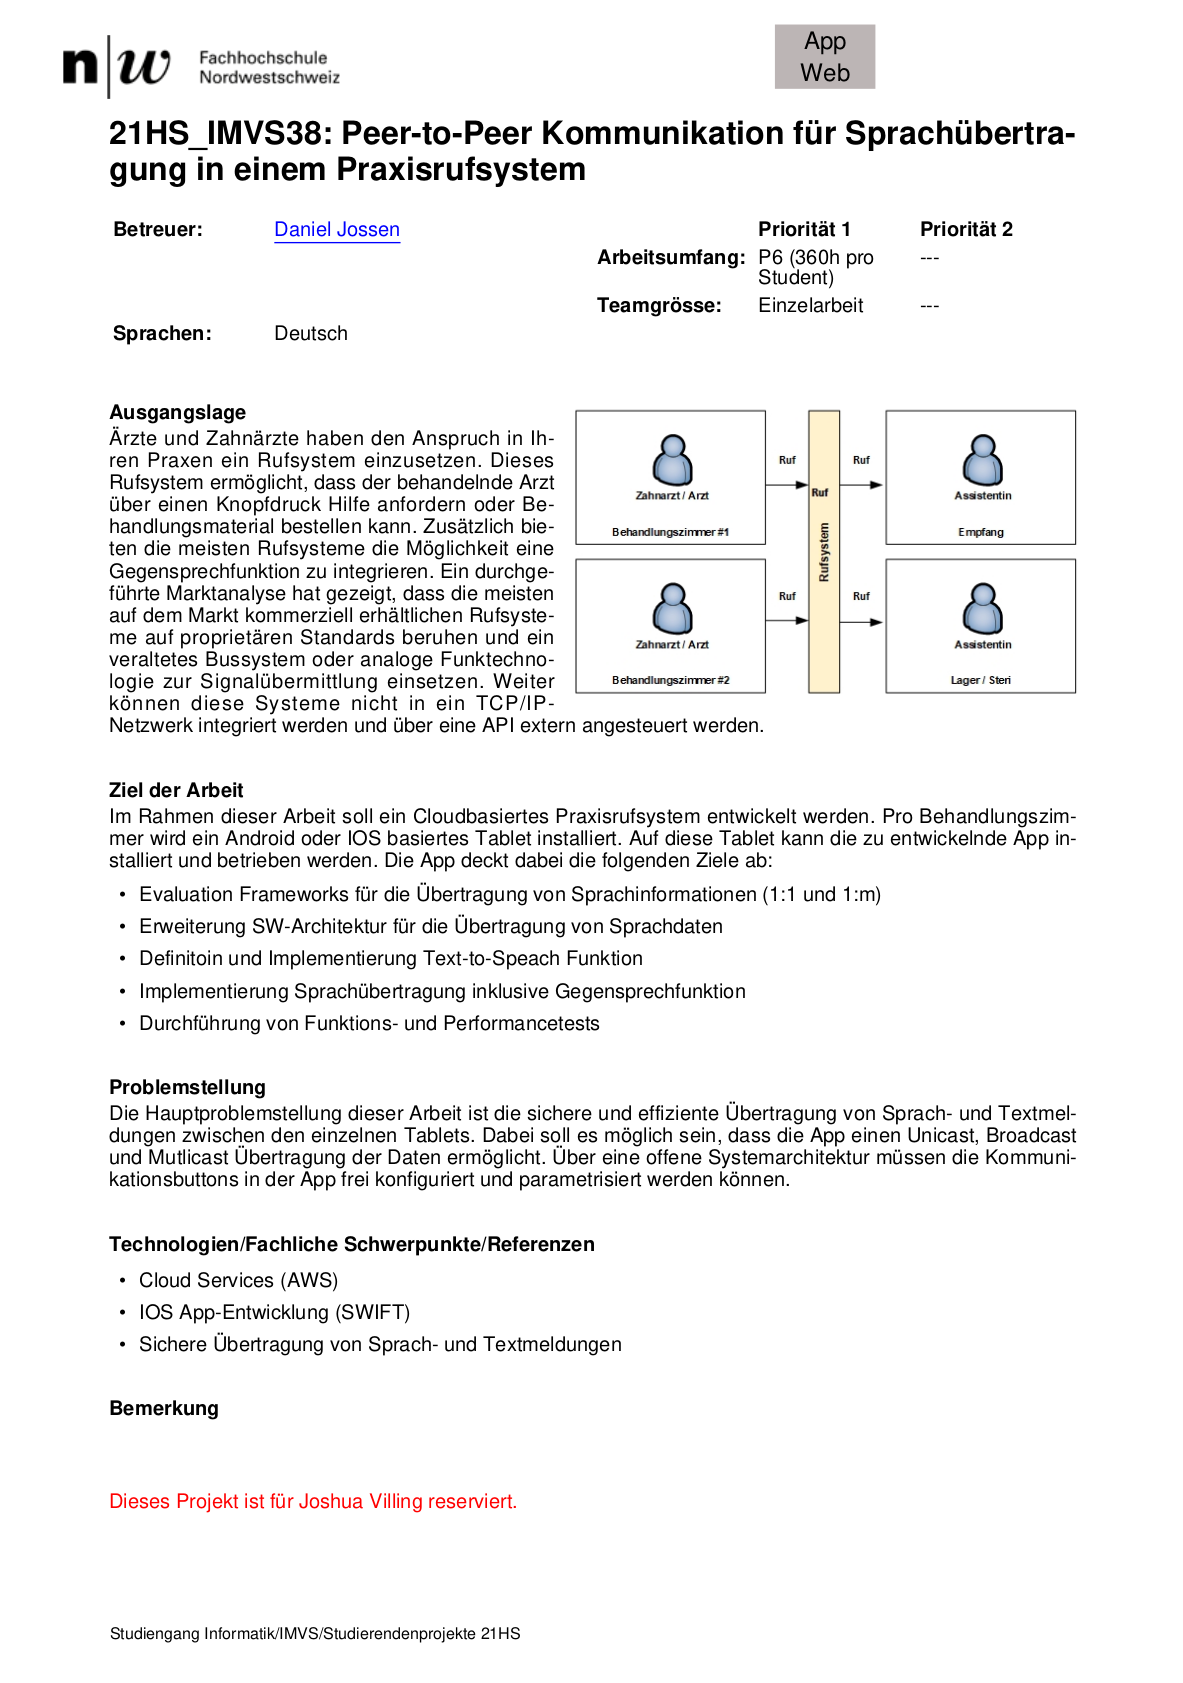
\includegraphics[width=\textwidth]{graphics/aufgabenstellung}
        \caption{Aufgabenstellung}
    \end{minipage}\label{fig:aufgabenstellung}
\end{figure}

\clearpage

\section{Quellcode}\label{sec:quellcode}

Sämtlicher Quellcode der im Rahmen des Projektes entsteht, wurde mit Git verwaltet. Der Quellcode ist für Berechtigte unter github.com einsehbar\footnote{\url{https://github.com/users/jsvilling/projects/3}}.
Berechtigungen können bei Joshua Villing angefordert werden.

\clearpage

\section{Ehrlichkeitserklärung}

«Hiermit erkläre ich, die vorliegende Projektarbeit IP6 - Cloudbasiertes Praxisrufsystem selbständig und nur unter Benutzung der angegebenen Quellen verfasst zu haben.
Die wörtlich oder inhaltlich aus den aufgeführten Quellen entnommenen Stellen sind in der Arbeit als Zitat bzw. Paraphrase kenntlich gemacht.
Diese Projektarbeit ist noch nicht veröffentlicht worden.
Sie ist somit weder anderen Interessierten zugänglich gemacht noch einer anderen Prüfungsbehörde vorgelegt worden.»

\begin{tabbing}
    \\
    \\
    \\
    Left \= Middle \=  \= Right \kill
    Name \> \> \>    Joshua Villing\\
    Ort \> \> \>    Aarau \\
    Datum \> \> \>    01.03.2022\\
    \\
    Unterschrift \> \> \>     ............................\\

\end{tabbing}




\end{document}
